\documentclass[../main.tex]{subfiles}

\begin{document}

\section{Optimal Control of Pitch/Travel without Feedback}\label{kap:Part2OptimalControlWithoutFeedback}

\subsection{Derivation of a continous time state space model}
In this part of the exercise we will disregard elevation, therefore we assume $ e = 0 $ and do include it in the model.

The state-vector, $\bm x$ is defined as:
\begin{equation}\label{eq:lab2_state}
	\bm x = 
	\begin{bmatrix}
		\lambda & r & p & \dot p
	\end{bmatrix}
	^T ,
\end{equation}
where $\lambda$ is travel, $r$ is the travel rate, $p$ is pitch and $\dot{p}$ is pitch rate.

The dynamic equations for the system was given in the problem description \todo{Add ref to page and paper}. These following equations were given:
\begin{subequations} \label{eq:lab2_states_eq}
	\begin{align}
		\dot \lambda &= r \\
		\dot r &= -K_2 p, \quad K_2 = \frac{K_p l_a}{J_t}\\
		\dot p &= \dot p \\
		\ddot p &= -K_1 V_d = K_1 K_{pd} \dot p - K_1 K_{pp} p + K_1 K_{pp} pc, \quad K_1 = \frac{K_f l_h}{J_p}
	\end{align}
\end{subequations}
The state-space form of the system therefore becomes: 
\begin{equation}\label{eq:lab2_cont_ss}
	\underbrace{\begin{bmatrix}
		\dot \lambda \\
		\dot r \\
		\dot p \\
		\ddot p
	\end{bmatrix}}_{\bm{\dot x}} = 
	\underbrace{
	\begin{bmatrix}
		0 & 1 & 0 & 0 \\
		0 & 0 & -K_2 & 0 \\
		0 & 0 & 0 & 1 \\
		0 & 0 & -K_1 K_{pp} &  -K_1 K_{pd}
	\end{bmatrix}
	}_{\bm A_c}
	\begin{bmatrix}
		\lambda \\ r \\ p \\ \dot{p} \\
	\end{bmatrix}
	+
	\underbrace{
		\begin{bmatrix}
			0 \\ 0 \\ 0 \\ K_1 K_{pp}
		\end{bmatrix}
	}_{\bm B_c} \underbrace{p_c}_{u}
\end{equation}

\subsubsection{A deeper dive into the state-space model}
The state-space form of the system models two part of the whole system, namely: 
\begin{enumerate}
	\item The physics of the helicopter.
	\item The proportional-derivative controller for the pitch.
\end{enumerate}
This is shown in \cref{fig:lab2_system} where the red dotted box shows what we model with the state space model. \todo[inline]{Add ref to the figure in the problem description}

\begin{figure}[h]
	\centering
	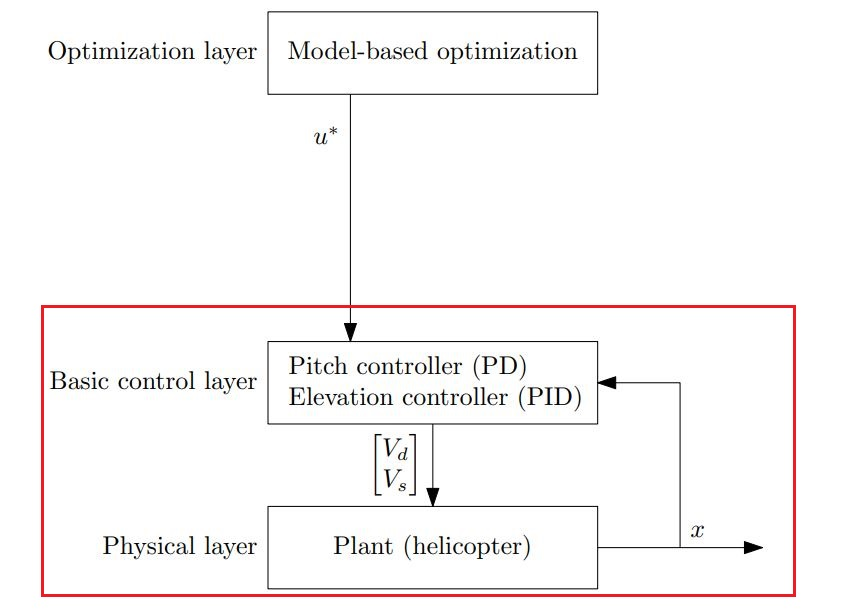
\includegraphics[width=0.8\linewidth]{figures/lab2_system}
	\caption{The red box encapsulate what is modelled in the state space model described by \cref{eq:lab2_cont_ss}.}
	\label{fig:lab2_system}
\end{figure}

This becomes clear studying the equations in \cref{eq:lab2_states_eq}. They describe the helicopters physics for all states except elevation and elevation rate. $ \lambda $ and $ r $ is dependent on the helicopters pitch, $ p $. $ p $ and $ \dot p  $ is however dependent on the voltage difference, $ V_d $. The voltage difference is the output of the PD-controller for controlling the pitch\todo{Should we add acronym list?}. 

To summarize, this means that our state space model describes the helicopter's physics through the dynamic equations for $ \lambda $, $ r $, $ p $ and $ \dot p $, while the equation of $ V_d $ describes the PD-controller used to control the pitch angle. In total our state-space model is modelling both the helicopter and the PD controller for pitch.


\subsubsection{Stability and eigenvalues}
The properties of this system is dependent on physical constants ($l_a, J_t, ...$) and control parameters ($K_{pp}, K_{pd}$).

Symbolic expressions in Matlab shows that the eigenvalues of A are:
\begin{equation}
	\lambda = \pm \frac{1}{2} \left( \sqrt{-K_1 (-K_1 K_{pd}^2 + 4  K_{pp})} - K_1  K_{pd} \right)
\end{equation}

The eigenvalues of the continous model, with $K_{pp} = 0,1 , K_{pd} = 0,4$ are:
\begin{equation}\label{eq:lab2_ss_c_eigenvalues_example}
	\begin{bmatrix}
		0 \\ 0 \\ -0.26 + 0.24i \\ -0.26 - 0.24 \\
	\end{bmatrix}
\end{equation}

% ------------------- DISCRETIZING THE MODEL ------------------------
\subsection{Discretizing the continous time model}
A discretized model is required for generating an optimal trajectory. \textit{[...] continous time models require quite different solution methods} \cite{FossHeirung}

We will discretize the model using the forward Euler method, which is given by:
\todo[inline]{Do we need to derive forward euler?}
\begin{equation}\label{eq:lab2_forward_euler}
	\bm{x}[k + 1] = \bm I \bm x[k] + T\bm{A_c x}[k] + T\bm B_c ,
\end{equation}
where $ T $ is the sample-time in the discrete model.\todo
[inline]{Add reference to linsys slides}
Reformulating this, we can write:
\begin{equation}\label{eq:lab2_discrete_system}
	\bm{x}_{k + 1} = \underbrace{(\bm I + T \bm A_c)}_{\bm A_d} \bm{x}_{k} + \underbrace{T \bm B_c}_{\bm B_d} u_k
\end{equation}
On matrix form $ \bm A_d $ and $ \bm B_d $ becomes: 
\begin{equation}
	\bm A_d = \begin{bmatrix}
		1 & T & 0 & 0 \\
		0 & 1 & -T K_2 & 0 \\
		0 & 0 & 1 & T \\
		0 & 0 & -T K_1 K_{pp} &  1 - T K_1 K_{pd}
	\end{bmatrix}, \quad 
	\bm B_d = \begin{bmatrix}
		0 \\ 0 \\ 0 \\T K_1 K_{pp}
	\end{bmatrix}
\end{equation}




\subsubsection{Checking stability}
The stability condition for \cref{eq:lab2_discrete_system} is that all eigenvalues of $ \bm A_d $ is less than one in absolute values, i.e.:
\begin{equation}\label{eq:lab2_stab_condition}
	|\lambda_i| \leq 1, \quad \text{for } i = 1, 2, 3, 4
\end{equation}, where $ \lambda_i $ is the i'th eigenvalue of $ \bm A_d $.
\todo[inline]{Where is this equation from? I believe that it works, but we should either derive it or reference where we found it. ANSWER: From linsys slides, see above.} 
Using the constant values given in the MATLAB we found the eigenvalues of $ \bm A $ to be ... \todo[inline]{Add Matlab appendix}
\todo[inline]{find eigenvalues}

\subsection{The open loop optimization problem}
\textit{How is it formulated?}
% https://ntnu.blackboard.com/ultra/courses/_24653_1/cl/outline

The open loop optimization problem finds an optimal trajectory of the helicopter with the cost function
\begin{equation}
	\phi = \sum_{i=0}^{N-1} \left( \lambda_{i+1} - \lambda_f \right)^2 + qp_{ci}^2 , \quad q \ge 0
\end{equation}
where $q$ is the weight of input-usage. Subject to constraints.

\subsubsection{Formulating the cost function}
\textit{How to you formulate a difference? Im trying to understand that before I write this section}

\subsubsection{The constraints of the optimization problem}
There are two separate types of constrains in this problem, the system itself and imposed constraints. The system constrains is the physics of the helicopter, while the imposed constraints are for instance a constraint on the pith-reference:
\begin{equation}
	\left\lvert p_k \right\rvert \le \frac{30}{180} \pi, k \in \left\{ 1, ..., N \right\} 
\end{equation}

The physics of the helicopter is added in $A_{eq}$ and $b_{eq}$.
\begin{equation}
	A_{eq} = 
	\begin{bmatrix}
		I & 0 & \cdots & \cdots & 0 & -B & 0 & \cdots & \cdots & 0 \\
		-A & I & \ddots & & \vdots & 0 & \ddots & \ddots & & \vdots \\
		\vdots && \ddots & \ddots & 0 & \vdots & & \ddots & \ddots & 0 \\
		0 & \cdots & 0 & -A & I & 0 & \cdots & \cdots & 0 & -B
	\end{bmatrix}, \; 
	b_{eq} =
	\begin{bmatrix}
		Ax_0 \\ 0 \\ \vdots \\ 0
	\end{bmatrix}
\end{equation}

Performing the multiplication (and abusing notation) shows that:
\begin{equation}
	A_{eq}z = b_{eq} \implies
	\begin{bmatrix}
		x_1-Bu_0 = Ax_0 \\
		-Ax_1 + x_2 - Bu_1 = 0 \\
		\vdots
	\end{bmatrix} \implies
	\begin{bmatrix}
		x_1 = Ax_0 + Bu_0 \\
		x_2 = Ax_1 + Bu_1 \\
		\vdots
	\end{bmatrix}
\end{equation}

\todo[inline] {Add the steps in our formulation. How we get to the quadprog-formulation:} 
\begin{itemize}
	\item How the model is formulated
	\item How we formulate it as a QP problem with z
	\item What out constraints are (equality $ A_{eq} z = B_{eq} $, inequality: $ u_{low} < ... $)
\end{itemize}

\subsection{The weights of the optimization problem}
\textit{Try using the values 0.1, 1 and 10 as weights q. Plot the manipulated variable and the output. Comment the results with respect to the different weights chosen.}

Weighing the input higher by increasing the value of $q$ means that we are placing a higher cost of input - reducing the input usage. This will in turn mean that the cost of deviation in $\lambda$ is in relation to the input, cheaper. The result is lower input usage and a slower response. This is exactly what is seen in \cref{fig:lab2optimalu}.

\begin{figure}[h]
	\centering
	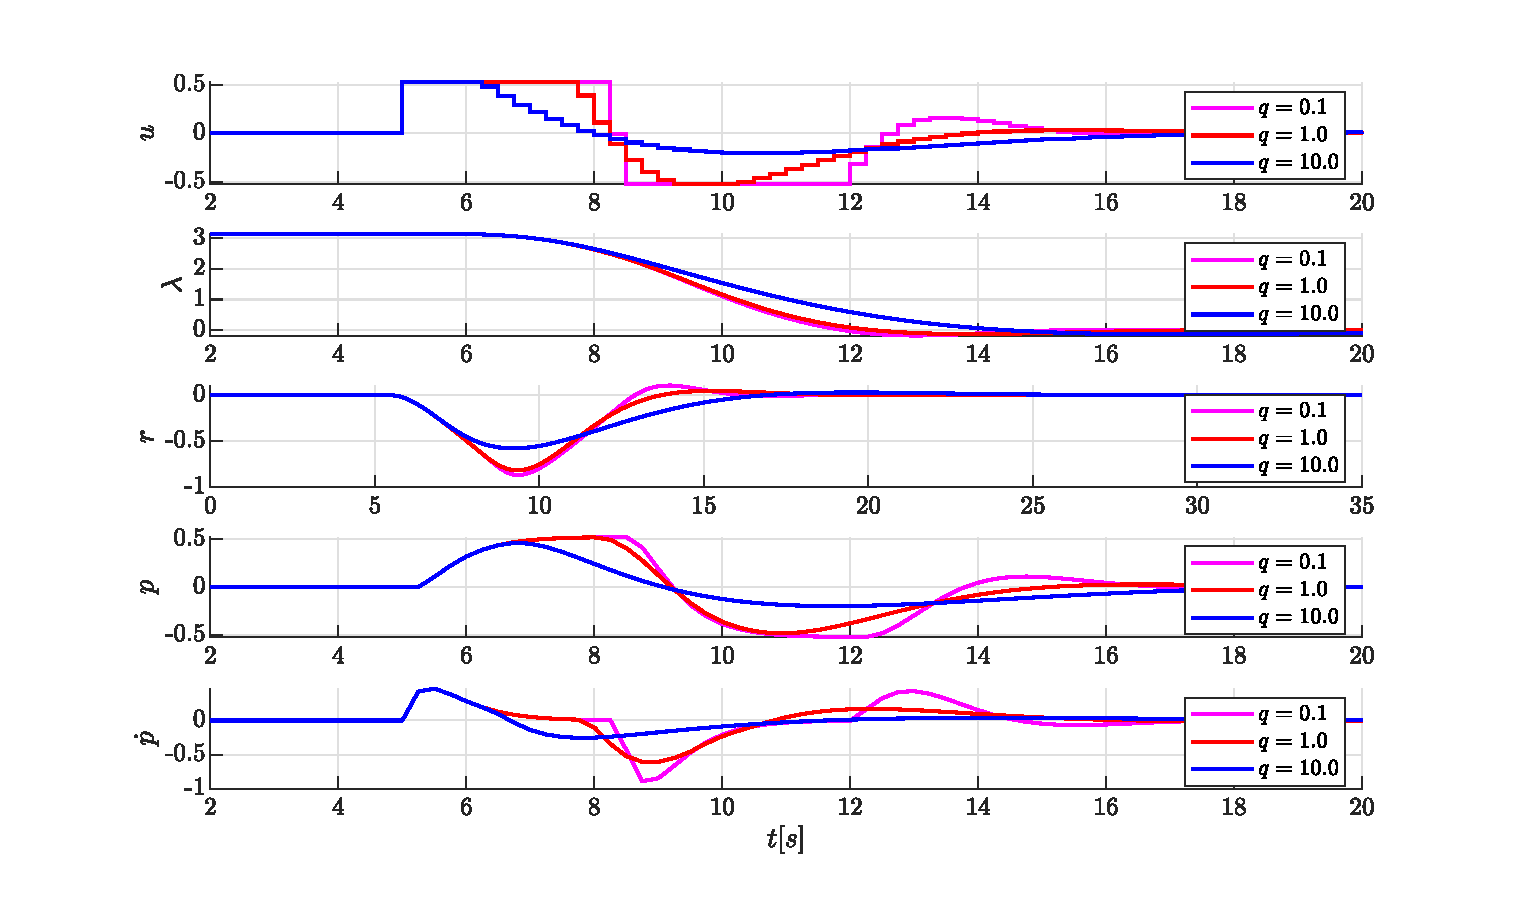
\includegraphics[width=\linewidth]{figures/lab2_optimal_u}
	\caption{Manipulated variable and outputs with different values of $q$.}
	\label{fig:lab2optimalu}
\end{figure}

\subsection{The objective function}
\textit{Furthermore, discuss the objective function (15) (in the lab assignment text) in particular the term $(\lambda_i-\lambda_f )^2$. For instance, could any unwanted effects arise from steering the helicopter to $\lambda =\lambda_f$ with this objective function?}

From the forum: Here are some questions that will help you figure out what is asked for:
What will happen when you have some elements that are very large compared to others in a quadratic objective function? Which consequence(s) does this have for the setup in the lab? What is the impact of the length of the control horizon (imagine that the step length, h, is fixed)?

\clearpage
\subsection{Experimental results}
\textit{Printouts of data from relevant experiments (plots).
Discussion and analysis of the results.
Answer 10.2.2.7 here.}

\begin{figure}[h]
    \begin{center}
        %% Creator: Matplotlib, PGF backend
%%
%% To include the figure in your LaTeX document, write
%%   \input{<filename>.pgf}
%%
%% Make sure the required packages are loaded in your preamble
%%   \usepackage{pgf}
%%
%% and, on pdftex
%%   \usepackage[utf8]{inputenc}\DeclareUnicodeCharacter{2212}{-}
%%
%% or, on luatex and xetex
%%   \usepackage{unicode-math}
%%
%% Figures using additional raster images can only be included by \input if
%% they are in the same directory as the main LaTeX file. For loading figures
%% from other directories you can use the `import` package
%%   \usepackage{import}
%%
%% and then include the figures with
%%   \import{<path to file>}{<filename>.pgf}
%%
%% Matplotlib used the following preamble
%%
\begingroup%
\makeatletter%
\begin{pgfpicture}%
\pgfpathrectangle{\pgfpointorigin}{\pgfqpoint{6.400000in}{4.800000in}}%
\pgfusepath{use as bounding box, clip}%
\begin{pgfscope}%
\pgfsetbuttcap%
\pgfsetmiterjoin%
\definecolor{currentfill}{rgb}{1.000000,1.000000,1.000000}%
\pgfsetfillcolor{currentfill}%
\pgfsetlinewidth{0.000000pt}%
\definecolor{currentstroke}{rgb}{1.000000,1.000000,1.000000}%
\pgfsetstrokecolor{currentstroke}%
\pgfsetdash{}{0pt}%
\pgfpathmoveto{\pgfqpoint{0.000000in}{0.000000in}}%
\pgfpathlineto{\pgfqpoint{6.400000in}{0.000000in}}%
\pgfpathlineto{\pgfqpoint{6.400000in}{4.800000in}}%
\pgfpathlineto{\pgfqpoint{0.000000in}{4.800000in}}%
\pgfpathclose%
\pgfusepath{fill}%
\end{pgfscope}%
\begin{pgfscope}%
\pgfsetbuttcap%
\pgfsetmiterjoin%
\definecolor{currentfill}{rgb}{1.000000,1.000000,1.000000}%
\pgfsetfillcolor{currentfill}%
\pgfsetlinewidth{0.000000pt}%
\definecolor{currentstroke}{rgb}{0.000000,0.000000,0.000000}%
\pgfsetstrokecolor{currentstroke}%
\pgfsetstrokeopacity{0.000000}%
\pgfsetdash{}{0pt}%
\pgfpathmoveto{\pgfqpoint{0.711729in}{2.597338in}}%
\pgfpathlineto{\pgfqpoint{6.180555in}{2.597338in}}%
\pgfpathlineto{\pgfqpoint{6.180555in}{4.285108in}}%
\pgfpathlineto{\pgfqpoint{0.711729in}{4.285108in}}%
\pgfpathclose%
\pgfusepath{fill}%
\end{pgfscope}%
\begin{pgfscope}%
\pgfsetbuttcap%
\pgfsetroundjoin%
\definecolor{currentfill}{rgb}{0.000000,0.000000,0.000000}%
\pgfsetfillcolor{currentfill}%
\pgfsetlinewidth{0.803000pt}%
\definecolor{currentstroke}{rgb}{0.000000,0.000000,0.000000}%
\pgfsetstrokecolor{currentstroke}%
\pgfsetdash{}{0pt}%
\pgfsys@defobject{currentmarker}{\pgfqpoint{0.000000in}{-0.048611in}}{\pgfqpoint{0.000000in}{0.000000in}}{%
\pgfpathmoveto{\pgfqpoint{0.000000in}{0.000000in}}%
\pgfpathlineto{\pgfqpoint{0.000000in}{-0.048611in}}%
\pgfusepath{stroke,fill}%
}%
\begin{pgfscope}%
\pgfsys@transformshift{0.711729in}{2.597338in}%
\pgfsys@useobject{currentmarker}{}%
\end{pgfscope}%
\end{pgfscope}%
\begin{pgfscope}%
\pgfsetbuttcap%
\pgfsetroundjoin%
\definecolor{currentfill}{rgb}{0.000000,0.000000,0.000000}%
\pgfsetfillcolor{currentfill}%
\pgfsetlinewidth{0.803000pt}%
\definecolor{currentstroke}{rgb}{0.000000,0.000000,0.000000}%
\pgfsetstrokecolor{currentstroke}%
\pgfsetdash{}{0pt}%
\pgfsys@defobject{currentmarker}{\pgfqpoint{0.000000in}{-0.048611in}}{\pgfqpoint{0.000000in}{0.000000in}}{%
\pgfpathmoveto{\pgfqpoint{0.000000in}{0.000000in}}%
\pgfpathlineto{\pgfqpoint{0.000000in}{-0.048611in}}%
\pgfusepath{stroke,fill}%
}%
\begin{pgfscope}%
\pgfsys@transformshift{1.623200in}{2.597338in}%
\pgfsys@useobject{currentmarker}{}%
\end{pgfscope}%
\end{pgfscope}%
\begin{pgfscope}%
\pgfsetbuttcap%
\pgfsetroundjoin%
\definecolor{currentfill}{rgb}{0.000000,0.000000,0.000000}%
\pgfsetfillcolor{currentfill}%
\pgfsetlinewidth{0.803000pt}%
\definecolor{currentstroke}{rgb}{0.000000,0.000000,0.000000}%
\pgfsetstrokecolor{currentstroke}%
\pgfsetdash{}{0pt}%
\pgfsys@defobject{currentmarker}{\pgfqpoint{0.000000in}{-0.048611in}}{\pgfqpoint{0.000000in}{0.000000in}}{%
\pgfpathmoveto{\pgfqpoint{0.000000in}{0.000000in}}%
\pgfpathlineto{\pgfqpoint{0.000000in}{-0.048611in}}%
\pgfusepath{stroke,fill}%
}%
\begin{pgfscope}%
\pgfsys@transformshift{2.534671in}{2.597338in}%
\pgfsys@useobject{currentmarker}{}%
\end{pgfscope}%
\end{pgfscope}%
\begin{pgfscope}%
\pgfsetbuttcap%
\pgfsetroundjoin%
\definecolor{currentfill}{rgb}{0.000000,0.000000,0.000000}%
\pgfsetfillcolor{currentfill}%
\pgfsetlinewidth{0.803000pt}%
\definecolor{currentstroke}{rgb}{0.000000,0.000000,0.000000}%
\pgfsetstrokecolor{currentstroke}%
\pgfsetdash{}{0pt}%
\pgfsys@defobject{currentmarker}{\pgfqpoint{0.000000in}{-0.048611in}}{\pgfqpoint{0.000000in}{0.000000in}}{%
\pgfpathmoveto{\pgfqpoint{0.000000in}{0.000000in}}%
\pgfpathlineto{\pgfqpoint{0.000000in}{-0.048611in}}%
\pgfusepath{stroke,fill}%
}%
\begin{pgfscope}%
\pgfsys@transformshift{3.446142in}{2.597338in}%
\pgfsys@useobject{currentmarker}{}%
\end{pgfscope}%
\end{pgfscope}%
\begin{pgfscope}%
\pgfsetbuttcap%
\pgfsetroundjoin%
\definecolor{currentfill}{rgb}{0.000000,0.000000,0.000000}%
\pgfsetfillcolor{currentfill}%
\pgfsetlinewidth{0.803000pt}%
\definecolor{currentstroke}{rgb}{0.000000,0.000000,0.000000}%
\pgfsetstrokecolor{currentstroke}%
\pgfsetdash{}{0pt}%
\pgfsys@defobject{currentmarker}{\pgfqpoint{0.000000in}{-0.048611in}}{\pgfqpoint{0.000000in}{0.000000in}}{%
\pgfpathmoveto{\pgfqpoint{0.000000in}{0.000000in}}%
\pgfpathlineto{\pgfqpoint{0.000000in}{-0.048611in}}%
\pgfusepath{stroke,fill}%
}%
\begin{pgfscope}%
\pgfsys@transformshift{4.357613in}{2.597338in}%
\pgfsys@useobject{currentmarker}{}%
\end{pgfscope}%
\end{pgfscope}%
\begin{pgfscope}%
\pgfsetbuttcap%
\pgfsetroundjoin%
\definecolor{currentfill}{rgb}{0.000000,0.000000,0.000000}%
\pgfsetfillcolor{currentfill}%
\pgfsetlinewidth{0.803000pt}%
\definecolor{currentstroke}{rgb}{0.000000,0.000000,0.000000}%
\pgfsetstrokecolor{currentstroke}%
\pgfsetdash{}{0pt}%
\pgfsys@defobject{currentmarker}{\pgfqpoint{0.000000in}{-0.048611in}}{\pgfqpoint{0.000000in}{0.000000in}}{%
\pgfpathmoveto{\pgfqpoint{0.000000in}{0.000000in}}%
\pgfpathlineto{\pgfqpoint{0.000000in}{-0.048611in}}%
\pgfusepath{stroke,fill}%
}%
\begin{pgfscope}%
\pgfsys@transformshift{5.269084in}{2.597338in}%
\pgfsys@useobject{currentmarker}{}%
\end{pgfscope}%
\end{pgfscope}%
\begin{pgfscope}%
\pgfsetbuttcap%
\pgfsetroundjoin%
\definecolor{currentfill}{rgb}{0.000000,0.000000,0.000000}%
\pgfsetfillcolor{currentfill}%
\pgfsetlinewidth{0.803000pt}%
\definecolor{currentstroke}{rgb}{0.000000,0.000000,0.000000}%
\pgfsetstrokecolor{currentstroke}%
\pgfsetdash{}{0pt}%
\pgfsys@defobject{currentmarker}{\pgfqpoint{0.000000in}{-0.048611in}}{\pgfqpoint{0.000000in}{0.000000in}}{%
\pgfpathmoveto{\pgfqpoint{0.000000in}{0.000000in}}%
\pgfpathlineto{\pgfqpoint{0.000000in}{-0.048611in}}%
\pgfusepath{stroke,fill}%
}%
\begin{pgfscope}%
\pgfsys@transformshift{6.180555in}{2.597338in}%
\pgfsys@useobject{currentmarker}{}%
\end{pgfscope}%
\end{pgfscope}%
\begin{pgfscope}%
\definecolor{textcolor}{rgb}{0.000000,0.000000,0.000000}%
\pgfsetstrokecolor{textcolor}%
\pgfsetfillcolor{textcolor}%
\pgftext[x=3.446142in,y=2.541782in,,top]{\color{textcolor}\rmfamily\fontsize{10.000000}{12.000000}\selectfont Time [s]}%
\end{pgfscope}%
\begin{pgfscope}%
\pgfsetbuttcap%
\pgfsetroundjoin%
\definecolor{currentfill}{rgb}{0.000000,0.000000,0.000000}%
\pgfsetfillcolor{currentfill}%
\pgfsetlinewidth{0.803000pt}%
\definecolor{currentstroke}{rgb}{0.000000,0.000000,0.000000}%
\pgfsetstrokecolor{currentstroke}%
\pgfsetdash{}{0pt}%
\pgfsys@defobject{currentmarker}{\pgfqpoint{-0.048611in}{0.000000in}}{\pgfqpoint{-0.000000in}{0.000000in}}{%
\pgfpathmoveto{\pgfqpoint{-0.000000in}{0.000000in}}%
\pgfpathlineto{\pgfqpoint{-0.048611in}{0.000000in}}%
\pgfusepath{stroke,fill}%
}%
\begin{pgfscope}%
\pgfsys@transformshift{0.711729in}{2.597338in}%
\pgfsys@useobject{currentmarker}{}%
\end{pgfscope}%
\end{pgfscope}%
\begin{pgfscope}%
\definecolor{textcolor}{rgb}{0.000000,0.000000,0.000000}%
\pgfsetstrokecolor{textcolor}%
\pgfsetfillcolor{textcolor}%
\pgftext[x=0.545062in, y=2.549113in, left, base]{\color{textcolor}\rmfamily\fontsize{10.000000}{12.000000}\selectfont \(\displaystyle {0}\)}%
\end{pgfscope}%
\begin{pgfscope}%
\pgfsetbuttcap%
\pgfsetroundjoin%
\definecolor{currentfill}{rgb}{0.000000,0.000000,0.000000}%
\pgfsetfillcolor{currentfill}%
\pgfsetlinewidth{0.803000pt}%
\definecolor{currentstroke}{rgb}{0.000000,0.000000,0.000000}%
\pgfsetstrokecolor{currentstroke}%
\pgfsetdash{}{0pt}%
\pgfsys@defobject{currentmarker}{\pgfqpoint{-0.048611in}{0.000000in}}{\pgfqpoint{-0.000000in}{0.000000in}}{%
\pgfpathmoveto{\pgfqpoint{-0.000000in}{0.000000in}}%
\pgfpathlineto{\pgfqpoint{-0.048611in}{0.000000in}}%
\pgfusepath{stroke,fill}%
}%
\begin{pgfscope}%
\pgfsys@transformshift{0.711729in}{2.934892in}%
\pgfsys@useobject{currentmarker}{}%
\end{pgfscope}%
\end{pgfscope}%
\begin{pgfscope}%
\definecolor{textcolor}{rgb}{0.000000,0.000000,0.000000}%
\pgfsetstrokecolor{textcolor}%
\pgfsetfillcolor{textcolor}%
\pgftext[x=0.545062in, y=2.886667in, left, base]{\color{textcolor}\rmfamily\fontsize{10.000000}{12.000000}\selectfont \(\displaystyle {1}\)}%
\end{pgfscope}%
\begin{pgfscope}%
\pgfsetbuttcap%
\pgfsetroundjoin%
\definecolor{currentfill}{rgb}{0.000000,0.000000,0.000000}%
\pgfsetfillcolor{currentfill}%
\pgfsetlinewidth{0.803000pt}%
\definecolor{currentstroke}{rgb}{0.000000,0.000000,0.000000}%
\pgfsetstrokecolor{currentstroke}%
\pgfsetdash{}{0pt}%
\pgfsys@defobject{currentmarker}{\pgfqpoint{-0.048611in}{0.000000in}}{\pgfqpoint{-0.000000in}{0.000000in}}{%
\pgfpathmoveto{\pgfqpoint{-0.000000in}{0.000000in}}%
\pgfpathlineto{\pgfqpoint{-0.048611in}{0.000000in}}%
\pgfusepath{stroke,fill}%
}%
\begin{pgfscope}%
\pgfsys@transformshift{0.711729in}{3.272446in}%
\pgfsys@useobject{currentmarker}{}%
\end{pgfscope}%
\end{pgfscope}%
\begin{pgfscope}%
\definecolor{textcolor}{rgb}{0.000000,0.000000,0.000000}%
\pgfsetstrokecolor{textcolor}%
\pgfsetfillcolor{textcolor}%
\pgftext[x=0.545062in, y=3.224221in, left, base]{\color{textcolor}\rmfamily\fontsize{10.000000}{12.000000}\selectfont \(\displaystyle {2}\)}%
\end{pgfscope}%
\begin{pgfscope}%
\pgfsetbuttcap%
\pgfsetroundjoin%
\definecolor{currentfill}{rgb}{0.000000,0.000000,0.000000}%
\pgfsetfillcolor{currentfill}%
\pgfsetlinewidth{0.803000pt}%
\definecolor{currentstroke}{rgb}{0.000000,0.000000,0.000000}%
\pgfsetstrokecolor{currentstroke}%
\pgfsetdash{}{0pt}%
\pgfsys@defobject{currentmarker}{\pgfqpoint{-0.048611in}{0.000000in}}{\pgfqpoint{-0.000000in}{0.000000in}}{%
\pgfpathmoveto{\pgfqpoint{-0.000000in}{0.000000in}}%
\pgfpathlineto{\pgfqpoint{-0.048611in}{0.000000in}}%
\pgfusepath{stroke,fill}%
}%
\begin{pgfscope}%
\pgfsys@transformshift{0.711729in}{3.610000in}%
\pgfsys@useobject{currentmarker}{}%
\end{pgfscope}%
\end{pgfscope}%
\begin{pgfscope}%
\definecolor{textcolor}{rgb}{0.000000,0.000000,0.000000}%
\pgfsetstrokecolor{textcolor}%
\pgfsetfillcolor{textcolor}%
\pgftext[x=0.545062in, y=3.561775in, left, base]{\color{textcolor}\rmfamily\fontsize{10.000000}{12.000000}\selectfont \(\displaystyle {3}\)}%
\end{pgfscope}%
\begin{pgfscope}%
\pgfsetbuttcap%
\pgfsetroundjoin%
\definecolor{currentfill}{rgb}{0.000000,0.000000,0.000000}%
\pgfsetfillcolor{currentfill}%
\pgfsetlinewidth{0.803000pt}%
\definecolor{currentstroke}{rgb}{0.000000,0.000000,0.000000}%
\pgfsetstrokecolor{currentstroke}%
\pgfsetdash{}{0pt}%
\pgfsys@defobject{currentmarker}{\pgfqpoint{-0.048611in}{0.000000in}}{\pgfqpoint{-0.000000in}{0.000000in}}{%
\pgfpathmoveto{\pgfqpoint{-0.000000in}{0.000000in}}%
\pgfpathlineto{\pgfqpoint{-0.048611in}{0.000000in}}%
\pgfusepath{stroke,fill}%
}%
\begin{pgfscope}%
\pgfsys@transformshift{0.711729in}{3.947554in}%
\pgfsys@useobject{currentmarker}{}%
\end{pgfscope}%
\end{pgfscope}%
\begin{pgfscope}%
\definecolor{textcolor}{rgb}{0.000000,0.000000,0.000000}%
\pgfsetstrokecolor{textcolor}%
\pgfsetfillcolor{textcolor}%
\pgftext[x=0.545062in, y=3.899329in, left, base]{\color{textcolor}\rmfamily\fontsize{10.000000}{12.000000}\selectfont \(\displaystyle {4}\)}%
\end{pgfscope}%
\begin{pgfscope}%
\pgfsetbuttcap%
\pgfsetroundjoin%
\definecolor{currentfill}{rgb}{0.000000,0.000000,0.000000}%
\pgfsetfillcolor{currentfill}%
\pgfsetlinewidth{0.803000pt}%
\definecolor{currentstroke}{rgb}{0.000000,0.000000,0.000000}%
\pgfsetstrokecolor{currentstroke}%
\pgfsetdash{}{0pt}%
\pgfsys@defobject{currentmarker}{\pgfqpoint{-0.048611in}{0.000000in}}{\pgfqpoint{-0.000000in}{0.000000in}}{%
\pgfpathmoveto{\pgfqpoint{-0.000000in}{0.000000in}}%
\pgfpathlineto{\pgfqpoint{-0.048611in}{0.000000in}}%
\pgfusepath{stroke,fill}%
}%
\begin{pgfscope}%
\pgfsys@transformshift{0.711729in}{4.285108in}%
\pgfsys@useobject{currentmarker}{}%
\end{pgfscope}%
\end{pgfscope}%
\begin{pgfscope}%
\definecolor{textcolor}{rgb}{0.000000,0.000000,0.000000}%
\pgfsetstrokecolor{textcolor}%
\pgfsetfillcolor{textcolor}%
\pgftext[x=0.545062in, y=4.236883in, left, base]{\color{textcolor}\rmfamily\fontsize{10.000000}{12.000000}\selectfont \(\displaystyle {5}\)}%
\end{pgfscope}%
\begin{pgfscope}%
\definecolor{textcolor}{rgb}{0.000000,0.000000,0.000000}%
\pgfsetstrokecolor{textcolor}%
\pgfsetfillcolor{textcolor}%
\pgftext[x=0.489507in,y=3.441223in,,bottom,rotate=90.000000]{\color{textcolor}\rmfamily\fontsize{10.000000}{12.000000}\selectfont Rad}%
\end{pgfscope}%
\begin{pgfscope}%
\pgfpathrectangle{\pgfqpoint{0.711729in}{2.597338in}}{\pgfqpoint{5.468826in}{1.687770in}}%
\pgfusepath{clip}%
\pgfsetrectcap%
\pgfsetroundjoin%
\pgfsetlinewidth{1.505625pt}%
\definecolor{currentstroke}{rgb}{0.121569,0.466667,0.705882}%
\pgfsetstrokecolor{currentstroke}%
\pgfsetdash{}{0pt}%
\pgfpathmoveto{\pgfqpoint{0.711729in}{3.657795in}}%
\pgfpathlineto{\pgfqpoint{0.750376in}{3.658831in}}%
\pgfpathlineto{\pgfqpoint{0.752563in}{3.659090in}}%
\pgfpathlineto{\pgfqpoint{0.766053in}{3.660125in}}%
\pgfpathlineto{\pgfqpoint{0.768240in}{3.660384in}}%
\pgfpathlineto{\pgfqpoint{0.777720in}{3.661420in}}%
\pgfpathlineto{\pgfqpoint{0.780272in}{3.661938in}}%
\pgfpathlineto{\pgfqpoint{0.789022in}{3.662714in}}%
\pgfpathlineto{\pgfqpoint{0.790116in}{3.663232in}}%
\pgfpathlineto{\pgfqpoint{0.790480in}{3.662973in}}%
\pgfpathlineto{\pgfqpoint{0.795949in}{3.663750in}}%
\pgfpathlineto{\pgfqpoint{0.797043in}{3.664268in}}%
\pgfpathlineto{\pgfqpoint{0.797407in}{3.664009in}}%
\pgfpathlineto{\pgfqpoint{0.798137in}{3.664009in}}%
\pgfpathlineto{\pgfqpoint{0.798501in}{3.664527in}}%
\pgfpathlineto{\pgfqpoint{0.809074in}{3.665562in}}%
\pgfpathlineto{\pgfqpoint{0.811626in}{3.666080in}}%
\pgfpathlineto{\pgfqpoint{0.819283in}{3.667116in}}%
\pgfpathlineto{\pgfqpoint{0.821835in}{3.667633in}}%
\pgfpathlineto{\pgfqpoint{0.830585in}{3.668669in}}%
\pgfpathlineto{\pgfqpoint{0.833137in}{3.669187in}}%
\pgfpathlineto{\pgfqpoint{0.841523in}{3.670222in}}%
\pgfpathlineto{\pgfqpoint{0.844075in}{3.670740in}}%
\pgfpathlineto{\pgfqpoint{0.852096in}{3.671776in}}%
\pgfpathlineto{\pgfqpoint{0.854648in}{3.672294in}}%
\pgfpathlineto{\pgfqpoint{0.863763in}{3.673329in}}%
\pgfpathlineto{\pgfqpoint{0.866315in}{3.673847in}}%
\pgfpathlineto{\pgfqpoint{0.875794in}{3.674883in}}%
\pgfpathlineto{\pgfqpoint{0.878346in}{3.675400in}}%
\pgfpathlineto{\pgfqpoint{0.887825in}{3.676436in}}%
\pgfpathlineto{\pgfqpoint{0.890013in}{3.676695in}}%
\pgfpathlineto{\pgfqpoint{0.898034in}{3.677731in}}%
\pgfpathlineto{\pgfqpoint{0.900586in}{3.678248in}}%
\pgfpathlineto{\pgfqpoint{0.910794in}{3.679284in}}%
\pgfpathlineto{\pgfqpoint{0.913347in}{3.679802in}}%
\pgfpathlineto{\pgfqpoint{0.923190in}{3.680837in}}%
\pgfpathlineto{\pgfqpoint{0.925378in}{3.681096in}}%
\pgfpathlineto{\pgfqpoint{0.934128in}{3.682132in}}%
\pgfpathlineto{\pgfqpoint{0.936680in}{3.682650in}}%
\pgfpathlineto{\pgfqpoint{0.946889in}{3.683685in}}%
\pgfpathlineto{\pgfqpoint{0.949441in}{3.684203in}}%
\pgfpathlineto{\pgfqpoint{0.958920in}{3.685239in}}%
\pgfpathlineto{\pgfqpoint{0.961472in}{3.685756in}}%
\pgfpathlineto{\pgfqpoint{0.970952in}{3.686792in}}%
\pgfpathlineto{\pgfqpoint{0.973504in}{3.687310in}}%
\pgfpathlineto{\pgfqpoint{0.982618in}{3.688345in}}%
\pgfpathlineto{\pgfqpoint{0.985170in}{3.688863in}}%
\pgfpathlineto{\pgfqpoint{0.993921in}{3.689899in}}%
\pgfpathlineto{\pgfqpoint{0.996473in}{3.690417in}}%
\pgfpathlineto{\pgfqpoint{1.004858in}{3.691452in}}%
\pgfpathlineto{\pgfqpoint{1.007410in}{3.691970in}}%
\pgfpathlineto{\pgfqpoint{1.015431in}{3.693006in}}%
\pgfpathlineto{\pgfqpoint{1.017983in}{3.693523in}}%
\pgfpathlineto{\pgfqpoint{1.026004in}{3.694559in}}%
\pgfpathlineto{\pgfqpoint{1.028556in}{3.695077in}}%
\pgfpathlineto{\pgfqpoint{1.035484in}{3.696112in}}%
\pgfpathlineto{\pgfqpoint{1.038036in}{3.696630in}}%
\pgfpathlineto{\pgfqpoint{1.044963in}{3.697666in}}%
\pgfpathlineto{\pgfqpoint{1.047515in}{3.698184in}}%
\pgfpathlineto{\pgfqpoint{1.054078in}{3.699219in}}%
\pgfpathlineto{\pgfqpoint{1.056630in}{3.699737in}}%
\pgfpathlineto{\pgfqpoint{1.063557in}{3.700773in}}%
\pgfpathlineto{\pgfqpoint{1.066109in}{3.701290in}}%
\pgfpathlineto{\pgfqpoint{1.072307in}{3.702326in}}%
\pgfpathlineto{\pgfqpoint{1.075224in}{3.703103in}}%
\pgfpathlineto{\pgfqpoint{1.082151in}{3.704138in}}%
\pgfpathlineto{\pgfqpoint{1.084703in}{3.704656in}}%
\pgfpathlineto{\pgfqpoint{1.090537in}{3.705692in}}%
\pgfpathlineto{\pgfqpoint{1.093453in}{3.706469in}}%
\pgfpathlineto{\pgfqpoint{1.100016in}{3.707504in}}%
\pgfpathlineto{\pgfqpoint{1.102568in}{3.708022in}}%
\pgfpathlineto{\pgfqpoint{1.108401in}{3.709058in}}%
\pgfpathlineto{\pgfqpoint{1.111318in}{3.709834in}}%
\pgfpathlineto{\pgfqpoint{1.117881in}{3.710870in}}%
\pgfpathlineto{\pgfqpoint{1.120797in}{3.711647in}}%
\pgfpathlineto{\pgfqpoint{1.126995in}{3.712682in}}%
\pgfpathlineto{\pgfqpoint{1.129912in}{3.713459in}}%
\pgfpathlineto{\pgfqpoint{1.135745in}{3.714494in}}%
\pgfpathlineto{\pgfqpoint{1.138662in}{3.715271in}}%
\pgfpathlineto{\pgfqpoint{1.144860in}{3.716307in}}%
\pgfpathlineto{\pgfqpoint{1.147777in}{3.717083in}}%
\pgfpathlineto{\pgfqpoint{1.153610in}{3.718119in}}%
\pgfpathlineto{\pgfqpoint{1.156527in}{3.718896in}}%
\pgfpathlineto{\pgfqpoint{1.162360in}{3.719931in}}%
\pgfpathlineto{\pgfqpoint{1.165277in}{3.720708in}}%
\pgfpathlineto{\pgfqpoint{1.170381in}{3.721744in}}%
\pgfpathlineto{\pgfqpoint{1.173298in}{3.722520in}}%
\pgfpathlineto{\pgfqpoint{1.179132in}{3.723556in}}%
\pgfpathlineto{\pgfqpoint{1.182048in}{3.724333in}}%
\pgfpathlineto{\pgfqpoint{1.187517in}{3.725368in}}%
\pgfpathlineto{\pgfqpoint{1.190434in}{3.726145in}}%
\pgfpathlineto{\pgfqpoint{1.195903in}{3.727181in}}%
\pgfpathlineto{\pgfqpoint{1.198819in}{3.727957in}}%
\pgfpathlineto{\pgfqpoint{1.203924in}{3.728993in}}%
\pgfpathlineto{\pgfqpoint{1.206840in}{3.729770in}}%
\pgfpathlineto{\pgfqpoint{1.211580in}{3.730805in}}%
\pgfpathlineto{\pgfqpoint{1.214497in}{3.731582in}}%
\pgfpathlineto{\pgfqpoint{1.219601in}{3.732617in}}%
\pgfpathlineto{\pgfqpoint{1.222518in}{3.733394in}}%
\pgfpathlineto{\pgfqpoint{1.227622in}{3.734430in}}%
\pgfpathlineto{\pgfqpoint{1.230538in}{3.735206in}}%
\pgfpathlineto{\pgfqpoint{1.235278in}{3.736242in}}%
\pgfpathlineto{\pgfqpoint{1.238559in}{3.737278in}}%
\pgfpathlineto{\pgfqpoint{1.243664in}{3.738313in}}%
\pgfpathlineto{\pgfqpoint{1.246580in}{3.739090in}}%
\pgfpathlineto{\pgfqpoint{1.251320in}{3.740126in}}%
\pgfpathlineto{\pgfqpoint{1.254237in}{3.740902in}}%
\pgfpathlineto{\pgfqpoint{1.258612in}{3.741938in}}%
\pgfpathlineto{\pgfqpoint{1.261528in}{3.742715in}}%
\pgfpathlineto{\pgfqpoint{1.266268in}{3.743750in}}%
\pgfpathlineto{\pgfqpoint{1.269185in}{3.744527in}}%
\pgfpathlineto{\pgfqpoint{1.273560in}{3.745563in}}%
\pgfpathlineto{\pgfqpoint{1.276477in}{3.746339in}}%
\pgfpathlineto{\pgfqpoint{1.280852in}{3.747375in}}%
\pgfpathlineto{\pgfqpoint{1.284133in}{3.748410in}}%
\pgfpathlineto{\pgfqpoint{1.288873in}{3.749446in}}%
\pgfpathlineto{\pgfqpoint{1.292154in}{3.750482in}}%
\pgfpathlineto{\pgfqpoint{1.296894in}{3.751517in}}%
\pgfpathlineto{\pgfqpoint{1.299810in}{3.752294in}}%
\pgfpathlineto{\pgfqpoint{1.303821in}{3.753330in}}%
\pgfpathlineto{\pgfqpoint{1.306737in}{3.754106in}}%
\pgfpathlineto{\pgfqpoint{1.310748in}{3.755142in}}%
\pgfpathlineto{\pgfqpoint{1.313665in}{3.755919in}}%
\pgfpathlineto{\pgfqpoint{1.317675in}{3.756954in}}%
\pgfpathlineto{\pgfqpoint{1.320592in}{3.757731in}}%
\pgfpathlineto{\pgfqpoint{1.324602in}{3.758766in}}%
\pgfpathlineto{\pgfqpoint{1.327884in}{3.759802in}}%
\pgfpathlineto{\pgfqpoint{1.332259in}{3.760838in}}%
\pgfpathlineto{\pgfqpoint{1.335175in}{3.761614in}}%
\pgfpathlineto{\pgfqpoint{1.339186in}{3.762650in}}%
\pgfpathlineto{\pgfqpoint{1.342467in}{3.763686in}}%
\pgfpathlineto{\pgfqpoint{1.346842in}{3.764721in}}%
\pgfpathlineto{\pgfqpoint{1.350123in}{3.765757in}}%
\pgfpathlineto{\pgfqpoint{1.354499in}{3.766792in}}%
\pgfpathlineto{\pgfqpoint{1.357780in}{3.767828in}}%
\pgfpathlineto{\pgfqpoint{1.361790in}{3.768864in}}%
\pgfpathlineto{\pgfqpoint{1.365072in}{3.769899in}}%
\pgfpathlineto{\pgfqpoint{1.369447in}{3.770935in}}%
\pgfpathlineto{\pgfqpoint{1.372728in}{3.771970in}}%
\pgfpathlineto{\pgfqpoint{1.376738in}{3.773006in}}%
\pgfpathlineto{\pgfqpoint{1.380020in}{3.774042in}}%
\pgfpathlineto{\pgfqpoint{1.384030in}{3.775077in}}%
\pgfpathlineto{\pgfqpoint{1.387311in}{3.776113in}}%
\pgfpathlineto{\pgfqpoint{1.391322in}{3.777148in}}%
\pgfpathlineto{\pgfqpoint{1.394603in}{3.778184in}}%
\pgfpathlineto{\pgfqpoint{1.398614in}{3.779220in}}%
\pgfpathlineto{\pgfqpoint{1.401895in}{3.780255in}}%
\pgfpathlineto{\pgfqpoint{1.405541in}{3.781291in}}%
\pgfpathlineto{\pgfqpoint{1.408822in}{3.782326in}}%
\pgfpathlineto{\pgfqpoint{1.412468in}{3.783362in}}%
\pgfpathlineto{\pgfqpoint{1.415385in}{3.784139in}}%
\pgfpathlineto{\pgfqpoint{1.419031in}{3.785174in}}%
\pgfpathlineto{\pgfqpoint{1.422312in}{3.786210in}}%
\pgfpathlineto{\pgfqpoint{1.425958in}{3.787246in}}%
\pgfpathlineto{\pgfqpoint{1.429239in}{3.788281in}}%
\pgfpathlineto{\pgfqpoint{1.432885in}{3.789317in}}%
\pgfpathlineto{\pgfqpoint{1.436166in}{3.790352in}}%
\pgfpathlineto{\pgfqpoint{1.439812in}{3.791388in}}%
\pgfpathlineto{\pgfqpoint{1.443094in}{3.792424in}}%
\pgfpathlineto{\pgfqpoint{1.446739in}{3.793459in}}%
\pgfpathlineto{\pgfqpoint{1.450021in}{3.794495in}}%
\pgfpathlineto{\pgfqpoint{1.453667in}{3.795530in}}%
\pgfpathlineto{\pgfqpoint{1.457312in}{3.796825in}}%
\pgfpathlineto{\pgfqpoint{1.461323in}{3.797860in}}%
\pgfpathlineto{\pgfqpoint{1.464969in}{3.799155in}}%
\pgfpathlineto{\pgfqpoint{1.468979in}{3.800191in}}%
\pgfpathlineto{\pgfqpoint{1.472625in}{3.801485in}}%
\pgfpathlineto{\pgfqpoint{1.476271in}{3.802521in}}%
\pgfpathlineto{\pgfqpoint{1.479917in}{3.803815in}}%
\pgfpathlineto{\pgfqpoint{1.483563in}{3.804851in}}%
\pgfpathlineto{\pgfqpoint{1.486844in}{3.805886in}}%
\pgfpathlineto{\pgfqpoint{1.490490in}{3.806922in}}%
\pgfpathlineto{\pgfqpoint{1.494136in}{3.808216in}}%
\pgfpathlineto{\pgfqpoint{1.497782in}{3.809252in}}%
\pgfpathlineto{\pgfqpoint{1.501063in}{3.810288in}}%
\pgfpathlineto{\pgfqpoint{1.504344in}{3.811323in}}%
\pgfpathlineto{\pgfqpoint{1.507990in}{3.812618in}}%
\pgfpathlineto{\pgfqpoint{1.511636in}{3.813653in}}%
\pgfpathlineto{\pgfqpoint{1.515282in}{3.814948in}}%
\pgfpathlineto{\pgfqpoint{1.518563in}{3.815983in}}%
\pgfpathlineto{\pgfqpoint{1.522209in}{3.817278in}}%
\pgfpathlineto{\pgfqpoint{1.525855in}{3.818314in}}%
\pgfpathlineto{\pgfqpoint{1.529501in}{3.819608in}}%
\pgfpathlineto{\pgfqpoint{1.532782in}{3.820644in}}%
\pgfpathlineto{\pgfqpoint{1.536428in}{3.821938in}}%
\pgfpathlineto{\pgfqpoint{1.540074in}{3.822974in}}%
\pgfpathlineto{\pgfqpoint{1.544085in}{3.824527in}}%
\pgfpathlineto{\pgfqpoint{1.547730in}{3.825563in}}%
\pgfpathlineto{\pgfqpoint{1.551741in}{3.827116in}}%
\pgfpathlineto{\pgfqpoint{1.555387in}{3.828152in}}%
\pgfpathlineto{\pgfqpoint{1.559033in}{3.829446in}}%
\pgfpathlineto{\pgfqpoint{1.562314in}{3.830482in}}%
\pgfpathlineto{\pgfqpoint{1.566324in}{3.832035in}}%
\pgfpathlineto{\pgfqpoint{1.569606in}{3.833071in}}%
\pgfpathlineto{\pgfqpoint{1.573252in}{3.834365in}}%
\pgfpathlineto{\pgfqpoint{1.576533in}{3.835401in}}%
\pgfpathlineto{\pgfqpoint{1.580543in}{3.836954in}}%
\pgfpathlineto{\pgfqpoint{1.583825in}{3.837990in}}%
\pgfpathlineto{\pgfqpoint{1.587471in}{3.839285in}}%
\pgfpathlineto{\pgfqpoint{1.590752in}{3.840320in}}%
\pgfpathlineto{\pgfqpoint{1.594762in}{3.841874in}}%
\pgfpathlineto{\pgfqpoint{1.598044in}{3.842909in}}%
\pgfpathlineto{\pgfqpoint{1.602054in}{3.844463in}}%
\pgfpathlineto{\pgfqpoint{1.605335in}{3.845498in}}%
\pgfpathlineto{\pgfqpoint{1.608981in}{3.846793in}}%
\pgfpathlineto{\pgfqpoint{1.611898in}{3.847828in}}%
\pgfpathlineto{\pgfqpoint{1.615908in}{3.849382in}}%
\pgfpathlineto{\pgfqpoint{1.618825in}{3.850417in}}%
\pgfpathlineto{\pgfqpoint{1.622836in}{3.851971in}}%
\pgfpathlineto{\pgfqpoint{1.626481in}{3.853006in}}%
\pgfpathlineto{\pgfqpoint{1.630492in}{3.854560in}}%
\pgfpathlineto{\pgfqpoint{1.633409in}{3.855595in}}%
\pgfpathlineto{\pgfqpoint{1.637419in}{3.857149in}}%
\pgfpathlineto{\pgfqpoint{1.640700in}{3.858184in}}%
\pgfpathlineto{\pgfqpoint{1.644711in}{3.859738in}}%
\pgfpathlineto{\pgfqpoint{1.647992in}{3.860773in}}%
\pgfpathlineto{\pgfqpoint{1.652003in}{3.862327in}}%
\pgfpathlineto{\pgfqpoint{1.655284in}{3.863362in}}%
\pgfpathlineto{\pgfqpoint{1.658930in}{3.864657in}}%
\pgfpathlineto{\pgfqpoint{1.662211in}{3.865692in}}%
\pgfpathlineto{\pgfqpoint{1.665857in}{3.866987in}}%
\pgfpathlineto{\pgfqpoint{1.668774in}{3.868023in}}%
\pgfpathlineto{\pgfqpoint{1.672420in}{3.869317in}}%
\pgfpathlineto{\pgfqpoint{1.675701in}{3.870353in}}%
\pgfpathlineto{\pgfqpoint{1.679347in}{3.871647in}}%
\pgfpathlineto{\pgfqpoint{1.682628in}{3.872683in}}%
\pgfpathlineto{\pgfqpoint{1.685909in}{3.873718in}}%
\pgfpathlineto{\pgfqpoint{1.689191in}{3.874754in}}%
\pgfpathlineto{\pgfqpoint{1.692837in}{3.876048in}}%
\pgfpathlineto{\pgfqpoint{1.696847in}{3.877084in}}%
\pgfpathlineto{\pgfqpoint{1.700128in}{3.878120in}}%
\pgfpathlineto{\pgfqpoint{1.703410in}{3.879155in}}%
\pgfpathlineto{\pgfqpoint{1.706326in}{3.879932in}}%
\pgfpathlineto{\pgfqpoint{1.709972in}{3.880968in}}%
\pgfpathlineto{\pgfqpoint{1.712889in}{3.881744in}}%
\pgfpathlineto{\pgfqpoint{1.716535in}{3.882780in}}%
\pgfpathlineto{\pgfqpoint{1.719452in}{3.883557in}}%
\pgfpathlineto{\pgfqpoint{1.724191in}{3.884592in}}%
\pgfpathlineto{\pgfqpoint{1.727472in}{3.885628in}}%
\pgfpathlineto{\pgfqpoint{1.731848in}{3.886663in}}%
\pgfpathlineto{\pgfqpoint{1.734764in}{3.887440in}}%
\pgfpathlineto{\pgfqpoint{1.740233in}{3.888476in}}%
\pgfpathlineto{\pgfqpoint{1.743150in}{3.889252in}}%
\pgfpathlineto{\pgfqpoint{1.748619in}{3.890288in}}%
\pgfpathlineto{\pgfqpoint{1.751535in}{3.891065in}}%
\pgfpathlineto{\pgfqpoint{1.757733in}{3.892100in}}%
\pgfpathlineto{\pgfqpoint{1.760285in}{3.892618in}}%
\pgfpathlineto{\pgfqpoint{1.766848in}{3.893654in}}%
\pgfpathlineto{\pgfqpoint{1.769765in}{3.894430in}}%
\pgfpathlineto{\pgfqpoint{1.778515in}{3.895466in}}%
\pgfpathlineto{\pgfqpoint{1.781067in}{3.895984in}}%
\pgfpathlineto{\pgfqpoint{1.791640in}{3.897019in}}%
\pgfpathlineto{\pgfqpoint{1.793828in}{3.897278in}}%
\pgfpathlineto{\pgfqpoint{1.806224in}{3.898314in}}%
\pgfpathlineto{\pgfqpoint{1.808411in}{3.898573in}}%
\pgfpathlineto{\pgfqpoint{1.866381in}{3.897537in}}%
\pgfpathlineto{\pgfqpoint{1.868933in}{3.897019in}}%
\pgfpathlineto{\pgfqpoint{1.878047in}{3.895984in}}%
\pgfpathlineto{\pgfqpoint{1.880600in}{3.895466in}}%
\pgfpathlineto{\pgfqpoint{1.888621in}{3.894430in}}%
\pgfpathlineto{\pgfqpoint{1.891537in}{3.893654in}}%
\pgfpathlineto{\pgfqpoint{1.897735in}{3.892618in}}%
\pgfpathlineto{\pgfqpoint{1.900652in}{3.891841in}}%
\pgfpathlineto{\pgfqpoint{1.906121in}{3.890806in}}%
\pgfpathlineto{\pgfqpoint{1.909402in}{3.889770in}}%
\pgfpathlineto{\pgfqpoint{1.914506in}{3.888735in}}%
\pgfpathlineto{\pgfqpoint{1.918152in}{3.887440in}}%
\pgfpathlineto{\pgfqpoint{1.922527in}{3.886404in}}%
\pgfpathlineto{\pgfqpoint{1.925444in}{3.885628in}}%
\pgfpathlineto{\pgfqpoint{1.928725in}{3.884592in}}%
\pgfpathlineto{\pgfqpoint{1.932007in}{3.883557in}}%
\pgfpathlineto{\pgfqpoint{1.935288in}{3.882521in}}%
\pgfpathlineto{\pgfqpoint{1.938934in}{3.881226in}}%
\pgfpathlineto{\pgfqpoint{1.941850in}{3.880191in}}%
\pgfpathlineto{\pgfqpoint{1.945496in}{3.878896in}}%
\pgfpathlineto{\pgfqpoint{1.948413in}{3.877861in}}%
\pgfpathlineto{\pgfqpoint{1.952424in}{3.876307in}}%
\pgfpathlineto{\pgfqpoint{1.954976in}{3.875272in}}%
\pgfpathlineto{\pgfqpoint{1.959715in}{3.873201in}}%
\pgfpathlineto{\pgfqpoint{1.962997in}{3.872165in}}%
\pgfpathlineto{\pgfqpoint{1.968830in}{3.869317in}}%
\pgfpathlineto{\pgfqpoint{1.971747in}{3.868281in}}%
\pgfpathlineto{\pgfqpoint{1.977945in}{3.865175in}}%
\pgfpathlineto{\pgfqpoint{1.980497in}{3.864139in}}%
\pgfpathlineto{\pgfqpoint{1.988518in}{3.859738in}}%
\pgfpathlineto{\pgfqpoint{1.991070in}{3.858702in}}%
\pgfpathlineto{\pgfqpoint{1.999820in}{3.853783in}}%
\pgfpathlineto{\pgfqpoint{2.002008in}{3.852747in}}%
\pgfpathlineto{\pgfqpoint{2.012945in}{3.846275in}}%
\pgfpathlineto{\pgfqpoint{2.014404in}{3.845239in}}%
\pgfpathlineto{\pgfqpoint{2.032268in}{3.833848in}}%
\pgfpathlineto{\pgfqpoint{2.034091in}{3.832812in}}%
\pgfpathlineto{\pgfqpoint{2.072009in}{3.804592in}}%
\pgfpathlineto{\pgfqpoint{2.075290in}{3.801744in}}%
\pgfpathlineto{\pgfqpoint{2.085498in}{3.793200in}}%
\pgfpathlineto{\pgfqpoint{2.088780in}{3.790352in}}%
\pgfpathlineto{\pgfqpoint{2.096436in}{3.783621in}}%
\pgfpathlineto{\pgfqpoint{2.100082in}{3.780255in}}%
\pgfpathlineto{\pgfqpoint{2.106644in}{3.774300in}}%
\pgfpathlineto{\pgfqpoint{2.110655in}{3.770417in}}%
\pgfpathlineto{\pgfqpoint{2.116124in}{3.765239in}}%
\pgfpathlineto{\pgfqpoint{2.120499in}{3.760838in}}%
\pgfpathlineto{\pgfqpoint{2.125603in}{3.755919in}}%
\pgfpathlineto{\pgfqpoint{2.130343in}{3.750999in}}%
\pgfpathlineto{\pgfqpoint{2.135082in}{3.746339in}}%
\pgfpathlineto{\pgfqpoint{2.140187in}{3.740902in}}%
\pgfpathlineto{\pgfqpoint{2.144197in}{3.736760in}}%
\pgfpathlineto{\pgfqpoint{2.150030in}{3.730287in}}%
\pgfpathlineto{\pgfqpoint{2.154041in}{3.726145in}}%
\pgfpathlineto{\pgfqpoint{2.159874in}{3.719672in}}%
\pgfpathlineto{\pgfqpoint{2.162791in}{3.716307in}}%
\pgfpathlineto{\pgfqpoint{2.168624in}{3.709834in}}%
\pgfpathlineto{\pgfqpoint{2.171541in}{3.706469in}}%
\pgfpathlineto{\pgfqpoint{2.178468in}{3.698443in}}%
\pgfpathlineto{\pgfqpoint{2.181750in}{3.694818in}}%
\pgfpathlineto{\pgfqpoint{2.189771in}{3.685239in}}%
\pgfpathlineto{\pgfqpoint{2.192687in}{3.681873in}}%
\pgfpathlineto{\pgfqpoint{2.202167in}{3.670222in}}%
\pgfpathlineto{\pgfqpoint{2.205083in}{3.666857in}}%
\pgfpathlineto{\pgfqpoint{2.215656in}{3.653653in}}%
\pgfpathlineto{\pgfqpoint{2.218573in}{3.650287in}}%
\pgfpathlineto{\pgfqpoint{2.231334in}{3.633976in}}%
\pgfpathlineto{\pgfqpoint{2.233886in}{3.630869in}}%
\pgfpathlineto{\pgfqpoint{2.247376in}{3.613523in}}%
\pgfpathlineto{\pgfqpoint{2.249928in}{3.610416in}}%
\pgfpathlineto{\pgfqpoint{2.264876in}{3.590999in}}%
\pgfpathlineto{\pgfqpoint{2.267428in}{3.587892in}}%
\pgfpathlineto{\pgfqpoint{2.284564in}{3.565368in}}%
\pgfpathlineto{\pgfqpoint{2.286751in}{3.562520in}}%
\pgfpathlineto{\pgfqpoint{2.300970in}{3.544138in}}%
\pgfpathlineto{\pgfqpoint{2.303522in}{3.541031in}}%
\pgfpathlineto{\pgfqpoint{2.318835in}{3.521096in}}%
\pgfpathlineto{\pgfqpoint{2.321387in}{3.517989in}}%
\pgfpathlineto{\pgfqpoint{2.334877in}{3.500642in}}%
\pgfpathlineto{\pgfqpoint{2.337429in}{3.497536in}}%
\pgfpathlineto{\pgfqpoint{2.349096in}{3.482778in}}%
\pgfpathlineto{\pgfqpoint{2.351648in}{3.479671in}}%
\pgfpathlineto{\pgfqpoint{2.361856in}{3.466985in}}%
\pgfpathlineto{\pgfqpoint{2.364773in}{3.463620in}}%
\pgfpathlineto{\pgfqpoint{2.374252in}{3.451969in}}%
\pgfpathlineto{\pgfqpoint{2.377169in}{3.448603in}}%
\pgfpathlineto{\pgfqpoint{2.385555in}{3.438506in}}%
\pgfpathlineto{\pgfqpoint{2.388471in}{3.435141in}}%
\pgfpathlineto{\pgfqpoint{2.396492in}{3.425561in}}%
\pgfpathlineto{\pgfqpoint{2.400138in}{3.421678in}}%
\pgfpathlineto{\pgfqpoint{2.407065in}{3.413652in}}%
\pgfpathlineto{\pgfqpoint{2.410347in}{3.410027in}}%
\pgfpathlineto{\pgfqpoint{2.416909in}{3.402519in}}%
\pgfpathlineto{\pgfqpoint{2.420920in}{3.398377in}}%
\pgfpathlineto{\pgfqpoint{2.426753in}{3.391904in}}%
\pgfpathlineto{\pgfqpoint{2.430399in}{3.388021in}}%
\pgfpathlineto{\pgfqpoint{2.435503in}{3.382584in}}%
\pgfpathlineto{\pgfqpoint{2.439514in}{3.378441in}}%
\pgfpathlineto{\pgfqpoint{2.444618in}{3.373004in}}%
\pgfpathlineto{\pgfqpoint{2.450087in}{3.367826in}}%
\pgfpathlineto{\pgfqpoint{2.454462in}{3.363425in}}%
\pgfpathlineto{\pgfqpoint{2.459566in}{3.358506in}}%
\pgfpathlineto{\pgfqpoint{2.463941in}{3.354105in}}%
\pgfpathlineto{\pgfqpoint{2.469045in}{3.349186in}}%
\pgfpathlineto{\pgfqpoint{2.472691in}{3.345820in}}%
\pgfpathlineto{\pgfqpoint{2.479618in}{3.339606in}}%
\pgfpathlineto{\pgfqpoint{2.483264in}{3.336241in}}%
\pgfpathlineto{\pgfqpoint{2.492014in}{3.328732in}}%
\pgfpathlineto{\pgfqpoint{2.495660in}{3.325367in}}%
\pgfpathlineto{\pgfqpoint{2.508421in}{3.315011in}}%
\pgfpathlineto{\pgfqpoint{2.511338in}{3.312422in}}%
\pgfpathlineto{\pgfqpoint{2.512796in}{3.311645in}}%
\pgfpathlineto{\pgfqpoint{2.516077in}{3.308797in}}%
\pgfpathlineto{\pgfqpoint{2.517536in}{3.307761in}}%
\pgfpathlineto{\pgfqpoint{2.558005in}{3.280318in}}%
\pgfpathlineto{\pgfqpoint{2.559828in}{3.279282in}}%
\pgfpathlineto{\pgfqpoint{2.568943in}{3.274104in}}%
\pgfpathlineto{\pgfqpoint{2.570765in}{3.273069in}}%
\pgfpathlineto{\pgfqpoint{2.577693in}{3.269444in}}%
\pgfpathlineto{\pgfqpoint{2.579880in}{3.268409in}}%
\pgfpathlineto{\pgfqpoint{2.586443in}{3.265043in}}%
\pgfpathlineto{\pgfqpoint{2.589359in}{3.264007in}}%
\pgfpathlineto{\pgfqpoint{2.595193in}{3.261159in}}%
\pgfpathlineto{\pgfqpoint{2.598474in}{3.260124in}}%
\pgfpathlineto{\pgfqpoint{2.603943in}{3.257535in}}%
\pgfpathlineto{\pgfqpoint{2.607589in}{3.256499in}}%
\pgfpathlineto{\pgfqpoint{2.609412in}{3.255722in}}%
\pgfpathlineto{\pgfqpoint{2.613058in}{3.254428in}}%
\pgfpathlineto{\pgfqpoint{2.616339in}{3.253392in}}%
\pgfpathlineto{\pgfqpoint{2.619985in}{3.252098in}}%
\pgfpathlineto{\pgfqpoint{2.623631in}{3.251062in}}%
\pgfpathlineto{\pgfqpoint{2.626912in}{3.250027in}}%
\pgfpathlineto{\pgfqpoint{2.630923in}{3.248991in}}%
\pgfpathlineto{\pgfqpoint{2.633839in}{3.248214in}}%
\pgfpathlineto{\pgfqpoint{2.638944in}{3.247179in}}%
\pgfpathlineto{\pgfqpoint{2.642225in}{3.246143in}}%
\pgfpathlineto{\pgfqpoint{2.648423in}{3.245107in}}%
\pgfpathlineto{\pgfqpoint{2.650975in}{3.244590in}}%
\pgfpathlineto{\pgfqpoint{2.658996in}{3.243554in}}%
\pgfpathlineto{\pgfqpoint{2.661548in}{3.243036in}}%
\pgfpathlineto{\pgfqpoint{2.679048in}{3.242001in}}%
\pgfpathlineto{\pgfqpoint{2.681236in}{3.241742in}}%
\pgfpathlineto{\pgfqpoint{2.706757in}{3.242777in}}%
\pgfpathlineto{\pgfqpoint{2.709309in}{3.243295in}}%
\pgfpathlineto{\pgfqpoint{2.718059in}{3.244331in}}%
\pgfpathlineto{\pgfqpoint{2.720611in}{3.244849in}}%
\pgfpathlineto{\pgfqpoint{2.728268in}{3.245884in}}%
\pgfpathlineto{\pgfqpoint{2.731549in}{3.246920in}}%
\pgfpathlineto{\pgfqpoint{2.737382in}{3.247955in}}%
\pgfpathlineto{\pgfqpoint{2.740299in}{3.248732in}}%
\pgfpathlineto{\pgfqpoint{2.744310in}{3.249768in}}%
\pgfpathlineto{\pgfqpoint{2.747226in}{3.250544in}}%
\pgfpathlineto{\pgfqpoint{2.750872in}{3.251580in}}%
\pgfpathlineto{\pgfqpoint{2.754153in}{3.252616in}}%
\pgfpathlineto{\pgfqpoint{2.757435in}{3.253651in}}%
\pgfpathlineto{\pgfqpoint{2.761081in}{3.254946in}}%
\pgfpathlineto{\pgfqpoint{2.764362in}{3.255981in}}%
\pgfpathlineto{\pgfqpoint{2.768008in}{3.257276in}}%
\pgfpathlineto{\pgfqpoint{2.770925in}{3.258311in}}%
\pgfpathlineto{\pgfqpoint{2.774935in}{3.259865in}}%
\pgfpathlineto{\pgfqpoint{2.777487in}{3.260900in}}%
\pgfpathlineto{\pgfqpoint{2.782591in}{3.263231in}}%
\pgfpathlineto{\pgfqpoint{2.785873in}{3.264266in}}%
\pgfpathlineto{\pgfqpoint{2.792071in}{3.267373in}}%
\pgfpathlineto{\pgfqpoint{2.794987in}{3.268409in}}%
\pgfpathlineto{\pgfqpoint{2.802644in}{3.272551in}}%
\pgfpathlineto{\pgfqpoint{2.805196in}{3.273587in}}%
\pgfpathlineto{\pgfqpoint{2.813581in}{3.278247in}}%
\pgfpathlineto{\pgfqpoint{2.815769in}{3.279282in}}%
\pgfpathlineto{\pgfqpoint{2.825977in}{3.285237in}}%
\pgfpathlineto{\pgfqpoint{2.827436in}{3.286014in}}%
\pgfpathlineto{\pgfqpoint{2.829988in}{3.287826in}}%
\pgfpathlineto{\pgfqpoint{2.831811in}{3.288862in}}%
\pgfpathlineto{\pgfqpoint{2.850769in}{3.301030in}}%
\pgfpathlineto{\pgfqpoint{2.852228in}{3.302066in}}%
\pgfpathlineto{\pgfqpoint{2.890510in}{3.330545in}}%
\pgfpathlineto{\pgfqpoint{2.893791in}{3.333393in}}%
\pgfpathlineto{\pgfqpoint{2.904364in}{3.342195in}}%
\pgfpathlineto{\pgfqpoint{2.907645in}{3.345043in}}%
\pgfpathlineto{\pgfqpoint{2.916031in}{3.352292in}}%
\pgfpathlineto{\pgfqpoint{2.919312in}{3.355140in}}%
\pgfpathlineto{\pgfqpoint{2.926604in}{3.361613in}}%
\pgfpathlineto{\pgfqpoint{2.930614in}{3.365496in}}%
\pgfpathlineto{\pgfqpoint{2.937177in}{3.371451in}}%
\pgfpathlineto{\pgfqpoint{2.941187in}{3.375335in}}%
\pgfpathlineto{\pgfqpoint{2.946292in}{3.380254in}}%
\pgfpathlineto{\pgfqpoint{2.949937in}{3.383619in}}%
\pgfpathlineto{\pgfqpoint{2.955042in}{3.388538in}}%
\pgfpathlineto{\pgfqpoint{2.960146in}{3.393975in}}%
\pgfpathlineto{\pgfqpoint{2.965979in}{3.399412in}}%
\pgfpathlineto{\pgfqpoint{2.971084in}{3.404849in}}%
\pgfpathlineto{\pgfqpoint{2.975459in}{3.409251in}}%
\pgfpathlineto{\pgfqpoint{2.980563in}{3.414687in}}%
\pgfpathlineto{\pgfqpoint{2.984938in}{3.419089in}}%
\pgfpathlineto{\pgfqpoint{2.990042in}{3.424526in}}%
\pgfpathlineto{\pgfqpoint{2.993688in}{3.428409in}}%
\pgfpathlineto{\pgfqpoint{2.998792in}{3.433846in}}%
\pgfpathlineto{\pgfqpoint{3.002438in}{3.437730in}}%
\pgfpathlineto{\pgfqpoint{3.007907in}{3.443684in}}%
\pgfpathlineto{\pgfqpoint{3.011188in}{3.447309in}}%
\pgfpathlineto{\pgfqpoint{3.017022in}{3.453781in}}%
\pgfpathlineto{\pgfqpoint{3.020303in}{3.457406in}}%
\pgfpathlineto{\pgfqpoint{3.026501in}{3.464396in}}%
\pgfpathlineto{\pgfqpoint{3.029418in}{3.467762in}}%
\pgfpathlineto{\pgfqpoint{3.035980in}{3.475270in}}%
\pgfpathlineto{\pgfqpoint{3.039262in}{3.478895in}}%
\pgfpathlineto{\pgfqpoint{3.046553in}{3.487439in}}%
\pgfpathlineto{\pgfqpoint{3.049470in}{3.490804in}}%
\pgfpathlineto{\pgfqpoint{3.057126in}{3.499866in}}%
\pgfpathlineto{\pgfqpoint{3.060408in}{3.503490in}}%
\pgfpathlineto{\pgfqpoint{3.069158in}{3.514105in}}%
\pgfpathlineto{\pgfqpoint{3.071710in}{3.517212in}}%
\pgfpathlineto{\pgfqpoint{3.080460in}{3.527827in}}%
\pgfpathlineto{\pgfqpoint{3.083012in}{3.530934in}}%
\pgfpathlineto{\pgfqpoint{3.092856in}{3.543102in}}%
\pgfpathlineto{\pgfqpoint{3.095773in}{3.546468in}}%
\pgfpathlineto{\pgfqpoint{3.106710in}{3.560190in}}%
\pgfpathlineto{\pgfqpoint{3.109263in}{3.563296in}}%
\pgfpathlineto{\pgfqpoint{3.122388in}{3.580125in}}%
\pgfpathlineto{\pgfqpoint{3.124940in}{3.583232in}}%
\pgfpathlineto{\pgfqpoint{3.139888in}{3.602649in}}%
\pgfpathlineto{\pgfqpoint{3.142440in}{3.605756in}}%
\pgfpathlineto{\pgfqpoint{3.160305in}{3.629316in}}%
\pgfpathlineto{\pgfqpoint{3.162857in}{3.632423in}}%
\pgfpathlineto{\pgfqpoint{3.185097in}{3.662196in}}%
\pgfpathlineto{\pgfqpoint{3.187284in}{3.665044in}}%
\pgfpathlineto{\pgfqpoint{3.214629in}{3.702067in}}%
\pgfpathlineto{\pgfqpoint{3.216816in}{3.704915in}}%
\pgfpathlineto{\pgfqpoint{3.257650in}{3.761097in}}%
\pgfpathlineto{\pgfqpoint{3.259838in}{3.763944in}}%
\pgfpathlineto{\pgfqpoint{3.346974in}{3.885887in}}%
\pgfpathlineto{\pgfqpoint{3.349162in}{3.888735in}}%
\pgfpathlineto{\pgfqpoint{3.494268in}{4.093007in}}%
\pgfpathlineto{\pgfqpoint{3.496091in}{4.095596in}}%
\pgfpathlineto{\pgfqpoint{3.564269in}{4.190613in}}%
\pgfpathlineto{\pgfqpoint{3.566456in}{4.193461in}}%
\pgfpathlineto{\pgfqpoint{3.619322in}{4.266730in}}%
\pgfpathlineto{\pgfqpoint{3.621509in}{4.269578in}}%
\pgfpathlineto{\pgfqpoint{3.640032in}{4.295108in}}%
\pgfpathlineto{\pgfqpoint{3.640032in}{4.295108in}}%
\pgfusepath{stroke}%
\end{pgfscope}%
\begin{pgfscope}%
\pgfsetrectcap%
\pgfsetmiterjoin%
\pgfsetlinewidth{0.803000pt}%
\definecolor{currentstroke}{rgb}{0.000000,0.000000,0.000000}%
\pgfsetstrokecolor{currentstroke}%
\pgfsetdash{}{0pt}%
\pgfpathmoveto{\pgfqpoint{0.711729in}{2.597338in}}%
\pgfpathlineto{\pgfqpoint{0.711729in}{4.285108in}}%
\pgfusepath{stroke}%
\end{pgfscope}%
\begin{pgfscope}%
\pgfsetrectcap%
\pgfsetmiterjoin%
\pgfsetlinewidth{0.803000pt}%
\definecolor{currentstroke}{rgb}{0.000000,0.000000,0.000000}%
\pgfsetstrokecolor{currentstroke}%
\pgfsetdash{}{0pt}%
\pgfpathmoveto{\pgfqpoint{6.180555in}{2.597338in}}%
\pgfpathlineto{\pgfqpoint{6.180555in}{4.285108in}}%
\pgfusepath{stroke}%
\end{pgfscope}%
\begin{pgfscope}%
\pgfsetrectcap%
\pgfsetmiterjoin%
\pgfsetlinewidth{0.803000pt}%
\definecolor{currentstroke}{rgb}{0.000000,0.000000,0.000000}%
\pgfsetstrokecolor{currentstroke}%
\pgfsetdash{}{0pt}%
\pgfpathmoveto{\pgfqpoint{0.711729in}{2.597338in}}%
\pgfpathlineto{\pgfqpoint{6.180555in}{2.597338in}}%
\pgfusepath{stroke}%
\end{pgfscope}%
\begin{pgfscope}%
\pgfsetrectcap%
\pgfsetmiterjoin%
\pgfsetlinewidth{0.803000pt}%
\definecolor{currentstroke}{rgb}{0.000000,0.000000,0.000000}%
\pgfsetstrokecolor{currentstroke}%
\pgfsetdash{}{0pt}%
\pgfpathmoveto{\pgfqpoint{0.711729in}{4.285108in}}%
\pgfpathlineto{\pgfqpoint{6.180555in}{4.285108in}}%
\pgfusepath{stroke}%
\end{pgfscope}%
\begin{pgfscope}%
\pgfsetbuttcap%
\pgfsetmiterjoin%
\definecolor{currentfill}{rgb}{1.000000,1.000000,1.000000}%
\pgfsetfillcolor{currentfill}%
\pgfsetfillopacity{0.800000}%
\pgfsetlinewidth{1.003750pt}%
\definecolor{currentstroke}{rgb}{0.800000,0.800000,0.800000}%
\pgfsetstrokecolor{currentstroke}%
\pgfsetstrokeopacity{0.800000}%
\pgfsetdash{}{0pt}%
\pgfpathmoveto{\pgfqpoint{5.260416in}{3.980324in}}%
\pgfpathlineto{\pgfqpoint{6.083333in}{3.980324in}}%
\pgfpathquadraticcurveto{\pgfqpoint{6.111111in}{3.980324in}}{\pgfqpoint{6.111111in}{4.008102in}}%
\pgfpathlineto{\pgfqpoint{6.111111in}{4.187886in}}%
\pgfpathquadraticcurveto{\pgfqpoint{6.111111in}{4.215664in}}{\pgfqpoint{6.083333in}{4.215664in}}%
\pgfpathlineto{\pgfqpoint{5.260416in}{4.215664in}}%
\pgfpathquadraticcurveto{\pgfqpoint{5.232638in}{4.215664in}}{\pgfqpoint{5.232638in}{4.187886in}}%
\pgfpathlineto{\pgfqpoint{5.232638in}{4.008102in}}%
\pgfpathquadraticcurveto{\pgfqpoint{5.232638in}{3.980324in}}{\pgfqpoint{5.260416in}{3.980324in}}%
\pgfpathclose%
\pgfusepath{stroke,fill}%
\end{pgfscope}%
\begin{pgfscope}%
\pgfsetrectcap%
\pgfsetroundjoin%
\pgfsetlinewidth{1.505625pt}%
\definecolor{currentstroke}{rgb}{0.121569,0.466667,0.705882}%
\pgfsetstrokecolor{currentstroke}%
\pgfsetdash{}{0pt}%
\pgfpathmoveto{\pgfqpoint{5.288194in}{4.111497in}}%
\pgfpathlineto{\pgfqpoint{5.565972in}{4.111497in}}%
\pgfusepath{stroke}%
\end{pgfscope}%
\begin{pgfscope}%
\definecolor{textcolor}{rgb}{0.000000,0.000000,0.000000}%
\pgfsetstrokecolor{textcolor}%
\pgfsetfillcolor{textcolor}%
\pgftext[x=5.677083in,y=4.062886in,left,base]{\color{textcolor}\rmfamily\fontsize{10.000000}{12.000000}\selectfont Travel}%
\end{pgfscope}%
\begin{pgfscope}%
\pgfsetbuttcap%
\pgfsetmiterjoin%
\definecolor{currentfill}{rgb}{1.000000,1.000000,1.000000}%
\pgfsetfillcolor{currentfill}%
\pgfsetlinewidth{0.000000pt}%
\definecolor{currentstroke}{rgb}{0.000000,0.000000,0.000000}%
\pgfsetstrokecolor{currentstroke}%
\pgfsetstrokeopacity{0.000000}%
\pgfsetdash{}{0pt}%
\pgfpathmoveto{\pgfqpoint{0.711729in}{0.565123in}}%
\pgfpathlineto{\pgfqpoint{6.180555in}{0.565123in}}%
\pgfpathlineto{\pgfqpoint{6.180555in}{2.252893in}}%
\pgfpathlineto{\pgfqpoint{0.711729in}{2.252893in}}%
\pgfpathclose%
\pgfusepath{fill}%
\end{pgfscope}%
\begin{pgfscope}%
\pgfsetbuttcap%
\pgfsetroundjoin%
\definecolor{currentfill}{rgb}{0.000000,0.000000,0.000000}%
\pgfsetfillcolor{currentfill}%
\pgfsetlinewidth{0.803000pt}%
\definecolor{currentstroke}{rgb}{0.000000,0.000000,0.000000}%
\pgfsetstrokecolor{currentstroke}%
\pgfsetdash{}{0pt}%
\pgfsys@defobject{currentmarker}{\pgfqpoint{0.000000in}{-0.048611in}}{\pgfqpoint{0.000000in}{0.000000in}}{%
\pgfpathmoveto{\pgfqpoint{0.000000in}{0.000000in}}%
\pgfpathlineto{\pgfqpoint{0.000000in}{-0.048611in}}%
\pgfusepath{stroke,fill}%
}%
\begin{pgfscope}%
\pgfsys@transformshift{0.711729in}{0.565123in}%
\pgfsys@useobject{currentmarker}{}%
\end{pgfscope}%
\end{pgfscope}%
\begin{pgfscope}%
\definecolor{textcolor}{rgb}{0.000000,0.000000,0.000000}%
\pgfsetstrokecolor{textcolor}%
\pgfsetfillcolor{textcolor}%
\pgftext[x=0.711729in,y=0.467901in,,top]{\color{textcolor}\rmfamily\fontsize{10.000000}{12.000000}\selectfont \(\displaystyle {0}\)}%
\end{pgfscope}%
\begin{pgfscope}%
\pgfsetbuttcap%
\pgfsetroundjoin%
\definecolor{currentfill}{rgb}{0.000000,0.000000,0.000000}%
\pgfsetfillcolor{currentfill}%
\pgfsetlinewidth{0.803000pt}%
\definecolor{currentstroke}{rgb}{0.000000,0.000000,0.000000}%
\pgfsetstrokecolor{currentstroke}%
\pgfsetdash{}{0pt}%
\pgfsys@defobject{currentmarker}{\pgfqpoint{0.000000in}{-0.048611in}}{\pgfqpoint{0.000000in}{0.000000in}}{%
\pgfpathmoveto{\pgfqpoint{0.000000in}{0.000000in}}%
\pgfpathlineto{\pgfqpoint{0.000000in}{-0.048611in}}%
\pgfusepath{stroke,fill}%
}%
\begin{pgfscope}%
\pgfsys@transformshift{1.623200in}{0.565123in}%
\pgfsys@useobject{currentmarker}{}%
\end{pgfscope}%
\end{pgfscope}%
\begin{pgfscope}%
\definecolor{textcolor}{rgb}{0.000000,0.000000,0.000000}%
\pgfsetstrokecolor{textcolor}%
\pgfsetfillcolor{textcolor}%
\pgftext[x=1.623200in,y=0.467901in,,top]{\color{textcolor}\rmfamily\fontsize{10.000000}{12.000000}\selectfont \(\displaystyle {5}\)}%
\end{pgfscope}%
\begin{pgfscope}%
\pgfsetbuttcap%
\pgfsetroundjoin%
\definecolor{currentfill}{rgb}{0.000000,0.000000,0.000000}%
\pgfsetfillcolor{currentfill}%
\pgfsetlinewidth{0.803000pt}%
\definecolor{currentstroke}{rgb}{0.000000,0.000000,0.000000}%
\pgfsetstrokecolor{currentstroke}%
\pgfsetdash{}{0pt}%
\pgfsys@defobject{currentmarker}{\pgfqpoint{0.000000in}{-0.048611in}}{\pgfqpoint{0.000000in}{0.000000in}}{%
\pgfpathmoveto{\pgfqpoint{0.000000in}{0.000000in}}%
\pgfpathlineto{\pgfqpoint{0.000000in}{-0.048611in}}%
\pgfusepath{stroke,fill}%
}%
\begin{pgfscope}%
\pgfsys@transformshift{2.534671in}{0.565123in}%
\pgfsys@useobject{currentmarker}{}%
\end{pgfscope}%
\end{pgfscope}%
\begin{pgfscope}%
\definecolor{textcolor}{rgb}{0.000000,0.000000,0.000000}%
\pgfsetstrokecolor{textcolor}%
\pgfsetfillcolor{textcolor}%
\pgftext[x=2.534671in,y=0.467901in,,top]{\color{textcolor}\rmfamily\fontsize{10.000000}{12.000000}\selectfont \(\displaystyle {10}\)}%
\end{pgfscope}%
\begin{pgfscope}%
\pgfsetbuttcap%
\pgfsetroundjoin%
\definecolor{currentfill}{rgb}{0.000000,0.000000,0.000000}%
\pgfsetfillcolor{currentfill}%
\pgfsetlinewidth{0.803000pt}%
\definecolor{currentstroke}{rgb}{0.000000,0.000000,0.000000}%
\pgfsetstrokecolor{currentstroke}%
\pgfsetdash{}{0pt}%
\pgfsys@defobject{currentmarker}{\pgfqpoint{0.000000in}{-0.048611in}}{\pgfqpoint{0.000000in}{0.000000in}}{%
\pgfpathmoveto{\pgfqpoint{0.000000in}{0.000000in}}%
\pgfpathlineto{\pgfqpoint{0.000000in}{-0.048611in}}%
\pgfusepath{stroke,fill}%
}%
\begin{pgfscope}%
\pgfsys@transformshift{3.446142in}{0.565123in}%
\pgfsys@useobject{currentmarker}{}%
\end{pgfscope}%
\end{pgfscope}%
\begin{pgfscope}%
\definecolor{textcolor}{rgb}{0.000000,0.000000,0.000000}%
\pgfsetstrokecolor{textcolor}%
\pgfsetfillcolor{textcolor}%
\pgftext[x=3.446142in,y=0.467901in,,top]{\color{textcolor}\rmfamily\fontsize{10.000000}{12.000000}\selectfont \(\displaystyle {15}\)}%
\end{pgfscope}%
\begin{pgfscope}%
\pgfsetbuttcap%
\pgfsetroundjoin%
\definecolor{currentfill}{rgb}{0.000000,0.000000,0.000000}%
\pgfsetfillcolor{currentfill}%
\pgfsetlinewidth{0.803000pt}%
\definecolor{currentstroke}{rgb}{0.000000,0.000000,0.000000}%
\pgfsetstrokecolor{currentstroke}%
\pgfsetdash{}{0pt}%
\pgfsys@defobject{currentmarker}{\pgfqpoint{0.000000in}{-0.048611in}}{\pgfqpoint{0.000000in}{0.000000in}}{%
\pgfpathmoveto{\pgfqpoint{0.000000in}{0.000000in}}%
\pgfpathlineto{\pgfqpoint{0.000000in}{-0.048611in}}%
\pgfusepath{stroke,fill}%
}%
\begin{pgfscope}%
\pgfsys@transformshift{4.357613in}{0.565123in}%
\pgfsys@useobject{currentmarker}{}%
\end{pgfscope}%
\end{pgfscope}%
\begin{pgfscope}%
\definecolor{textcolor}{rgb}{0.000000,0.000000,0.000000}%
\pgfsetstrokecolor{textcolor}%
\pgfsetfillcolor{textcolor}%
\pgftext[x=4.357613in,y=0.467901in,,top]{\color{textcolor}\rmfamily\fontsize{10.000000}{12.000000}\selectfont \(\displaystyle {20}\)}%
\end{pgfscope}%
\begin{pgfscope}%
\pgfsetbuttcap%
\pgfsetroundjoin%
\definecolor{currentfill}{rgb}{0.000000,0.000000,0.000000}%
\pgfsetfillcolor{currentfill}%
\pgfsetlinewidth{0.803000pt}%
\definecolor{currentstroke}{rgb}{0.000000,0.000000,0.000000}%
\pgfsetstrokecolor{currentstroke}%
\pgfsetdash{}{0pt}%
\pgfsys@defobject{currentmarker}{\pgfqpoint{0.000000in}{-0.048611in}}{\pgfqpoint{0.000000in}{0.000000in}}{%
\pgfpathmoveto{\pgfqpoint{0.000000in}{0.000000in}}%
\pgfpathlineto{\pgfqpoint{0.000000in}{-0.048611in}}%
\pgfusepath{stroke,fill}%
}%
\begin{pgfscope}%
\pgfsys@transformshift{5.269084in}{0.565123in}%
\pgfsys@useobject{currentmarker}{}%
\end{pgfscope}%
\end{pgfscope}%
\begin{pgfscope}%
\definecolor{textcolor}{rgb}{0.000000,0.000000,0.000000}%
\pgfsetstrokecolor{textcolor}%
\pgfsetfillcolor{textcolor}%
\pgftext[x=5.269084in,y=0.467901in,,top]{\color{textcolor}\rmfamily\fontsize{10.000000}{12.000000}\selectfont \(\displaystyle {25}\)}%
\end{pgfscope}%
\begin{pgfscope}%
\pgfsetbuttcap%
\pgfsetroundjoin%
\definecolor{currentfill}{rgb}{0.000000,0.000000,0.000000}%
\pgfsetfillcolor{currentfill}%
\pgfsetlinewidth{0.803000pt}%
\definecolor{currentstroke}{rgb}{0.000000,0.000000,0.000000}%
\pgfsetstrokecolor{currentstroke}%
\pgfsetdash{}{0pt}%
\pgfsys@defobject{currentmarker}{\pgfqpoint{0.000000in}{-0.048611in}}{\pgfqpoint{0.000000in}{0.000000in}}{%
\pgfpathmoveto{\pgfqpoint{0.000000in}{0.000000in}}%
\pgfpathlineto{\pgfqpoint{0.000000in}{-0.048611in}}%
\pgfusepath{stroke,fill}%
}%
\begin{pgfscope}%
\pgfsys@transformshift{6.180555in}{0.565123in}%
\pgfsys@useobject{currentmarker}{}%
\end{pgfscope}%
\end{pgfscope}%
\begin{pgfscope}%
\definecolor{textcolor}{rgb}{0.000000,0.000000,0.000000}%
\pgfsetstrokecolor{textcolor}%
\pgfsetfillcolor{textcolor}%
\pgftext[x=6.180555in,y=0.467901in,,top]{\color{textcolor}\rmfamily\fontsize{10.000000}{12.000000}\selectfont \(\displaystyle {30}\)}%
\end{pgfscope}%
\begin{pgfscope}%
\definecolor{textcolor}{rgb}{0.000000,0.000000,0.000000}%
\pgfsetstrokecolor{textcolor}%
\pgfsetfillcolor{textcolor}%
\pgftext[x=3.446142in,y=0.288889in,,top]{\color{textcolor}\rmfamily\fontsize{10.000000}{12.000000}\selectfont Time [s]}%
\end{pgfscope}%
\begin{pgfscope}%
\pgfsetbuttcap%
\pgfsetroundjoin%
\definecolor{currentfill}{rgb}{0.000000,0.000000,0.000000}%
\pgfsetfillcolor{currentfill}%
\pgfsetlinewidth{0.803000pt}%
\definecolor{currentstroke}{rgb}{0.000000,0.000000,0.000000}%
\pgfsetstrokecolor{currentstroke}%
\pgfsetdash{}{0pt}%
\pgfsys@defobject{currentmarker}{\pgfqpoint{-0.048611in}{0.000000in}}{\pgfqpoint{-0.000000in}{0.000000in}}{%
\pgfpathmoveto{\pgfqpoint{-0.000000in}{0.000000in}}%
\pgfpathlineto{\pgfqpoint{-0.048611in}{0.000000in}}%
\pgfusepath{stroke,fill}%
}%
\begin{pgfscope}%
\pgfsys@transformshift{0.711729in}{0.931811in}%
\pgfsys@useobject{currentmarker}{}%
\end{pgfscope}%
\end{pgfscope}%
\begin{pgfscope}%
\definecolor{textcolor}{rgb}{0.000000,0.000000,0.000000}%
\pgfsetstrokecolor{textcolor}%
\pgfsetfillcolor{textcolor}%
\pgftext[x=0.329012in, y=0.883585in, left, base]{\color{textcolor}\rmfamily\fontsize{10.000000}{12.000000}\selectfont \(\displaystyle {-0.2}\)}%
\end{pgfscope}%
\begin{pgfscope}%
\pgfsetbuttcap%
\pgfsetroundjoin%
\definecolor{currentfill}{rgb}{0.000000,0.000000,0.000000}%
\pgfsetfillcolor{currentfill}%
\pgfsetlinewidth{0.803000pt}%
\definecolor{currentstroke}{rgb}{0.000000,0.000000,0.000000}%
\pgfsetstrokecolor{currentstroke}%
\pgfsetdash{}{0pt}%
\pgfsys@defobject{currentmarker}{\pgfqpoint{-0.048611in}{0.000000in}}{\pgfqpoint{-0.000000in}{0.000000in}}{%
\pgfpathmoveto{\pgfqpoint{-0.000000in}{0.000000in}}%
\pgfpathlineto{\pgfqpoint{-0.048611in}{0.000000in}}%
\pgfusepath{stroke,fill}%
}%
\begin{pgfscope}%
\pgfsys@transformshift{0.711729in}{1.300220in}%
\pgfsys@useobject{currentmarker}{}%
\end{pgfscope}%
\end{pgfscope}%
\begin{pgfscope}%
\definecolor{textcolor}{rgb}{0.000000,0.000000,0.000000}%
\pgfsetstrokecolor{textcolor}%
\pgfsetfillcolor{textcolor}%
\pgftext[x=0.437037in, y=1.251995in, left, base]{\color{textcolor}\rmfamily\fontsize{10.000000}{12.000000}\selectfont \(\displaystyle {0.0}\)}%
\end{pgfscope}%
\begin{pgfscope}%
\pgfsetbuttcap%
\pgfsetroundjoin%
\definecolor{currentfill}{rgb}{0.000000,0.000000,0.000000}%
\pgfsetfillcolor{currentfill}%
\pgfsetlinewidth{0.803000pt}%
\definecolor{currentstroke}{rgb}{0.000000,0.000000,0.000000}%
\pgfsetstrokecolor{currentstroke}%
\pgfsetdash{}{0pt}%
\pgfsys@defobject{currentmarker}{\pgfqpoint{-0.048611in}{0.000000in}}{\pgfqpoint{-0.000000in}{0.000000in}}{%
\pgfpathmoveto{\pgfqpoint{-0.000000in}{0.000000in}}%
\pgfpathlineto{\pgfqpoint{-0.048611in}{0.000000in}}%
\pgfusepath{stroke,fill}%
}%
\begin{pgfscope}%
\pgfsys@transformshift{0.711729in}{1.668630in}%
\pgfsys@useobject{currentmarker}{}%
\end{pgfscope}%
\end{pgfscope}%
\begin{pgfscope}%
\definecolor{textcolor}{rgb}{0.000000,0.000000,0.000000}%
\pgfsetstrokecolor{textcolor}%
\pgfsetfillcolor{textcolor}%
\pgftext[x=0.437037in, y=1.620405in, left, base]{\color{textcolor}\rmfamily\fontsize{10.000000}{12.000000}\selectfont \(\displaystyle {0.2}\)}%
\end{pgfscope}%
\begin{pgfscope}%
\pgfsetbuttcap%
\pgfsetroundjoin%
\definecolor{currentfill}{rgb}{0.000000,0.000000,0.000000}%
\pgfsetfillcolor{currentfill}%
\pgfsetlinewidth{0.803000pt}%
\definecolor{currentstroke}{rgb}{0.000000,0.000000,0.000000}%
\pgfsetstrokecolor{currentstroke}%
\pgfsetdash{}{0pt}%
\pgfsys@defobject{currentmarker}{\pgfqpoint{-0.048611in}{0.000000in}}{\pgfqpoint{-0.000000in}{0.000000in}}{%
\pgfpathmoveto{\pgfqpoint{-0.000000in}{0.000000in}}%
\pgfpathlineto{\pgfqpoint{-0.048611in}{0.000000in}}%
\pgfusepath{stroke,fill}%
}%
\begin{pgfscope}%
\pgfsys@transformshift{0.711729in}{2.037039in}%
\pgfsys@useobject{currentmarker}{}%
\end{pgfscope}%
\end{pgfscope}%
\begin{pgfscope}%
\definecolor{textcolor}{rgb}{0.000000,0.000000,0.000000}%
\pgfsetstrokecolor{textcolor}%
\pgfsetfillcolor{textcolor}%
\pgftext[x=0.437037in, y=1.988814in, left, base]{\color{textcolor}\rmfamily\fontsize{10.000000}{12.000000}\selectfont \(\displaystyle {0.4}\)}%
\end{pgfscope}%
\begin{pgfscope}%
\definecolor{textcolor}{rgb}{0.000000,0.000000,0.000000}%
\pgfsetstrokecolor{textcolor}%
\pgfsetfillcolor{textcolor}%
\pgftext[x=0.273457in,y=1.409008in,,bottom,rotate=90.000000]{\color{textcolor}\rmfamily\fontsize{10.000000}{12.000000}\selectfont Rad}%
\end{pgfscope}%
\begin{pgfscope}%
\pgfpathrectangle{\pgfqpoint{0.711729in}{0.565123in}}{\pgfqpoint{5.468826in}{1.687770in}}%
\pgfusepath{clip}%
\pgfsetrectcap%
\pgfsetroundjoin%
\pgfsetlinewidth{1.505625pt}%
\definecolor{currentstroke}{rgb}{0.121569,0.466667,0.705882}%
\pgfsetstrokecolor{currentstroke}%
\pgfsetdash{}{0pt}%
\pgfpathmoveto{\pgfqpoint{0.711729in}{1.300220in}}%
\pgfpathlineto{\pgfqpoint{0.716104in}{1.300220in}}%
\pgfpathlineto{\pgfqpoint{0.717563in}{1.297395in}}%
\pgfpathlineto{\pgfqpoint{0.741261in}{1.297395in}}%
\pgfpathlineto{\pgfqpoint{0.742719in}{1.300220in}}%
\pgfpathlineto{\pgfqpoint{0.749646in}{1.300220in}}%
\pgfpathlineto{\pgfqpoint{0.751105in}{1.303046in}}%
\pgfpathlineto{\pgfqpoint{0.757303in}{1.303046in}}%
\pgfpathlineto{\pgfqpoint{0.758761in}{1.305872in}}%
\pgfpathlineto{\pgfqpoint{0.760949in}{1.305872in}}%
\pgfpathlineto{\pgfqpoint{0.762407in}{1.308697in}}%
\pgfpathlineto{\pgfqpoint{0.764959in}{1.308697in}}%
\pgfpathlineto{\pgfqpoint{0.766417in}{1.311523in}}%
\pgfpathlineto{\pgfqpoint{0.768240in}{1.311523in}}%
\pgfpathlineto{\pgfqpoint{0.769699in}{1.314349in}}%
\pgfpathlineto{\pgfqpoint{0.771522in}{1.314349in}}%
\pgfpathlineto{\pgfqpoint{0.772980in}{1.317174in}}%
\pgfpathlineto{\pgfqpoint{0.774438in}{1.317174in}}%
\pgfpathlineto{\pgfqpoint{0.776261in}{1.322826in}}%
\pgfpathlineto{\pgfqpoint{0.778449in}{1.322826in}}%
\pgfpathlineto{\pgfqpoint{0.779907in}{1.325651in}}%
\pgfpathlineto{\pgfqpoint{0.781001in}{1.325651in}}%
\pgfpathlineto{\pgfqpoint{0.781730in}{1.328477in}}%
\pgfpathlineto{\pgfqpoint{0.782095in}{1.325651in}}%
\pgfpathlineto{\pgfqpoint{0.782459in}{1.325651in}}%
\pgfpathlineto{\pgfqpoint{0.783918in}{1.331303in}}%
\pgfpathlineto{\pgfqpoint{0.784647in}{1.328477in}}%
\pgfpathlineto{\pgfqpoint{0.785011in}{1.331303in}}%
\pgfpathlineto{\pgfqpoint{0.787199in}{1.331303in}}%
\pgfpathlineto{\pgfqpoint{0.788293in}{1.334128in}}%
\pgfpathlineto{\pgfqpoint{0.789022in}{1.331303in}}%
\pgfpathlineto{\pgfqpoint{0.789386in}{1.334128in}}%
\pgfpathlineto{\pgfqpoint{0.789751in}{1.334128in}}%
\pgfpathlineto{\pgfqpoint{0.790116in}{1.336954in}}%
\pgfpathlineto{\pgfqpoint{0.790845in}{1.334128in}}%
\pgfpathlineto{\pgfqpoint{0.791574in}{1.334128in}}%
\pgfpathlineto{\pgfqpoint{0.792668in}{1.336954in}}%
\pgfpathlineto{\pgfqpoint{0.793397in}{1.334128in}}%
\pgfpathlineto{\pgfqpoint{0.793762in}{1.336954in}}%
\pgfpathlineto{\pgfqpoint{0.794126in}{1.336954in}}%
\pgfpathlineto{\pgfqpoint{0.794855in}{1.339780in}}%
\pgfpathlineto{\pgfqpoint{0.795220in}{1.336954in}}%
\pgfpathlineto{\pgfqpoint{0.795949in}{1.336954in}}%
\pgfpathlineto{\pgfqpoint{0.797043in}{1.339780in}}%
\pgfpathlineto{\pgfqpoint{0.798137in}{1.336954in}}%
\pgfpathlineto{\pgfqpoint{0.798866in}{1.342605in}}%
\pgfpathlineto{\pgfqpoint{0.799595in}{1.339780in}}%
\pgfpathlineto{\pgfqpoint{0.800324in}{1.336954in}}%
\pgfpathlineto{\pgfqpoint{0.800689in}{1.339780in}}%
\pgfpathlineto{\pgfqpoint{0.801418in}{1.342605in}}%
\pgfpathlineto{\pgfqpoint{0.801783in}{1.339780in}}%
\pgfpathlineto{\pgfqpoint{0.802876in}{1.339780in}}%
\pgfpathlineto{\pgfqpoint{0.803605in}{1.342605in}}%
\pgfpathlineto{\pgfqpoint{0.803970in}{1.339780in}}%
\pgfpathlineto{\pgfqpoint{0.805064in}{1.339780in}}%
\pgfpathlineto{\pgfqpoint{0.806158in}{1.342605in}}%
\pgfpathlineto{\pgfqpoint{0.807616in}{1.339780in}}%
\pgfpathlineto{\pgfqpoint{0.817824in}{1.339780in}}%
\pgfpathlineto{\pgfqpoint{0.819283in}{1.336954in}}%
\pgfpathlineto{\pgfqpoint{0.822929in}{1.336954in}}%
\pgfpathlineto{\pgfqpoint{0.824387in}{1.334128in}}%
\pgfpathlineto{\pgfqpoint{0.825845in}{1.334128in}}%
\pgfpathlineto{\pgfqpoint{0.827304in}{1.331303in}}%
\pgfpathlineto{\pgfqpoint{0.830585in}{1.331303in}}%
\pgfpathlineto{\pgfqpoint{0.832043in}{1.328477in}}%
\pgfpathlineto{\pgfqpoint{0.834960in}{1.328477in}}%
\pgfpathlineto{\pgfqpoint{0.836418in}{1.325651in}}%
\pgfpathlineto{\pgfqpoint{0.838606in}{1.325651in}}%
\pgfpathlineto{\pgfqpoint{0.840064in}{1.322826in}}%
\pgfpathlineto{\pgfqpoint{0.841158in}{1.322826in}}%
\pgfpathlineto{\pgfqpoint{0.842616in}{1.320000in}}%
\pgfpathlineto{\pgfqpoint{0.845533in}{1.320000in}}%
\pgfpathlineto{\pgfqpoint{0.846991in}{1.317174in}}%
\pgfpathlineto{\pgfqpoint{0.848814in}{1.317174in}}%
\pgfpathlineto{\pgfqpoint{0.850273in}{1.314349in}}%
\pgfpathlineto{\pgfqpoint{0.854283in}{1.314349in}}%
\pgfpathlineto{\pgfqpoint{0.855742in}{1.311523in}}%
\pgfpathlineto{\pgfqpoint{0.859387in}{1.311523in}}%
\pgfpathlineto{\pgfqpoint{0.860846in}{1.308697in}}%
\pgfpathlineto{\pgfqpoint{0.866315in}{1.308697in}}%
\pgfpathlineto{\pgfqpoint{0.867773in}{1.305872in}}%
\pgfpathlineto{\pgfqpoint{0.874336in}{1.305872in}}%
\pgfpathlineto{\pgfqpoint{0.875794in}{1.303046in}}%
\pgfpathlineto{\pgfqpoint{0.893659in}{1.303046in}}%
\pgfpathlineto{\pgfqpoint{0.895117in}{1.300220in}}%
\pgfpathlineto{\pgfqpoint{0.895482in}{1.300220in}}%
\pgfpathlineto{\pgfqpoint{0.896940in}{1.303046in}}%
\pgfpathlineto{\pgfqpoint{0.898398in}{1.300220in}}%
\pgfpathlineto{\pgfqpoint{0.906419in}{1.300220in}}%
\pgfpathlineto{\pgfqpoint{0.907513in}{1.303046in}}%
\pgfpathlineto{\pgfqpoint{0.908971in}{1.300220in}}%
\pgfpathlineto{\pgfqpoint{0.909701in}{1.300220in}}%
\pgfpathlineto{\pgfqpoint{0.911159in}{1.303046in}}%
\pgfpathlineto{\pgfqpoint{0.911524in}{1.303046in}}%
\pgfpathlineto{\pgfqpoint{0.912982in}{1.300220in}}%
\pgfpathlineto{\pgfqpoint{0.913347in}{1.300220in}}%
\pgfpathlineto{\pgfqpoint{0.914805in}{1.303046in}}%
\pgfpathlineto{\pgfqpoint{0.915534in}{1.303046in}}%
\pgfpathlineto{\pgfqpoint{0.916628in}{1.300220in}}%
\pgfpathlineto{\pgfqpoint{0.918086in}{1.303046in}}%
\pgfpathlineto{\pgfqpoint{0.929024in}{1.303046in}}%
\pgfpathlineto{\pgfqpoint{0.930482in}{1.305872in}}%
\pgfpathlineto{\pgfqpoint{0.931941in}{1.303046in}}%
\pgfpathlineto{\pgfqpoint{0.932305in}{1.303046in}}%
\pgfpathlineto{\pgfqpoint{0.933764in}{1.305872in}}%
\pgfpathlineto{\pgfqpoint{0.934857in}{1.305872in}}%
\pgfpathlineto{\pgfqpoint{0.935951in}{1.303046in}}%
\pgfpathlineto{\pgfqpoint{0.937409in}{1.305872in}}%
\pgfpathlineto{\pgfqpoint{0.940691in}{1.305872in}}%
\pgfpathlineto{\pgfqpoint{0.941784in}{1.308697in}}%
\pgfpathlineto{\pgfqpoint{0.943243in}{1.305872in}}%
\pgfpathlineto{\pgfqpoint{0.943972in}{1.305872in}}%
\pgfpathlineto{\pgfqpoint{0.945430in}{1.308697in}}%
\pgfpathlineto{\pgfqpoint{0.946160in}{1.308697in}}%
\pgfpathlineto{\pgfqpoint{0.947253in}{1.305872in}}%
\pgfpathlineto{\pgfqpoint{0.948712in}{1.308697in}}%
\pgfpathlineto{\pgfqpoint{0.951993in}{1.308697in}}%
\pgfpathlineto{\pgfqpoint{0.953087in}{1.311523in}}%
\pgfpathlineto{\pgfqpoint{0.954545in}{1.308697in}}%
\pgfpathlineto{\pgfqpoint{0.955274in}{1.308697in}}%
\pgfpathlineto{\pgfqpoint{0.956733in}{1.311523in}}%
\pgfpathlineto{\pgfqpoint{0.957462in}{1.311523in}}%
\pgfpathlineto{\pgfqpoint{0.958556in}{1.308697in}}%
\pgfpathlineto{\pgfqpoint{0.960014in}{1.311523in}}%
\pgfpathlineto{\pgfqpoint{0.963660in}{1.311523in}}%
\pgfpathlineto{\pgfqpoint{0.964754in}{1.314349in}}%
\pgfpathlineto{\pgfqpoint{0.966212in}{1.311523in}}%
\pgfpathlineto{\pgfqpoint{0.966941in}{1.311523in}}%
\pgfpathlineto{\pgfqpoint{0.968399in}{1.314349in}}%
\pgfpathlineto{\pgfqpoint{0.975691in}{1.314349in}}%
\pgfpathlineto{\pgfqpoint{0.977150in}{1.317174in}}%
\pgfpathlineto{\pgfqpoint{0.978608in}{1.314349in}}%
\pgfpathlineto{\pgfqpoint{0.980066in}{1.317174in}}%
\pgfpathlineto{\pgfqpoint{0.981160in}{1.317174in}}%
\pgfpathlineto{\pgfqpoint{0.981889in}{1.314349in}}%
\pgfpathlineto{\pgfqpoint{0.982254in}{1.317174in}}%
\pgfpathlineto{\pgfqpoint{0.983348in}{1.317174in}}%
\pgfpathlineto{\pgfqpoint{0.984077in}{1.320000in}}%
\pgfpathlineto{\pgfqpoint{0.984441in}{1.317174in}}%
\pgfpathlineto{\pgfqpoint{0.986629in}{1.317174in}}%
\pgfpathlineto{\pgfqpoint{0.988087in}{1.320000in}}%
\pgfpathlineto{\pgfqpoint{0.989546in}{1.317174in}}%
\pgfpathlineto{\pgfqpoint{0.989910in}{1.317174in}}%
\pgfpathlineto{\pgfqpoint{0.991368in}{1.320000in}}%
\pgfpathlineto{\pgfqpoint{0.992098in}{1.320000in}}%
\pgfpathlineto{\pgfqpoint{0.993191in}{1.317174in}}%
\pgfpathlineto{\pgfqpoint{0.994650in}{1.320000in}}%
\pgfpathlineto{\pgfqpoint{1.001212in}{1.320000in}}%
\pgfpathlineto{\pgfqpoint{1.002671in}{1.322826in}}%
\pgfpathlineto{\pgfqpoint{1.003035in}{1.322826in}}%
\pgfpathlineto{\pgfqpoint{1.004494in}{1.320000in}}%
\pgfpathlineto{\pgfqpoint{1.005952in}{1.322826in}}%
\pgfpathlineto{\pgfqpoint{1.016525in}{1.322826in}}%
\pgfpathlineto{\pgfqpoint{1.017983in}{1.325651in}}%
\pgfpathlineto{\pgfqpoint{1.032932in}{1.325651in}}%
\pgfpathlineto{\pgfqpoint{1.034390in}{1.328477in}}%
\pgfpathlineto{\pgfqpoint{1.035484in}{1.325651in}}%
\pgfpathlineto{\pgfqpoint{1.036942in}{1.328477in}}%
\pgfpathlineto{\pgfqpoint{1.038036in}{1.328477in}}%
\pgfpathlineto{\pgfqpoint{1.038765in}{1.325651in}}%
\pgfpathlineto{\pgfqpoint{1.039130in}{1.328477in}}%
\pgfpathlineto{\pgfqpoint{1.050432in}{1.328477in}}%
\pgfpathlineto{\pgfqpoint{1.051526in}{1.331303in}}%
\pgfpathlineto{\pgfqpoint{1.052984in}{1.328477in}}%
\pgfpathlineto{\pgfqpoint{1.053349in}{1.328477in}}%
\pgfpathlineto{\pgfqpoint{1.054807in}{1.331303in}}%
\pgfpathlineto{\pgfqpoint{1.069026in}{1.331303in}}%
\pgfpathlineto{\pgfqpoint{1.070484in}{1.334128in}}%
\pgfpathlineto{\pgfqpoint{1.080693in}{1.334128in}}%
\pgfpathlineto{\pgfqpoint{1.082151in}{1.336954in}}%
\pgfpathlineto{\pgfqpoint{1.090901in}{1.336954in}}%
\pgfpathlineto{\pgfqpoint{1.092359in}{1.339780in}}%
\pgfpathlineto{\pgfqpoint{1.101839in}{1.339780in}}%
\pgfpathlineto{\pgfqpoint{1.103297in}{1.342605in}}%
\pgfpathlineto{\pgfqpoint{1.116787in}{1.342605in}}%
\pgfpathlineto{\pgfqpoint{1.118245in}{1.345431in}}%
\pgfpathlineto{\pgfqpoint{1.132464in}{1.345431in}}%
\pgfpathlineto{\pgfqpoint{1.133193in}{1.348257in}}%
\pgfpathlineto{\pgfqpoint{1.133558in}{1.345431in}}%
\pgfpathlineto{\pgfqpoint{1.136839in}{1.345431in}}%
\pgfpathlineto{\pgfqpoint{1.138298in}{1.348257in}}%
\pgfpathlineto{\pgfqpoint{1.182413in}{1.348257in}}%
\pgfpathlineto{\pgfqpoint{1.183142in}{1.345431in}}%
\pgfpathlineto{\pgfqpoint{1.183507in}{1.348257in}}%
\pgfpathlineto{\pgfqpoint{1.184600in}{1.348257in}}%
\pgfpathlineto{\pgfqpoint{1.186059in}{1.345431in}}%
\pgfpathlineto{\pgfqpoint{1.187152in}{1.348257in}}%
\pgfpathlineto{\pgfqpoint{1.188611in}{1.345431in}}%
\pgfpathlineto{\pgfqpoint{1.189340in}{1.348257in}}%
\pgfpathlineto{\pgfqpoint{1.189705in}{1.345431in}}%
\pgfpathlineto{\pgfqpoint{1.232726in}{1.345431in}}%
\pgfpathlineto{\pgfqpoint{1.233455in}{1.348257in}}%
\pgfpathlineto{\pgfqpoint{1.233820in}{1.345431in}}%
\pgfpathlineto{\pgfqpoint{1.234549in}{1.345431in}}%
\pgfpathlineto{\pgfqpoint{1.236007in}{1.348257in}}%
\pgfpathlineto{\pgfqpoint{1.242570in}{1.348257in}}%
\pgfpathlineto{\pgfqpoint{1.243299in}{1.351082in}}%
\pgfpathlineto{\pgfqpoint{1.243664in}{1.348257in}}%
\pgfpathlineto{\pgfqpoint{1.244028in}{1.348257in}}%
\pgfpathlineto{\pgfqpoint{1.245487in}{1.351082in}}%
\pgfpathlineto{\pgfqpoint{1.249497in}{1.351082in}}%
\pgfpathlineto{\pgfqpoint{1.250955in}{1.353908in}}%
\pgfpathlineto{\pgfqpoint{1.258976in}{1.353908in}}%
\pgfpathlineto{\pgfqpoint{1.260435in}{1.356734in}}%
\pgfpathlineto{\pgfqpoint{1.266268in}{1.356734in}}%
\pgfpathlineto{\pgfqpoint{1.267726in}{1.359559in}}%
\pgfpathlineto{\pgfqpoint{1.276841in}{1.359559in}}%
\pgfpathlineto{\pgfqpoint{1.278300in}{1.362385in}}%
\pgfpathlineto{\pgfqpoint{1.289602in}{1.362385in}}%
\pgfpathlineto{\pgfqpoint{1.291060in}{1.365211in}}%
\pgfpathlineto{\pgfqpoint{1.329707in}{1.365211in}}%
\pgfpathlineto{\pgfqpoint{1.331165in}{1.362385in}}%
\pgfpathlineto{\pgfqpoint{1.366895in}{1.362385in}}%
\pgfpathlineto{\pgfqpoint{1.368353in}{1.365211in}}%
\pgfpathlineto{\pgfqpoint{1.389134in}{1.365211in}}%
\pgfpathlineto{\pgfqpoint{1.390593in}{1.368036in}}%
\pgfpathlineto{\pgfqpoint{1.401166in}{1.368036in}}%
\pgfpathlineto{\pgfqpoint{1.402624in}{1.370862in}}%
\pgfpathlineto{\pgfqpoint{1.415749in}{1.370862in}}%
\pgfpathlineto{\pgfqpoint{1.416479in}{1.373688in}}%
\pgfpathlineto{\pgfqpoint{1.416843in}{1.370862in}}%
\pgfpathlineto{\pgfqpoint{1.417937in}{1.370862in}}%
\pgfpathlineto{\pgfqpoint{1.419031in}{1.373688in}}%
\pgfpathlineto{\pgfqpoint{1.420124in}{1.370862in}}%
\pgfpathlineto{\pgfqpoint{1.421583in}{1.373688in}}%
\pgfpathlineto{\pgfqpoint{1.472261in}{1.373688in}}%
\pgfpathlineto{\pgfqpoint{1.472625in}{1.370862in}}%
\pgfpathlineto{\pgfqpoint{1.473354in}{1.373688in}}%
\pgfpathlineto{\pgfqpoint{1.474448in}{1.373688in}}%
\pgfpathlineto{\pgfqpoint{1.475177in}{1.370862in}}%
\pgfpathlineto{\pgfqpoint{1.475542in}{1.373688in}}%
\pgfpathlineto{\pgfqpoint{1.477000in}{1.373688in}}%
\pgfpathlineto{\pgfqpoint{1.477365in}{1.370862in}}%
\pgfpathlineto{\pgfqpoint{1.478094in}{1.373688in}}%
\pgfpathlineto{\pgfqpoint{1.479188in}{1.373688in}}%
\pgfpathlineto{\pgfqpoint{1.479917in}{1.370862in}}%
\pgfpathlineto{\pgfqpoint{1.480282in}{1.373688in}}%
\pgfpathlineto{\pgfqpoint{1.481375in}{1.373688in}}%
\pgfpathlineto{\pgfqpoint{1.482104in}{1.370862in}}%
\pgfpathlineto{\pgfqpoint{1.482469in}{1.373688in}}%
\pgfpathlineto{\pgfqpoint{1.483563in}{1.373688in}}%
\pgfpathlineto{\pgfqpoint{1.484657in}{1.370862in}}%
\pgfpathlineto{\pgfqpoint{1.486115in}{1.373688in}}%
\pgfpathlineto{\pgfqpoint{1.486844in}{1.370862in}}%
\pgfpathlineto{\pgfqpoint{1.487209in}{1.373688in}}%
\pgfpathlineto{\pgfqpoint{1.488302in}{1.373688in}}%
\pgfpathlineto{\pgfqpoint{1.489396in}{1.370862in}}%
\pgfpathlineto{\pgfqpoint{1.490490in}{1.373688in}}%
\pgfpathlineto{\pgfqpoint{1.491948in}{1.370862in}}%
\pgfpathlineto{\pgfqpoint{1.492678in}{1.373688in}}%
\pgfpathlineto{\pgfqpoint{1.493042in}{1.370862in}}%
\pgfpathlineto{\pgfqpoint{1.514188in}{1.370862in}}%
\pgfpathlineto{\pgfqpoint{1.514917in}{1.368036in}}%
\pgfpathlineto{\pgfqpoint{1.515282in}{1.370862in}}%
\pgfpathlineto{\pgfqpoint{1.516011in}{1.370862in}}%
\pgfpathlineto{\pgfqpoint{1.517470in}{1.368036in}}%
\pgfpathlineto{\pgfqpoint{1.539345in}{1.368036in}}%
\pgfpathlineto{\pgfqpoint{1.540803in}{1.365211in}}%
\pgfpathlineto{\pgfqpoint{1.581273in}{1.365211in}}%
\pgfpathlineto{\pgfqpoint{1.582731in}{1.362385in}}%
\pgfpathlineto{\pgfqpoint{1.599867in}{1.362385in}}%
\pgfpathlineto{\pgfqpoint{1.601325in}{1.365211in}}%
\pgfpathlineto{\pgfqpoint{1.606065in}{1.365211in}}%
\pgfpathlineto{\pgfqpoint{1.607523in}{1.368036in}}%
\pgfpathlineto{\pgfqpoint{1.608617in}{1.368036in}}%
\pgfpathlineto{\pgfqpoint{1.610075in}{1.370862in}}%
\pgfpathlineto{\pgfqpoint{1.612627in}{1.370862in}}%
\pgfpathlineto{\pgfqpoint{1.614085in}{1.373688in}}%
\pgfpathlineto{\pgfqpoint{1.614450in}{1.373688in}}%
\pgfpathlineto{\pgfqpoint{1.615908in}{1.376513in}}%
\pgfpathlineto{\pgfqpoint{1.616273in}{1.376513in}}%
\pgfpathlineto{\pgfqpoint{1.618096in}{1.382165in}}%
\pgfpathlineto{\pgfqpoint{1.618825in}{1.382165in}}%
\pgfpathlineto{\pgfqpoint{1.620283in}{1.384990in}}%
\pgfpathlineto{\pgfqpoint{1.620648in}{1.384990in}}%
\pgfpathlineto{\pgfqpoint{1.622471in}{1.390642in}}%
\pgfpathlineto{\pgfqpoint{1.622836in}{1.390642in}}%
\pgfpathlineto{\pgfqpoint{1.624659in}{1.396293in}}%
\pgfpathlineto{\pgfqpoint{1.625023in}{1.396293in}}%
\pgfpathlineto{\pgfqpoint{1.627211in}{1.404770in}}%
\pgfpathlineto{\pgfqpoint{1.627575in}{1.404770in}}%
\pgfpathlineto{\pgfqpoint{1.629763in}{1.413247in}}%
\pgfpathlineto{\pgfqpoint{1.630857in}{1.413247in}}%
\pgfpathlineto{\pgfqpoint{1.633773in}{1.427375in}}%
\pgfpathlineto{\pgfqpoint{1.634502in}{1.427375in}}%
\pgfpathlineto{\pgfqpoint{1.637784in}{1.444329in}}%
\pgfpathlineto{\pgfqpoint{1.638513in}{1.444329in}}%
\pgfpathlineto{\pgfqpoint{1.642159in}{1.464109in}}%
\pgfpathlineto{\pgfqpoint{1.642523in}{1.464109in}}%
\pgfpathlineto{\pgfqpoint{1.646534in}{1.486714in}}%
\pgfpathlineto{\pgfqpoint{1.646898in}{1.486714in}}%
\pgfpathlineto{\pgfqpoint{1.650909in}{1.509320in}}%
\pgfpathlineto{\pgfqpoint{1.651274in}{1.509320in}}%
\pgfpathlineto{\pgfqpoint{1.657107in}{1.546053in}}%
\pgfpathlineto{\pgfqpoint{1.657472in}{1.546053in}}%
\pgfpathlineto{\pgfqpoint{1.662211in}{1.574310in}}%
\pgfpathlineto{\pgfqpoint{1.662576in}{1.574310in}}%
\pgfpathlineto{\pgfqpoint{1.668045in}{1.608218in}}%
\pgfpathlineto{\pgfqpoint{1.668409in}{1.608218in}}%
\pgfpathlineto{\pgfqpoint{1.672784in}{1.633649in}}%
\pgfpathlineto{\pgfqpoint{1.673149in}{1.633649in}}%
\pgfpathlineto{\pgfqpoint{1.677159in}{1.656254in}}%
\pgfpathlineto{\pgfqpoint{1.677524in}{1.656254in}}%
\pgfpathlineto{\pgfqpoint{1.680805in}{1.673208in}}%
\pgfpathlineto{\pgfqpoint{1.681170in}{1.673208in}}%
\pgfpathlineto{\pgfqpoint{1.683722in}{1.684511in}}%
\pgfpathlineto{\pgfqpoint{1.684086in}{1.684511in}}%
\pgfpathlineto{\pgfqpoint{1.687368in}{1.701465in}}%
\pgfpathlineto{\pgfqpoint{1.688097in}{1.701465in}}%
\pgfpathlineto{\pgfqpoint{1.690649in}{1.712767in}}%
\pgfpathlineto{\pgfqpoint{1.691014in}{1.712767in}}%
\pgfpathlineto{\pgfqpoint{1.693566in}{1.724070in}}%
\pgfpathlineto{\pgfqpoint{1.694295in}{1.724070in}}%
\pgfpathlineto{\pgfqpoint{1.696482in}{1.732547in}}%
\pgfpathlineto{\pgfqpoint{1.696847in}{1.732547in}}%
\pgfpathlineto{\pgfqpoint{1.698670in}{1.738198in}}%
\pgfpathlineto{\pgfqpoint{1.699035in}{1.738198in}}%
\pgfpathlineto{\pgfqpoint{1.700858in}{1.743850in}}%
\pgfpathlineto{\pgfqpoint{1.701222in}{1.743850in}}%
\pgfpathlineto{\pgfqpoint{1.703045in}{1.749501in}}%
\pgfpathlineto{\pgfqpoint{1.703410in}{1.749501in}}%
\pgfpathlineto{\pgfqpoint{1.705233in}{1.755152in}}%
\pgfpathlineto{\pgfqpoint{1.705962in}{1.755152in}}%
\pgfpathlineto{\pgfqpoint{1.707785in}{1.760804in}}%
\pgfpathlineto{\pgfqpoint{1.708149in}{1.760804in}}%
\pgfpathlineto{\pgfqpoint{1.709972in}{1.766455in}}%
\pgfpathlineto{\pgfqpoint{1.711431in}{1.766455in}}%
\pgfpathlineto{\pgfqpoint{1.713254in}{1.772106in}}%
\pgfpathlineto{\pgfqpoint{1.713983in}{1.772106in}}%
\pgfpathlineto{\pgfqpoint{1.715441in}{1.774932in}}%
\pgfpathlineto{\pgfqpoint{1.716170in}{1.774932in}}%
\pgfpathlineto{\pgfqpoint{1.717629in}{1.777758in}}%
\pgfpathlineto{\pgfqpoint{1.718358in}{1.777758in}}%
\pgfpathlineto{\pgfqpoint{1.720181in}{1.783409in}}%
\pgfpathlineto{\pgfqpoint{1.721274in}{1.783409in}}%
\pgfpathlineto{\pgfqpoint{1.722733in}{1.786235in}}%
\pgfpathlineto{\pgfqpoint{1.723462in}{1.786235in}}%
\pgfpathlineto{\pgfqpoint{1.724920in}{1.789060in}}%
\pgfpathlineto{\pgfqpoint{1.725650in}{1.789060in}}%
\pgfpathlineto{\pgfqpoint{1.727108in}{1.791886in}}%
\pgfpathlineto{\pgfqpoint{1.727837in}{1.791886in}}%
\pgfpathlineto{\pgfqpoint{1.729295in}{1.794712in}}%
\pgfpathlineto{\pgfqpoint{1.730025in}{1.794712in}}%
\pgfpathlineto{\pgfqpoint{1.731483in}{1.797537in}}%
\pgfpathlineto{\pgfqpoint{1.732212in}{1.797537in}}%
\pgfpathlineto{\pgfqpoint{1.733670in}{1.800363in}}%
\pgfpathlineto{\pgfqpoint{1.734764in}{1.800363in}}%
\pgfpathlineto{\pgfqpoint{1.736223in}{1.803189in}}%
\pgfpathlineto{\pgfqpoint{1.736952in}{1.803189in}}%
\pgfpathlineto{\pgfqpoint{1.738410in}{1.806014in}}%
\pgfpathlineto{\pgfqpoint{1.739139in}{1.806014in}}%
\pgfpathlineto{\pgfqpoint{1.740598in}{1.808840in}}%
\pgfpathlineto{\pgfqpoint{1.741327in}{1.808840in}}%
\pgfpathlineto{\pgfqpoint{1.742785in}{1.811666in}}%
\pgfpathlineto{\pgfqpoint{1.743514in}{1.811666in}}%
\pgfpathlineto{\pgfqpoint{1.744973in}{1.814491in}}%
\pgfpathlineto{\pgfqpoint{1.745337in}{1.814491in}}%
\pgfpathlineto{\pgfqpoint{1.747160in}{1.820143in}}%
\pgfpathlineto{\pgfqpoint{1.748254in}{1.820143in}}%
\pgfpathlineto{\pgfqpoint{1.749712in}{1.822968in}}%
\pgfpathlineto{\pgfqpoint{1.750077in}{1.822968in}}%
\pgfpathlineto{\pgfqpoint{1.751535in}{1.825794in}}%
\pgfpathlineto{\pgfqpoint{1.751900in}{1.825794in}}%
\pgfpathlineto{\pgfqpoint{1.753358in}{1.828620in}}%
\pgfpathlineto{\pgfqpoint{1.753723in}{1.828620in}}%
\pgfpathlineto{\pgfqpoint{1.755546in}{1.834271in}}%
\pgfpathlineto{\pgfqpoint{1.756640in}{1.834271in}}%
\pgfpathlineto{\pgfqpoint{1.758098in}{1.837097in}}%
\pgfpathlineto{\pgfqpoint{1.758462in}{1.837097in}}%
\pgfpathlineto{\pgfqpoint{1.760285in}{1.842748in}}%
\pgfpathlineto{\pgfqpoint{1.761015in}{1.842748in}}%
\pgfpathlineto{\pgfqpoint{1.762473in}{1.845574in}}%
\pgfpathlineto{\pgfqpoint{1.762838in}{1.845574in}}%
\pgfpathlineto{\pgfqpoint{1.764661in}{1.851225in}}%
\pgfpathlineto{\pgfqpoint{1.765390in}{1.851225in}}%
\pgfpathlineto{\pgfqpoint{1.767213in}{1.856876in}}%
\pgfpathlineto{\pgfqpoint{1.767577in}{1.856876in}}%
\pgfpathlineto{\pgfqpoint{1.769400in}{1.862528in}}%
\pgfpathlineto{\pgfqpoint{1.770129in}{1.862528in}}%
\pgfpathlineto{\pgfqpoint{1.771952in}{1.868179in}}%
\pgfpathlineto{\pgfqpoint{1.772317in}{1.868179in}}%
\pgfpathlineto{\pgfqpoint{1.774140in}{1.873830in}}%
\pgfpathlineto{\pgfqpoint{1.774869in}{1.873830in}}%
\pgfpathlineto{\pgfqpoint{1.776692in}{1.879482in}}%
\pgfpathlineto{\pgfqpoint{1.777057in}{1.879482in}}%
\pgfpathlineto{\pgfqpoint{1.778879in}{1.885133in}}%
\pgfpathlineto{\pgfqpoint{1.779244in}{1.885133in}}%
\pgfpathlineto{\pgfqpoint{1.781067in}{1.890784in}}%
\pgfpathlineto{\pgfqpoint{1.781432in}{1.890784in}}%
\pgfpathlineto{\pgfqpoint{1.783255in}{1.896436in}}%
\pgfpathlineto{\pgfqpoint{1.783619in}{1.896436in}}%
\pgfpathlineto{\pgfqpoint{1.785442in}{1.902087in}}%
\pgfpathlineto{\pgfqpoint{1.786171in}{1.902087in}}%
\pgfpathlineto{\pgfqpoint{1.787994in}{1.907738in}}%
\pgfpathlineto{\pgfqpoint{1.788359in}{1.907738in}}%
\pgfpathlineto{\pgfqpoint{1.790182in}{1.913390in}}%
\pgfpathlineto{\pgfqpoint{1.790546in}{1.913390in}}%
\pgfpathlineto{\pgfqpoint{1.792369in}{1.919041in}}%
\pgfpathlineto{\pgfqpoint{1.793098in}{1.919041in}}%
\pgfpathlineto{\pgfqpoint{1.794921in}{1.924692in}}%
\pgfpathlineto{\pgfqpoint{1.795286in}{1.924692in}}%
\pgfpathlineto{\pgfqpoint{1.797109in}{1.930344in}}%
\pgfpathlineto{\pgfqpoint{1.797473in}{1.930344in}}%
\pgfpathlineto{\pgfqpoint{1.799296in}{1.935995in}}%
\pgfpathlineto{\pgfqpoint{1.799661in}{1.935995in}}%
\pgfpathlineto{\pgfqpoint{1.801484in}{1.941646in}}%
\pgfpathlineto{\pgfqpoint{1.802213in}{1.941646in}}%
\pgfpathlineto{\pgfqpoint{1.804036in}{1.947298in}}%
\pgfpathlineto{\pgfqpoint{1.804401in}{1.947298in}}%
\pgfpathlineto{\pgfqpoint{1.806224in}{1.952949in}}%
\pgfpathlineto{\pgfqpoint{1.806953in}{1.952949in}}%
\pgfpathlineto{\pgfqpoint{1.808411in}{1.955775in}}%
\pgfpathlineto{\pgfqpoint{1.808776in}{1.955775in}}%
\pgfpathlineto{\pgfqpoint{1.810599in}{1.961426in}}%
\pgfpathlineto{\pgfqpoint{1.811328in}{1.961426in}}%
\pgfpathlineto{\pgfqpoint{1.813151in}{1.967077in}}%
\pgfpathlineto{\pgfqpoint{1.813515in}{1.967077in}}%
\pgfpathlineto{\pgfqpoint{1.814974in}{1.969903in}}%
\pgfpathlineto{\pgfqpoint{1.815703in}{1.969903in}}%
\pgfpathlineto{\pgfqpoint{1.817526in}{1.975554in}}%
\pgfpathlineto{\pgfqpoint{1.817890in}{1.975554in}}%
\pgfpathlineto{\pgfqpoint{1.819713in}{1.981206in}}%
\pgfpathlineto{\pgfqpoint{1.820807in}{1.981206in}}%
\pgfpathlineto{\pgfqpoint{1.822265in}{1.984031in}}%
\pgfpathlineto{\pgfqpoint{1.822630in}{1.984031in}}%
\pgfpathlineto{\pgfqpoint{1.824088in}{1.986857in}}%
\pgfpathlineto{\pgfqpoint{1.824453in}{1.986857in}}%
\pgfpathlineto{\pgfqpoint{1.826276in}{1.992508in}}%
\pgfpathlineto{\pgfqpoint{1.827370in}{1.992508in}}%
\pgfpathlineto{\pgfqpoint{1.828828in}{1.995334in}}%
\pgfpathlineto{\pgfqpoint{1.829193in}{1.995334in}}%
\pgfpathlineto{\pgfqpoint{1.830651in}{1.998160in}}%
\pgfpathlineto{\pgfqpoint{1.831016in}{1.998160in}}%
\pgfpathlineto{\pgfqpoint{1.832474in}{2.000985in}}%
\pgfpathlineto{\pgfqpoint{1.832839in}{2.000985in}}%
\pgfpathlineto{\pgfqpoint{1.834297in}{2.003811in}}%
\pgfpathlineto{\pgfqpoint{1.834661in}{2.003811in}}%
\pgfpathlineto{\pgfqpoint{1.836120in}{2.006637in}}%
\pgfpathlineto{\pgfqpoint{1.836849in}{2.006637in}}%
\pgfpathlineto{\pgfqpoint{1.838307in}{2.009462in}}%
\pgfpathlineto{\pgfqpoint{1.839037in}{2.009462in}}%
\pgfpathlineto{\pgfqpoint{1.840495in}{2.012288in}}%
\pgfpathlineto{\pgfqpoint{1.841589in}{2.012288in}}%
\pgfpathlineto{\pgfqpoint{1.843047in}{2.015114in}}%
\pgfpathlineto{\pgfqpoint{1.843776in}{2.015114in}}%
\pgfpathlineto{\pgfqpoint{1.845235in}{2.017939in}}%
\pgfpathlineto{\pgfqpoint{1.845964in}{2.017939in}}%
\pgfpathlineto{\pgfqpoint{1.847422in}{2.020765in}}%
\pgfpathlineto{\pgfqpoint{1.848516in}{2.020765in}}%
\pgfpathlineto{\pgfqpoint{1.849974in}{2.023591in}}%
\pgfpathlineto{\pgfqpoint{1.850703in}{2.023591in}}%
\pgfpathlineto{\pgfqpoint{1.852162in}{2.026416in}}%
\pgfpathlineto{\pgfqpoint{1.853255in}{2.026416in}}%
\pgfpathlineto{\pgfqpoint{1.854714in}{2.029242in}}%
\pgfpathlineto{\pgfqpoint{1.855443in}{2.029242in}}%
\pgfpathlineto{\pgfqpoint{1.856901in}{2.032068in}}%
\pgfpathlineto{\pgfqpoint{1.857995in}{2.032068in}}%
\pgfpathlineto{\pgfqpoint{1.858724in}{2.034893in}}%
\pgfpathlineto{\pgfqpoint{1.859089in}{2.032068in}}%
\pgfpathlineto{\pgfqpoint{1.859453in}{2.032068in}}%
\pgfpathlineto{\pgfqpoint{1.860912in}{2.034893in}}%
\pgfpathlineto{\pgfqpoint{1.862006in}{2.034893in}}%
\pgfpathlineto{\pgfqpoint{1.863464in}{2.037719in}}%
\pgfpathlineto{\pgfqpoint{1.864193in}{2.037719in}}%
\pgfpathlineto{\pgfqpoint{1.865651in}{2.040545in}}%
\pgfpathlineto{\pgfqpoint{1.866745in}{2.040545in}}%
\pgfpathlineto{\pgfqpoint{1.868204in}{2.043370in}}%
\pgfpathlineto{\pgfqpoint{1.870756in}{2.043370in}}%
\pgfpathlineto{\pgfqpoint{1.872214in}{2.046196in}}%
\pgfpathlineto{\pgfqpoint{1.872943in}{2.046196in}}%
\pgfpathlineto{\pgfqpoint{1.874402in}{2.049022in}}%
\pgfpathlineto{\pgfqpoint{1.875860in}{2.049022in}}%
\pgfpathlineto{\pgfqpoint{1.877318in}{2.051847in}}%
\pgfpathlineto{\pgfqpoint{1.879506in}{2.051847in}}%
\pgfpathlineto{\pgfqpoint{1.880964in}{2.054673in}}%
\pgfpathlineto{\pgfqpoint{1.882058in}{2.054673in}}%
\pgfpathlineto{\pgfqpoint{1.883516in}{2.057499in}}%
\pgfpathlineto{\pgfqpoint{1.884610in}{2.057499in}}%
\pgfpathlineto{\pgfqpoint{1.886068in}{2.060324in}}%
\pgfpathlineto{\pgfqpoint{1.887162in}{2.060324in}}%
\pgfpathlineto{\pgfqpoint{1.887527in}{2.063150in}}%
\pgfpathlineto{\pgfqpoint{1.888256in}{2.060324in}}%
\pgfpathlineto{\pgfqpoint{1.888621in}{2.060324in}}%
\pgfpathlineto{\pgfqpoint{1.890079in}{2.063150in}}%
\pgfpathlineto{\pgfqpoint{1.890808in}{2.063150in}}%
\pgfpathlineto{\pgfqpoint{1.892266in}{2.065976in}}%
\pgfpathlineto{\pgfqpoint{1.893360in}{2.065976in}}%
\pgfpathlineto{\pgfqpoint{1.894819in}{2.068801in}}%
\pgfpathlineto{\pgfqpoint{1.895548in}{2.068801in}}%
\pgfpathlineto{\pgfqpoint{1.896642in}{2.071627in}}%
\pgfpathlineto{\pgfqpoint{1.897006in}{2.068801in}}%
\pgfpathlineto{\pgfqpoint{1.897735in}{2.071627in}}%
\pgfpathlineto{\pgfqpoint{1.899558in}{2.071627in}}%
\pgfpathlineto{\pgfqpoint{1.901017in}{2.074453in}}%
\pgfpathlineto{\pgfqpoint{1.901746in}{2.074453in}}%
\pgfpathlineto{\pgfqpoint{1.903204in}{2.077278in}}%
\pgfpathlineto{\pgfqpoint{1.904298in}{2.077278in}}%
\pgfpathlineto{\pgfqpoint{1.905756in}{2.080104in}}%
\pgfpathlineto{\pgfqpoint{1.906485in}{2.080104in}}%
\pgfpathlineto{\pgfqpoint{1.907944in}{2.082930in}}%
\pgfpathlineto{\pgfqpoint{1.909038in}{2.082930in}}%
\pgfpathlineto{\pgfqpoint{1.909767in}{2.085755in}}%
\pgfpathlineto{\pgfqpoint{1.910131in}{2.082930in}}%
\pgfpathlineto{\pgfqpoint{1.910496in}{2.082930in}}%
\pgfpathlineto{\pgfqpoint{1.911954in}{2.085755in}}%
\pgfpathlineto{\pgfqpoint{1.912683in}{2.085755in}}%
\pgfpathlineto{\pgfqpoint{1.914142in}{2.088581in}}%
\pgfpathlineto{\pgfqpoint{1.915236in}{2.088581in}}%
\pgfpathlineto{\pgfqpoint{1.916694in}{2.091407in}}%
\pgfpathlineto{\pgfqpoint{1.917423in}{2.091407in}}%
\pgfpathlineto{\pgfqpoint{1.918881in}{2.094232in}}%
\pgfpathlineto{\pgfqpoint{1.919975in}{2.094232in}}%
\pgfpathlineto{\pgfqpoint{1.920704in}{2.097058in}}%
\pgfpathlineto{\pgfqpoint{1.921069in}{2.094232in}}%
\pgfpathlineto{\pgfqpoint{1.921434in}{2.094232in}}%
\pgfpathlineto{\pgfqpoint{1.922892in}{2.097058in}}%
\pgfpathlineto{\pgfqpoint{1.923986in}{2.097058in}}%
\pgfpathlineto{\pgfqpoint{1.925444in}{2.099884in}}%
\pgfpathlineto{\pgfqpoint{1.926173in}{2.099884in}}%
\pgfpathlineto{\pgfqpoint{1.927632in}{2.102709in}}%
\pgfpathlineto{\pgfqpoint{1.928725in}{2.102709in}}%
\pgfpathlineto{\pgfqpoint{1.929454in}{2.105535in}}%
\pgfpathlineto{\pgfqpoint{1.929819in}{2.102709in}}%
\pgfpathlineto{\pgfqpoint{1.930184in}{2.102709in}}%
\pgfpathlineto{\pgfqpoint{1.931642in}{2.105535in}}%
\pgfpathlineto{\pgfqpoint{1.932736in}{2.105535in}}%
\pgfpathlineto{\pgfqpoint{1.934194in}{2.108361in}}%
\pgfpathlineto{\pgfqpoint{1.934923in}{2.108361in}}%
\pgfpathlineto{\pgfqpoint{1.936382in}{2.111186in}}%
\pgfpathlineto{\pgfqpoint{1.937475in}{2.111186in}}%
\pgfpathlineto{\pgfqpoint{1.938205in}{2.114012in}}%
\pgfpathlineto{\pgfqpoint{1.938569in}{2.111186in}}%
\pgfpathlineto{\pgfqpoint{1.939298in}{2.111186in}}%
\pgfpathlineto{\pgfqpoint{1.940757in}{2.114012in}}%
\pgfpathlineto{\pgfqpoint{1.941486in}{2.114012in}}%
\pgfpathlineto{\pgfqpoint{1.942944in}{2.116838in}}%
\pgfpathlineto{\pgfqpoint{1.944403in}{2.116838in}}%
\pgfpathlineto{\pgfqpoint{1.944767in}{2.119663in}}%
\pgfpathlineto{\pgfqpoint{1.945496in}{2.116838in}}%
\pgfpathlineto{\pgfqpoint{1.945861in}{2.116838in}}%
\pgfpathlineto{\pgfqpoint{1.947319in}{2.119663in}}%
\pgfpathlineto{\pgfqpoint{1.948413in}{2.119663in}}%
\pgfpathlineto{\pgfqpoint{1.949871in}{2.122489in}}%
\pgfpathlineto{\pgfqpoint{1.952424in}{2.122489in}}%
\pgfpathlineto{\pgfqpoint{1.953882in}{2.125315in}}%
\pgfpathlineto{\pgfqpoint{1.954976in}{2.125315in}}%
\pgfpathlineto{\pgfqpoint{1.955705in}{2.128140in}}%
\pgfpathlineto{\pgfqpoint{1.956069in}{2.125315in}}%
\pgfpathlineto{\pgfqpoint{1.956799in}{2.125315in}}%
\pgfpathlineto{\pgfqpoint{1.958257in}{2.128140in}}%
\pgfpathlineto{\pgfqpoint{1.959351in}{2.128140in}}%
\pgfpathlineto{\pgfqpoint{1.960080in}{2.130966in}}%
\pgfpathlineto{\pgfqpoint{1.960444in}{2.128140in}}%
\pgfpathlineto{\pgfqpoint{1.961174in}{2.128140in}}%
\pgfpathlineto{\pgfqpoint{1.962632in}{2.130966in}}%
\pgfpathlineto{\pgfqpoint{1.963726in}{2.130966in}}%
\pgfpathlineto{\pgfqpoint{1.964455in}{2.133792in}}%
\pgfpathlineto{\pgfqpoint{1.964820in}{2.130966in}}%
\pgfpathlineto{\pgfqpoint{1.965549in}{2.130966in}}%
\pgfpathlineto{\pgfqpoint{1.967007in}{2.133792in}}%
\pgfpathlineto{\pgfqpoint{1.968101in}{2.133792in}}%
\pgfpathlineto{\pgfqpoint{1.968830in}{2.136617in}}%
\pgfpathlineto{\pgfqpoint{1.969195in}{2.133792in}}%
\pgfpathlineto{\pgfqpoint{1.969924in}{2.133792in}}%
\pgfpathlineto{\pgfqpoint{1.971382in}{2.136617in}}%
\pgfpathlineto{\pgfqpoint{1.974299in}{2.136617in}}%
\pgfpathlineto{\pgfqpoint{1.975757in}{2.139443in}}%
\pgfpathlineto{\pgfqpoint{1.976486in}{2.136617in}}%
\pgfpathlineto{\pgfqpoint{1.976851in}{2.139443in}}%
\pgfpathlineto{\pgfqpoint{1.981226in}{2.139443in}}%
\pgfpathlineto{\pgfqpoint{1.981955in}{2.142269in}}%
\pgfpathlineto{\pgfqpoint{1.982320in}{2.139443in}}%
\pgfpathlineto{\pgfqpoint{1.983049in}{2.139443in}}%
\pgfpathlineto{\pgfqpoint{1.984507in}{2.142269in}}%
\pgfpathlineto{\pgfqpoint{1.987789in}{2.142269in}}%
\pgfpathlineto{\pgfqpoint{1.988518in}{2.145094in}}%
\pgfpathlineto{\pgfqpoint{1.988882in}{2.142269in}}%
\pgfpathlineto{\pgfqpoint{1.989612in}{2.142269in}}%
\pgfpathlineto{\pgfqpoint{1.991070in}{2.145094in}}%
\pgfpathlineto{\pgfqpoint{1.991799in}{2.142269in}}%
\pgfpathlineto{\pgfqpoint{1.992164in}{2.145094in}}%
\pgfpathlineto{\pgfqpoint{1.996539in}{2.145094in}}%
\pgfpathlineto{\pgfqpoint{1.997268in}{2.147920in}}%
\pgfpathlineto{\pgfqpoint{1.997632in}{2.145094in}}%
\pgfpathlineto{\pgfqpoint{1.998362in}{2.145094in}}%
\pgfpathlineto{\pgfqpoint{1.999455in}{2.147920in}}%
\pgfpathlineto{\pgfqpoint{2.000549in}{2.145094in}}%
\pgfpathlineto{\pgfqpoint{2.002008in}{2.147920in}}%
\pgfpathlineto{\pgfqpoint{2.002372in}{2.145094in}}%
\pgfpathlineto{\pgfqpoint{2.003101in}{2.147920in}}%
\pgfpathlineto{\pgfqpoint{2.005289in}{2.147920in}}%
\pgfpathlineto{\pgfqpoint{2.005653in}{2.150746in}}%
\pgfpathlineto{\pgfqpoint{2.006383in}{2.147920in}}%
\pgfpathlineto{\pgfqpoint{2.007112in}{2.147920in}}%
\pgfpathlineto{\pgfqpoint{2.008206in}{2.150746in}}%
\pgfpathlineto{\pgfqpoint{2.009299in}{2.147920in}}%
\pgfpathlineto{\pgfqpoint{2.010758in}{2.150746in}}%
\pgfpathlineto{\pgfqpoint{2.016227in}{2.150746in}}%
\pgfpathlineto{\pgfqpoint{2.016591in}{2.153571in}}%
\pgfpathlineto{\pgfqpoint{2.017320in}{2.150746in}}%
\pgfpathlineto{\pgfqpoint{2.018049in}{2.150746in}}%
\pgfpathlineto{\pgfqpoint{2.019508in}{2.153571in}}%
\pgfpathlineto{\pgfqpoint{2.019872in}{2.150746in}}%
\pgfpathlineto{\pgfqpoint{2.020602in}{2.153571in}}%
\pgfpathlineto{\pgfqpoint{2.026435in}{2.153571in}}%
\pgfpathlineto{\pgfqpoint{2.027893in}{2.156397in}}%
\pgfpathlineto{\pgfqpoint{2.034821in}{2.156397in}}%
\pgfpathlineto{\pgfqpoint{2.036279in}{2.159223in}}%
\pgfpathlineto{\pgfqpoint{2.041383in}{2.159223in}}%
\pgfpathlineto{\pgfqpoint{2.042477in}{2.162048in}}%
\pgfpathlineto{\pgfqpoint{2.043206in}{2.159223in}}%
\pgfpathlineto{\pgfqpoint{2.043571in}{2.162048in}}%
\pgfpathlineto{\pgfqpoint{2.047946in}{2.162048in}}%
\pgfpathlineto{\pgfqpoint{2.048675in}{2.164874in}}%
\pgfpathlineto{\pgfqpoint{2.049039in}{2.162048in}}%
\pgfpathlineto{\pgfqpoint{2.049769in}{2.162048in}}%
\pgfpathlineto{\pgfqpoint{2.051227in}{2.164874in}}%
\pgfpathlineto{\pgfqpoint{2.051956in}{2.162048in}}%
\pgfpathlineto{\pgfqpoint{2.052321in}{2.164874in}}%
\pgfpathlineto{\pgfqpoint{2.054508in}{2.164874in}}%
\pgfpathlineto{\pgfqpoint{2.055237in}{2.167700in}}%
\pgfpathlineto{\pgfqpoint{2.055602in}{2.164874in}}%
\pgfpathlineto{\pgfqpoint{2.056331in}{2.164874in}}%
\pgfpathlineto{\pgfqpoint{2.057790in}{2.167700in}}%
\pgfpathlineto{\pgfqpoint{2.058519in}{2.164874in}}%
\pgfpathlineto{\pgfqpoint{2.058883in}{2.167700in}}%
\pgfpathlineto{\pgfqpoint{2.061071in}{2.167700in}}%
\pgfpathlineto{\pgfqpoint{2.061800in}{2.170525in}}%
\pgfpathlineto{\pgfqpoint{2.062165in}{2.167700in}}%
\pgfpathlineto{\pgfqpoint{2.062894in}{2.167700in}}%
\pgfpathlineto{\pgfqpoint{2.064352in}{2.170525in}}%
\pgfpathlineto{\pgfqpoint{2.065081in}{2.167700in}}%
\pgfpathlineto{\pgfqpoint{2.065446in}{2.170525in}}%
\pgfpathlineto{\pgfqpoint{2.069821in}{2.170525in}}%
\pgfpathlineto{\pgfqpoint{2.070550in}{2.173351in}}%
\pgfpathlineto{\pgfqpoint{2.070915in}{2.170525in}}%
\pgfpathlineto{\pgfqpoint{2.071644in}{2.170525in}}%
\pgfpathlineto{\pgfqpoint{2.073102in}{2.173351in}}%
\pgfpathlineto{\pgfqpoint{2.078571in}{2.173351in}}%
\pgfpathlineto{\pgfqpoint{2.079300in}{2.176177in}}%
\pgfpathlineto{\pgfqpoint{2.079665in}{2.173351in}}%
\pgfpathlineto{\pgfqpoint{2.080394in}{2.173351in}}%
\pgfpathlineto{\pgfqpoint{2.081852in}{2.176177in}}%
\pgfpathlineto{\pgfqpoint{2.082217in}{2.173351in}}%
\pgfpathlineto{\pgfqpoint{2.082946in}{2.176177in}}%
\pgfpathlineto{\pgfqpoint{2.114301in}{2.176177in}}%
\pgfpathlineto{\pgfqpoint{2.115759in}{2.173351in}}%
\pgfpathlineto{\pgfqpoint{2.120863in}{2.173351in}}%
\pgfpathlineto{\pgfqpoint{2.122322in}{2.170525in}}%
\pgfpathlineto{\pgfqpoint{2.125238in}{2.170525in}}%
\pgfpathlineto{\pgfqpoint{2.126697in}{2.167700in}}%
\pgfpathlineto{\pgfqpoint{2.128155in}{2.167700in}}%
\pgfpathlineto{\pgfqpoint{2.129614in}{2.164874in}}%
\pgfpathlineto{\pgfqpoint{2.131801in}{2.164874in}}%
\pgfpathlineto{\pgfqpoint{2.133259in}{2.162048in}}%
\pgfpathlineto{\pgfqpoint{2.134353in}{2.162048in}}%
\pgfpathlineto{\pgfqpoint{2.135812in}{2.159223in}}%
\pgfpathlineto{\pgfqpoint{2.136905in}{2.159223in}}%
\pgfpathlineto{\pgfqpoint{2.138364in}{2.156397in}}%
\pgfpathlineto{\pgfqpoint{2.139093in}{2.156397in}}%
\pgfpathlineto{\pgfqpoint{2.140551in}{2.153571in}}%
\pgfpathlineto{\pgfqpoint{2.141280in}{2.153571in}}%
\pgfpathlineto{\pgfqpoint{2.142739in}{2.150746in}}%
\pgfpathlineto{\pgfqpoint{2.143468in}{2.150746in}}%
\pgfpathlineto{\pgfqpoint{2.144926in}{2.147920in}}%
\pgfpathlineto{\pgfqpoint{2.145655in}{2.147920in}}%
\pgfpathlineto{\pgfqpoint{2.147114in}{2.145094in}}%
\pgfpathlineto{\pgfqpoint{2.147478in}{2.145094in}}%
\pgfpathlineto{\pgfqpoint{2.148937in}{2.142269in}}%
\pgfpathlineto{\pgfqpoint{2.149666in}{2.142269in}}%
\pgfpathlineto{\pgfqpoint{2.151489in}{2.136617in}}%
\pgfpathlineto{\pgfqpoint{2.152218in}{2.136617in}}%
\pgfpathlineto{\pgfqpoint{2.153676in}{2.133792in}}%
\pgfpathlineto{\pgfqpoint{2.154041in}{2.133792in}}%
\pgfpathlineto{\pgfqpoint{2.155864in}{2.128140in}}%
\pgfpathlineto{\pgfqpoint{2.156593in}{2.128140in}}%
\pgfpathlineto{\pgfqpoint{2.158051in}{2.125315in}}%
\pgfpathlineto{\pgfqpoint{2.158416in}{2.125315in}}%
\pgfpathlineto{\pgfqpoint{2.160239in}{2.119663in}}%
\pgfpathlineto{\pgfqpoint{2.160968in}{2.119663in}}%
\pgfpathlineto{\pgfqpoint{2.162791in}{2.114012in}}%
\pgfpathlineto{\pgfqpoint{2.163156in}{2.114012in}}%
\pgfpathlineto{\pgfqpoint{2.164979in}{2.108361in}}%
\pgfpathlineto{\pgfqpoint{2.165343in}{2.108361in}}%
\pgfpathlineto{\pgfqpoint{2.167166in}{2.102709in}}%
\pgfpathlineto{\pgfqpoint{2.167531in}{2.102709in}}%
\pgfpathlineto{\pgfqpoint{2.169354in}{2.097058in}}%
\pgfpathlineto{\pgfqpoint{2.169718in}{2.097058in}}%
\pgfpathlineto{\pgfqpoint{2.171541in}{2.091407in}}%
\pgfpathlineto{\pgfqpoint{2.171906in}{2.091407in}}%
\pgfpathlineto{\pgfqpoint{2.173729in}{2.085755in}}%
\pgfpathlineto{\pgfqpoint{2.174093in}{2.085755in}}%
\pgfpathlineto{\pgfqpoint{2.176281in}{2.077278in}}%
\pgfpathlineto{\pgfqpoint{2.176645in}{2.077278in}}%
\pgfpathlineto{\pgfqpoint{2.178833in}{2.068801in}}%
\pgfpathlineto{\pgfqpoint{2.179198in}{2.068801in}}%
\pgfpathlineto{\pgfqpoint{2.181385in}{2.060324in}}%
\pgfpathlineto{\pgfqpoint{2.182114in}{2.060324in}}%
\pgfpathlineto{\pgfqpoint{2.184302in}{2.051847in}}%
\pgfpathlineto{\pgfqpoint{2.184666in}{2.051847in}}%
\pgfpathlineto{\pgfqpoint{2.187218in}{2.040545in}}%
\pgfpathlineto{\pgfqpoint{2.187948in}{2.040545in}}%
\pgfpathlineto{\pgfqpoint{2.190500in}{2.029242in}}%
\pgfpathlineto{\pgfqpoint{2.190864in}{2.029242in}}%
\pgfpathlineto{\pgfqpoint{2.193416in}{2.017939in}}%
\pgfpathlineto{\pgfqpoint{2.193781in}{2.017939in}}%
\pgfpathlineto{\pgfqpoint{2.196333in}{2.006637in}}%
\pgfpathlineto{\pgfqpoint{2.196698in}{2.006637in}}%
\pgfpathlineto{\pgfqpoint{2.199250in}{1.995334in}}%
\pgfpathlineto{\pgfqpoint{2.199614in}{1.995334in}}%
\pgfpathlineto{\pgfqpoint{2.202531in}{1.981206in}}%
\pgfpathlineto{\pgfqpoint{2.202896in}{1.981206in}}%
\pgfpathlineto{\pgfqpoint{2.205448in}{1.969903in}}%
\pgfpathlineto{\pgfqpoint{2.205812in}{1.969903in}}%
\pgfpathlineto{\pgfqpoint{2.208365in}{1.958600in}}%
\pgfpathlineto{\pgfqpoint{2.208729in}{1.958600in}}%
\pgfpathlineto{\pgfqpoint{2.212010in}{1.941646in}}%
\pgfpathlineto{\pgfqpoint{2.212375in}{1.941646in}}%
\pgfpathlineto{\pgfqpoint{2.214927in}{1.930344in}}%
\pgfpathlineto{\pgfqpoint{2.215292in}{1.930344in}}%
\pgfpathlineto{\pgfqpoint{2.218573in}{1.913390in}}%
\pgfpathlineto{\pgfqpoint{2.218938in}{1.913390in}}%
\pgfpathlineto{\pgfqpoint{2.221854in}{1.899261in}}%
\pgfpathlineto{\pgfqpoint{2.222219in}{1.899261in}}%
\pgfpathlineto{\pgfqpoint{2.225500in}{1.882307in}}%
\pgfpathlineto{\pgfqpoint{2.225865in}{1.882307in}}%
\pgfpathlineto{\pgfqpoint{2.229146in}{1.865353in}}%
\pgfpathlineto{\pgfqpoint{2.229511in}{1.865353in}}%
\pgfpathlineto{\pgfqpoint{2.232792in}{1.848399in}}%
\pgfpathlineto{\pgfqpoint{2.233157in}{1.848399in}}%
\pgfpathlineto{\pgfqpoint{2.236438in}{1.831445in}}%
\pgfpathlineto{\pgfqpoint{2.236802in}{1.831445in}}%
\pgfpathlineto{\pgfqpoint{2.239719in}{1.817317in}}%
\pgfpathlineto{\pgfqpoint{2.240084in}{1.817317in}}%
\pgfpathlineto{\pgfqpoint{2.243730in}{1.797537in}}%
\pgfpathlineto{\pgfqpoint{2.244094in}{1.797537in}}%
\pgfpathlineto{\pgfqpoint{2.247376in}{1.780583in}}%
\pgfpathlineto{\pgfqpoint{2.247740in}{1.780583in}}%
\pgfpathlineto{\pgfqpoint{2.251021in}{1.763629in}}%
\pgfpathlineto{\pgfqpoint{2.251386in}{1.763629in}}%
\pgfpathlineto{\pgfqpoint{2.254667in}{1.746675in}}%
\pgfpathlineto{\pgfqpoint{2.255032in}{1.746675in}}%
\pgfpathlineto{\pgfqpoint{2.258313in}{1.729721in}}%
\pgfpathlineto{\pgfqpoint{2.258678in}{1.729721in}}%
\pgfpathlineto{\pgfqpoint{2.261595in}{1.715593in}}%
\pgfpathlineto{\pgfqpoint{2.261959in}{1.715593in}}%
\pgfpathlineto{\pgfqpoint{2.265605in}{1.695813in}}%
\pgfpathlineto{\pgfqpoint{2.265970in}{1.695813in}}%
\pgfpathlineto{\pgfqpoint{2.269251in}{1.678859in}}%
\pgfpathlineto{\pgfqpoint{2.269615in}{1.678859in}}%
\pgfpathlineto{\pgfqpoint{2.272532in}{1.664731in}}%
\pgfpathlineto{\pgfqpoint{2.272897in}{1.664731in}}%
\pgfpathlineto{\pgfqpoint{2.276543in}{1.644951in}}%
\pgfpathlineto{\pgfqpoint{2.276907in}{1.644951in}}%
\pgfpathlineto{\pgfqpoint{2.279824in}{1.630823in}}%
\pgfpathlineto{\pgfqpoint{2.280189in}{1.630823in}}%
\pgfpathlineto{\pgfqpoint{2.283834in}{1.611044in}}%
\pgfpathlineto{\pgfqpoint{2.284199in}{1.611044in}}%
\pgfpathlineto{\pgfqpoint{2.287480in}{1.594090in}}%
\pgfpathlineto{\pgfqpoint{2.287845in}{1.594090in}}%
\pgfpathlineto{\pgfqpoint{2.290762in}{1.579961in}}%
\pgfpathlineto{\pgfqpoint{2.291126in}{1.579961in}}%
\pgfpathlineto{\pgfqpoint{2.294772in}{1.560182in}}%
\pgfpathlineto{\pgfqpoint{2.295137in}{1.560182in}}%
\pgfpathlineto{\pgfqpoint{2.298053in}{1.546053in}}%
\pgfpathlineto{\pgfqpoint{2.298418in}{1.546053in}}%
\pgfpathlineto{\pgfqpoint{2.301699in}{1.529099in}}%
\pgfpathlineto{\pgfqpoint{2.302064in}{1.529099in}}%
\pgfpathlineto{\pgfqpoint{2.305710in}{1.509320in}}%
\pgfpathlineto{\pgfqpoint{2.306074in}{1.509320in}}%
\pgfpathlineto{\pgfqpoint{2.308991in}{1.495191in}}%
\pgfpathlineto{\pgfqpoint{2.309356in}{1.495191in}}%
\pgfpathlineto{\pgfqpoint{2.312637in}{1.478237in}}%
\pgfpathlineto{\pgfqpoint{2.313001in}{1.478237in}}%
\pgfpathlineto{\pgfqpoint{2.315918in}{1.464109in}}%
\pgfpathlineto{\pgfqpoint{2.316283in}{1.464109in}}%
\pgfpathlineto{\pgfqpoint{2.319564in}{1.447155in}}%
\pgfpathlineto{\pgfqpoint{2.319929in}{1.447155in}}%
\pgfpathlineto{\pgfqpoint{2.322845in}{1.433027in}}%
\pgfpathlineto{\pgfqpoint{2.323210in}{1.433027in}}%
\pgfpathlineto{\pgfqpoint{2.326491in}{1.416073in}}%
\pgfpathlineto{\pgfqpoint{2.327220in}{1.416073in}}%
\pgfpathlineto{\pgfqpoint{2.330502in}{1.399119in}}%
\pgfpathlineto{\pgfqpoint{2.330866in}{1.399119in}}%
\pgfpathlineto{\pgfqpoint{2.333783in}{1.384990in}}%
\pgfpathlineto{\pgfqpoint{2.334148in}{1.384990in}}%
\pgfpathlineto{\pgfqpoint{2.337064in}{1.370862in}}%
\pgfpathlineto{\pgfqpoint{2.337429in}{1.370862in}}%
\pgfpathlineto{\pgfqpoint{2.340346in}{1.356734in}}%
\pgfpathlineto{\pgfqpoint{2.340710in}{1.356734in}}%
\pgfpathlineto{\pgfqpoint{2.343627in}{1.342605in}}%
\pgfpathlineto{\pgfqpoint{2.343991in}{1.342605in}}%
\pgfpathlineto{\pgfqpoint{2.346908in}{1.328477in}}%
\pgfpathlineto{\pgfqpoint{2.347273in}{1.328477in}}%
\pgfpathlineto{\pgfqpoint{2.349825in}{1.317174in}}%
\pgfpathlineto{\pgfqpoint{2.350189in}{1.317174in}}%
\pgfpathlineto{\pgfqpoint{2.353106in}{1.303046in}}%
\pgfpathlineto{\pgfqpoint{2.353471in}{1.303046in}}%
\pgfpathlineto{\pgfqpoint{2.356023in}{1.291743in}}%
\pgfpathlineto{\pgfqpoint{2.356387in}{1.291743in}}%
\pgfpathlineto{\pgfqpoint{2.358940in}{1.280441in}}%
\pgfpathlineto{\pgfqpoint{2.359304in}{1.280441in}}%
\pgfpathlineto{\pgfqpoint{2.361856in}{1.269138in}}%
\pgfpathlineto{\pgfqpoint{2.362221in}{1.269138in}}%
\pgfpathlineto{\pgfqpoint{2.365138in}{1.255010in}}%
\pgfpathlineto{\pgfqpoint{2.365502in}{1.255010in}}%
\pgfpathlineto{\pgfqpoint{2.368054in}{1.243707in}}%
\pgfpathlineto{\pgfqpoint{2.368419in}{1.243707in}}%
\pgfpathlineto{\pgfqpoint{2.370971in}{1.232404in}}%
\pgfpathlineto{\pgfqpoint{2.371336in}{1.232404in}}%
\pgfpathlineto{\pgfqpoint{2.373888in}{1.221102in}}%
\pgfpathlineto{\pgfqpoint{2.374252in}{1.221102in}}%
\pgfpathlineto{\pgfqpoint{2.376804in}{1.209799in}}%
\pgfpathlineto{\pgfqpoint{2.377169in}{1.209799in}}%
\pgfpathlineto{\pgfqpoint{2.379721in}{1.198496in}}%
\pgfpathlineto{\pgfqpoint{2.380086in}{1.198496in}}%
\pgfpathlineto{\pgfqpoint{2.382638in}{1.187194in}}%
\pgfpathlineto{\pgfqpoint{2.383002in}{1.187194in}}%
\pgfpathlineto{\pgfqpoint{2.385555in}{1.175891in}}%
\pgfpathlineto{\pgfqpoint{2.385919in}{1.175891in}}%
\pgfpathlineto{\pgfqpoint{2.388471in}{1.164588in}}%
\pgfpathlineto{\pgfqpoint{2.389200in}{1.164588in}}%
\pgfpathlineto{\pgfqpoint{2.391753in}{1.153286in}}%
\pgfpathlineto{\pgfqpoint{2.392117in}{1.153286in}}%
\pgfpathlineto{\pgfqpoint{2.394669in}{1.141983in}}%
\pgfpathlineto{\pgfqpoint{2.395034in}{1.141983in}}%
\pgfpathlineto{\pgfqpoint{2.397586in}{1.130680in}}%
\pgfpathlineto{\pgfqpoint{2.398315in}{1.130680in}}%
\pgfpathlineto{\pgfqpoint{2.400867in}{1.119378in}}%
\pgfpathlineto{\pgfqpoint{2.401232in}{1.119378in}}%
\pgfpathlineto{\pgfqpoint{2.403419in}{1.110901in}}%
\pgfpathlineto{\pgfqpoint{2.403784in}{1.110901in}}%
\pgfpathlineto{\pgfqpoint{2.406336in}{1.099598in}}%
\pgfpathlineto{\pgfqpoint{2.407065in}{1.099598in}}%
\pgfpathlineto{\pgfqpoint{2.409617in}{1.088295in}}%
\pgfpathlineto{\pgfqpoint{2.410347in}{1.088295in}}%
\pgfpathlineto{\pgfqpoint{2.412534in}{1.079818in}}%
\pgfpathlineto{\pgfqpoint{2.412899in}{1.079818in}}%
\pgfpathlineto{\pgfqpoint{2.415451in}{1.068516in}}%
\pgfpathlineto{\pgfqpoint{2.416180in}{1.068516in}}%
\pgfpathlineto{\pgfqpoint{2.418368in}{1.060039in}}%
\pgfpathlineto{\pgfqpoint{2.418732in}{1.060039in}}%
\pgfpathlineto{\pgfqpoint{2.420920in}{1.051562in}}%
\pgfpathlineto{\pgfqpoint{2.421649in}{1.051562in}}%
\pgfpathlineto{\pgfqpoint{2.423836in}{1.043085in}}%
\pgfpathlineto{\pgfqpoint{2.424201in}{1.043085in}}%
\pgfpathlineto{\pgfqpoint{2.426388in}{1.034608in}}%
\pgfpathlineto{\pgfqpoint{2.426753in}{1.034608in}}%
\pgfpathlineto{\pgfqpoint{2.428941in}{1.026131in}}%
\pgfpathlineto{\pgfqpoint{2.429670in}{1.026131in}}%
\pgfpathlineto{\pgfqpoint{2.431857in}{1.017654in}}%
\pgfpathlineto{\pgfqpoint{2.432586in}{1.017654in}}%
\pgfpathlineto{\pgfqpoint{2.434409in}{1.012002in}}%
\pgfpathlineto{\pgfqpoint{2.434774in}{1.012002in}}%
\pgfpathlineto{\pgfqpoint{2.436962in}{1.003525in}}%
\pgfpathlineto{\pgfqpoint{2.437691in}{1.003525in}}%
\pgfpathlineto{\pgfqpoint{2.439878in}{0.995048in}}%
\pgfpathlineto{\pgfqpoint{2.440243in}{0.995048in}}%
\pgfpathlineto{\pgfqpoint{2.442066in}{0.989397in}}%
\pgfpathlineto{\pgfqpoint{2.442430in}{0.989397in}}%
\pgfpathlineto{\pgfqpoint{2.444253in}{0.983746in}}%
\pgfpathlineto{\pgfqpoint{2.444618in}{0.983746in}}%
\pgfpathlineto{\pgfqpoint{2.446441in}{0.978094in}}%
\pgfpathlineto{\pgfqpoint{2.446805in}{0.978094in}}%
\pgfpathlineto{\pgfqpoint{2.448628in}{0.972443in}}%
\pgfpathlineto{\pgfqpoint{2.448993in}{0.972443in}}%
\pgfpathlineto{\pgfqpoint{2.450816in}{0.966792in}}%
\pgfpathlineto{\pgfqpoint{2.451180in}{0.966792in}}%
\pgfpathlineto{\pgfqpoint{2.453003in}{0.961140in}}%
\pgfpathlineto{\pgfqpoint{2.453368in}{0.961140in}}%
\pgfpathlineto{\pgfqpoint{2.455191in}{0.955489in}}%
\pgfpathlineto{\pgfqpoint{2.455556in}{0.955489in}}%
\pgfpathlineto{\pgfqpoint{2.457378in}{0.949838in}}%
\pgfpathlineto{\pgfqpoint{2.457743in}{0.949838in}}%
\pgfpathlineto{\pgfqpoint{2.459566in}{0.944186in}}%
\pgfpathlineto{\pgfqpoint{2.459931in}{0.944186in}}%
\pgfpathlineto{\pgfqpoint{2.461754in}{0.938535in}}%
\pgfpathlineto{\pgfqpoint{2.462118in}{0.938535in}}%
\pgfpathlineto{\pgfqpoint{2.463941in}{0.932884in}}%
\pgfpathlineto{\pgfqpoint{2.464670in}{0.932884in}}%
\pgfpathlineto{\pgfqpoint{2.466493in}{0.927232in}}%
\pgfpathlineto{\pgfqpoint{2.466858in}{0.927232in}}%
\pgfpathlineto{\pgfqpoint{2.468681in}{0.921581in}}%
\pgfpathlineto{\pgfqpoint{2.469045in}{0.921581in}}%
\pgfpathlineto{\pgfqpoint{2.470868in}{0.915930in}}%
\pgfpathlineto{\pgfqpoint{2.471597in}{0.915930in}}%
\pgfpathlineto{\pgfqpoint{2.473420in}{0.910278in}}%
\pgfpathlineto{\pgfqpoint{2.474150in}{0.910278in}}%
\pgfpathlineto{\pgfqpoint{2.475972in}{0.904627in}}%
\pgfpathlineto{\pgfqpoint{2.476702in}{0.904627in}}%
\pgfpathlineto{\pgfqpoint{2.478525in}{0.898976in}}%
\pgfpathlineto{\pgfqpoint{2.479254in}{0.898976in}}%
\pgfpathlineto{\pgfqpoint{2.481077in}{0.893324in}}%
\pgfpathlineto{\pgfqpoint{2.481806in}{0.893324in}}%
\pgfpathlineto{\pgfqpoint{2.483629in}{0.887673in}}%
\pgfpathlineto{\pgfqpoint{2.484358in}{0.887673in}}%
\pgfpathlineto{\pgfqpoint{2.485816in}{0.884847in}}%
\pgfpathlineto{\pgfqpoint{2.486181in}{0.884847in}}%
\pgfpathlineto{\pgfqpoint{2.488004in}{0.879196in}}%
\pgfpathlineto{\pgfqpoint{2.488733in}{0.879196in}}%
\pgfpathlineto{\pgfqpoint{2.490556in}{0.873545in}}%
\pgfpathlineto{\pgfqpoint{2.491285in}{0.873545in}}%
\pgfpathlineto{\pgfqpoint{2.492744in}{0.870719in}}%
\pgfpathlineto{\pgfqpoint{2.493108in}{0.870719in}}%
\pgfpathlineto{\pgfqpoint{2.494931in}{0.865068in}}%
\pgfpathlineto{\pgfqpoint{2.495296in}{0.865068in}}%
\pgfpathlineto{\pgfqpoint{2.496754in}{0.862242in}}%
\pgfpathlineto{\pgfqpoint{2.497119in}{0.862242in}}%
\pgfpathlineto{\pgfqpoint{2.498942in}{0.856591in}}%
\pgfpathlineto{\pgfqpoint{2.499671in}{0.856591in}}%
\pgfpathlineto{\pgfqpoint{2.501129in}{0.853765in}}%
\pgfpathlineto{\pgfqpoint{2.501494in}{0.853765in}}%
\pgfpathlineto{\pgfqpoint{2.503317in}{0.848114in}}%
\pgfpathlineto{\pgfqpoint{2.504046in}{0.848114in}}%
\pgfpathlineto{\pgfqpoint{2.505504in}{0.845288in}}%
\pgfpathlineto{\pgfqpoint{2.505869in}{0.845288in}}%
\pgfpathlineto{\pgfqpoint{2.507692in}{0.839637in}}%
\pgfpathlineto{\pgfqpoint{2.508421in}{0.839637in}}%
\pgfpathlineto{\pgfqpoint{2.510244in}{0.833985in}}%
\pgfpathlineto{\pgfqpoint{2.510973in}{0.833985in}}%
\pgfpathlineto{\pgfqpoint{2.512431in}{0.831160in}}%
\pgfpathlineto{\pgfqpoint{2.512796in}{0.831160in}}%
\pgfpathlineto{\pgfqpoint{2.514619in}{0.825508in}}%
\pgfpathlineto{\pgfqpoint{2.515348in}{0.825508in}}%
\pgfpathlineto{\pgfqpoint{2.517171in}{0.819857in}}%
\pgfpathlineto{\pgfqpoint{2.517900in}{0.819857in}}%
\pgfpathlineto{\pgfqpoint{2.519359in}{0.817031in}}%
\pgfpathlineto{\pgfqpoint{2.519723in}{0.817031in}}%
\pgfpathlineto{\pgfqpoint{2.521546in}{0.811380in}}%
\pgfpathlineto{\pgfqpoint{2.521911in}{0.811380in}}%
\pgfpathlineto{\pgfqpoint{2.523369in}{0.808554in}}%
\pgfpathlineto{\pgfqpoint{2.523734in}{0.808554in}}%
\pgfpathlineto{\pgfqpoint{2.525557in}{0.802903in}}%
\pgfpathlineto{\pgfqpoint{2.526286in}{0.802903in}}%
\pgfpathlineto{\pgfqpoint{2.527744in}{0.800077in}}%
\pgfpathlineto{\pgfqpoint{2.528109in}{0.800077in}}%
\pgfpathlineto{\pgfqpoint{2.529932in}{0.794426in}}%
\pgfpathlineto{\pgfqpoint{2.530661in}{0.794426in}}%
\pgfpathlineto{\pgfqpoint{2.532484in}{0.788775in}}%
\pgfpathlineto{\pgfqpoint{2.533213in}{0.788775in}}%
\pgfpathlineto{\pgfqpoint{2.535036in}{0.783123in}}%
\pgfpathlineto{\pgfqpoint{2.536494in}{0.783123in}}%
\pgfpathlineto{\pgfqpoint{2.538317in}{0.777472in}}%
\pgfpathlineto{\pgfqpoint{2.539046in}{0.777472in}}%
\pgfpathlineto{\pgfqpoint{2.540505in}{0.774646in}}%
\pgfpathlineto{\pgfqpoint{2.540869in}{0.774646in}}%
\pgfpathlineto{\pgfqpoint{2.542692in}{0.768995in}}%
\pgfpathlineto{\pgfqpoint{2.543786in}{0.768995in}}%
\pgfpathlineto{\pgfqpoint{2.545244in}{0.766169in}}%
\pgfpathlineto{\pgfqpoint{2.545609in}{0.766169in}}%
\pgfpathlineto{\pgfqpoint{2.547432in}{0.760518in}}%
\pgfpathlineto{\pgfqpoint{2.548161in}{0.760518in}}%
\pgfpathlineto{\pgfqpoint{2.549619in}{0.757692in}}%
\pgfpathlineto{\pgfqpoint{2.549984in}{0.757692in}}%
\pgfpathlineto{\pgfqpoint{2.551442in}{0.754867in}}%
\pgfpathlineto{\pgfqpoint{2.551807in}{0.754867in}}%
\pgfpathlineto{\pgfqpoint{2.553630in}{0.749215in}}%
\pgfpathlineto{\pgfqpoint{2.554724in}{0.749215in}}%
\pgfpathlineto{\pgfqpoint{2.556182in}{0.746390in}}%
\pgfpathlineto{\pgfqpoint{2.556547in}{0.746390in}}%
\pgfpathlineto{\pgfqpoint{2.558369in}{0.740738in}}%
\pgfpathlineto{\pgfqpoint{2.559099in}{0.740738in}}%
\pgfpathlineto{\pgfqpoint{2.560557in}{0.737913in}}%
\pgfpathlineto{\pgfqpoint{2.561286in}{0.737913in}}%
\pgfpathlineto{\pgfqpoint{2.562745in}{0.735087in}}%
\pgfpathlineto{\pgfqpoint{2.563474in}{0.735087in}}%
\pgfpathlineto{\pgfqpoint{2.564932in}{0.732261in}}%
\pgfpathlineto{\pgfqpoint{2.565661in}{0.732261in}}%
\pgfpathlineto{\pgfqpoint{2.567484in}{0.726610in}}%
\pgfpathlineto{\pgfqpoint{2.568213in}{0.726610in}}%
\pgfpathlineto{\pgfqpoint{2.569672in}{0.723784in}}%
\pgfpathlineto{\pgfqpoint{2.570401in}{0.723784in}}%
\pgfpathlineto{\pgfqpoint{2.571859in}{0.720959in}}%
\pgfpathlineto{\pgfqpoint{2.572588in}{0.720959in}}%
\pgfpathlineto{\pgfqpoint{2.574047in}{0.718133in}}%
\pgfpathlineto{\pgfqpoint{2.574776in}{0.718133in}}%
\pgfpathlineto{\pgfqpoint{2.576234in}{0.715307in}}%
\pgfpathlineto{\pgfqpoint{2.576963in}{0.715307in}}%
\pgfpathlineto{\pgfqpoint{2.578422in}{0.712482in}}%
\pgfpathlineto{\pgfqpoint{2.579151in}{0.712482in}}%
\pgfpathlineto{\pgfqpoint{2.580609in}{0.709656in}}%
\pgfpathlineto{\pgfqpoint{2.581339in}{0.709656in}}%
\pgfpathlineto{\pgfqpoint{2.582797in}{0.706830in}}%
\pgfpathlineto{\pgfqpoint{2.583526in}{0.706830in}}%
\pgfpathlineto{\pgfqpoint{2.584984in}{0.704005in}}%
\pgfpathlineto{\pgfqpoint{2.585714in}{0.704005in}}%
\pgfpathlineto{\pgfqpoint{2.587172in}{0.701179in}}%
\pgfpathlineto{\pgfqpoint{2.587901in}{0.701179in}}%
\pgfpathlineto{\pgfqpoint{2.589359in}{0.698353in}}%
\pgfpathlineto{\pgfqpoint{2.590453in}{0.698353in}}%
\pgfpathlineto{\pgfqpoint{2.591912in}{0.695528in}}%
\pgfpathlineto{\pgfqpoint{2.592641in}{0.695528in}}%
\pgfpathlineto{\pgfqpoint{2.593370in}{0.692702in}}%
\pgfpathlineto{\pgfqpoint{2.593735in}{0.695528in}}%
\pgfpathlineto{\pgfqpoint{2.594464in}{0.695528in}}%
\pgfpathlineto{\pgfqpoint{2.595922in}{0.692702in}}%
\pgfpathlineto{\pgfqpoint{2.596651in}{0.692702in}}%
\pgfpathlineto{\pgfqpoint{2.598110in}{0.689876in}}%
\pgfpathlineto{\pgfqpoint{2.599203in}{0.689876in}}%
\pgfpathlineto{\pgfqpoint{2.600662in}{0.687051in}}%
\pgfpathlineto{\pgfqpoint{2.603214in}{0.687051in}}%
\pgfpathlineto{\pgfqpoint{2.604672in}{0.684225in}}%
\pgfpathlineto{\pgfqpoint{2.605401in}{0.684225in}}%
\pgfpathlineto{\pgfqpoint{2.606860in}{0.681399in}}%
\pgfpathlineto{\pgfqpoint{2.609776in}{0.681399in}}%
\pgfpathlineto{\pgfqpoint{2.611235in}{0.678574in}}%
\pgfpathlineto{\pgfqpoint{2.612329in}{0.678574in}}%
\pgfpathlineto{\pgfqpoint{2.613787in}{0.675748in}}%
\pgfpathlineto{\pgfqpoint{2.618162in}{0.675748in}}%
\pgfpathlineto{\pgfqpoint{2.619620in}{0.672922in}}%
\pgfpathlineto{\pgfqpoint{2.622537in}{0.672922in}}%
\pgfpathlineto{\pgfqpoint{2.623995in}{0.670097in}}%
\pgfpathlineto{\pgfqpoint{2.625818in}{0.670097in}}%
\pgfpathlineto{\pgfqpoint{2.627277in}{0.667271in}}%
\pgfpathlineto{\pgfqpoint{2.630558in}{0.667271in}}%
\pgfpathlineto{\pgfqpoint{2.632016in}{0.664445in}}%
\pgfpathlineto{\pgfqpoint{2.635662in}{0.664445in}}%
\pgfpathlineto{\pgfqpoint{2.636391in}{0.661620in}}%
\pgfpathlineto{\pgfqpoint{2.636756in}{0.664445in}}%
\pgfpathlineto{\pgfqpoint{2.637121in}{0.664445in}}%
\pgfpathlineto{\pgfqpoint{2.638579in}{0.661620in}}%
\pgfpathlineto{\pgfqpoint{2.639673in}{0.661620in}}%
\pgfpathlineto{\pgfqpoint{2.640766in}{0.658794in}}%
\pgfpathlineto{\pgfqpoint{2.641496in}{0.661620in}}%
\pgfpathlineto{\pgfqpoint{2.641860in}{0.658794in}}%
\pgfpathlineto{\pgfqpoint{2.644048in}{0.658794in}}%
\pgfpathlineto{\pgfqpoint{2.645142in}{0.655968in}}%
\pgfpathlineto{\pgfqpoint{2.645871in}{0.658794in}}%
\pgfpathlineto{\pgfqpoint{2.646235in}{0.655968in}}%
\pgfpathlineto{\pgfqpoint{2.648787in}{0.655968in}}%
\pgfpathlineto{\pgfqpoint{2.649152in}{0.653143in}}%
\pgfpathlineto{\pgfqpoint{2.649881in}{0.655968in}}%
\pgfpathlineto{\pgfqpoint{2.650610in}{0.655968in}}%
\pgfpathlineto{\pgfqpoint{2.651704in}{0.653143in}}%
\pgfpathlineto{\pgfqpoint{2.652433in}{0.655968in}}%
\pgfpathlineto{\pgfqpoint{2.652798in}{0.653143in}}%
\pgfpathlineto{\pgfqpoint{2.657173in}{0.653143in}}%
\pgfpathlineto{\pgfqpoint{2.658267in}{0.650317in}}%
\pgfpathlineto{\pgfqpoint{2.658996in}{0.653143in}}%
\pgfpathlineto{\pgfqpoint{2.659360in}{0.650317in}}%
\pgfpathlineto{\pgfqpoint{2.660454in}{0.650317in}}%
\pgfpathlineto{\pgfqpoint{2.660819in}{0.653143in}}%
\pgfpathlineto{\pgfqpoint{2.661548in}{0.650317in}}%
\pgfpathlineto{\pgfqpoint{2.661913in}{0.650317in}}%
\pgfpathlineto{\pgfqpoint{2.662277in}{0.647491in}}%
\pgfpathlineto{\pgfqpoint{2.663006in}{0.650317in}}%
\pgfpathlineto{\pgfqpoint{2.663736in}{0.650317in}}%
\pgfpathlineto{\pgfqpoint{2.664829in}{0.647491in}}%
\pgfpathlineto{\pgfqpoint{2.665558in}{0.650317in}}%
\pgfpathlineto{\pgfqpoint{2.665923in}{0.647491in}}%
\pgfpathlineto{\pgfqpoint{2.670298in}{0.647491in}}%
\pgfpathlineto{\pgfqpoint{2.671027in}{0.644666in}}%
\pgfpathlineto{\pgfqpoint{2.671392in}{0.647491in}}%
\pgfpathlineto{\pgfqpoint{2.672486in}{0.647491in}}%
\pgfpathlineto{\pgfqpoint{2.673215in}{0.644666in}}%
\pgfpathlineto{\pgfqpoint{2.673579in}{0.647491in}}%
\pgfpathlineto{\pgfqpoint{2.674309in}{0.647491in}}%
\pgfpathlineto{\pgfqpoint{2.675402in}{0.644666in}}%
\pgfpathlineto{\pgfqpoint{2.676496in}{0.647491in}}%
\pgfpathlineto{\pgfqpoint{2.677954in}{0.644666in}}%
\pgfpathlineto{\pgfqpoint{2.685246in}{0.644666in}}%
\pgfpathlineto{\pgfqpoint{2.686340in}{0.641840in}}%
\pgfpathlineto{\pgfqpoint{2.687798in}{0.644666in}}%
\pgfpathlineto{\pgfqpoint{2.707486in}{0.644666in}}%
\pgfpathlineto{\pgfqpoint{2.707851in}{0.647491in}}%
\pgfpathlineto{\pgfqpoint{2.708580in}{0.644666in}}%
\pgfpathlineto{\pgfqpoint{2.709309in}{0.644666in}}%
\pgfpathlineto{\pgfqpoint{2.710403in}{0.647491in}}%
\pgfpathlineto{\pgfqpoint{2.711132in}{0.644666in}}%
\pgfpathlineto{\pgfqpoint{2.711497in}{0.647491in}}%
\pgfpathlineto{\pgfqpoint{2.712590in}{0.647491in}}%
\pgfpathlineto{\pgfqpoint{2.713320in}{0.644666in}}%
\pgfpathlineto{\pgfqpoint{2.713684in}{0.647491in}}%
\pgfpathlineto{\pgfqpoint{2.718059in}{0.647491in}}%
\pgfpathlineto{\pgfqpoint{2.718788in}{0.650317in}}%
\pgfpathlineto{\pgfqpoint{2.719153in}{0.647491in}}%
\pgfpathlineto{\pgfqpoint{2.720247in}{0.647491in}}%
\pgfpathlineto{\pgfqpoint{2.721340in}{0.650317in}}%
\pgfpathlineto{\pgfqpoint{2.722434in}{0.647491in}}%
\pgfpathlineto{\pgfqpoint{2.723528in}{0.650317in}}%
\pgfpathlineto{\pgfqpoint{2.724257in}{0.647491in}}%
\pgfpathlineto{\pgfqpoint{2.724622in}{0.650317in}}%
\pgfpathlineto{\pgfqpoint{2.724986in}{0.650317in}}%
\pgfpathlineto{\pgfqpoint{2.725351in}{0.653143in}}%
\pgfpathlineto{\pgfqpoint{2.726080in}{0.650317in}}%
\pgfpathlineto{\pgfqpoint{2.726809in}{0.650317in}}%
\pgfpathlineto{\pgfqpoint{2.727903in}{0.653143in}}%
\pgfpathlineto{\pgfqpoint{2.728632in}{0.650317in}}%
\pgfpathlineto{\pgfqpoint{2.728997in}{0.653143in}}%
\pgfpathlineto{\pgfqpoint{2.730091in}{0.653143in}}%
\pgfpathlineto{\pgfqpoint{2.730820in}{0.650317in}}%
\pgfpathlineto{\pgfqpoint{2.731184in}{0.653143in}}%
\pgfpathlineto{\pgfqpoint{2.731549in}{0.653143in}}%
\pgfpathlineto{\pgfqpoint{2.731914in}{0.655968in}}%
\pgfpathlineto{\pgfqpoint{2.732643in}{0.653143in}}%
\pgfpathlineto{\pgfqpoint{2.733372in}{0.653143in}}%
\pgfpathlineto{\pgfqpoint{2.734466in}{0.655968in}}%
\pgfpathlineto{\pgfqpoint{2.735195in}{0.653143in}}%
\pgfpathlineto{\pgfqpoint{2.735559in}{0.655968in}}%
\pgfpathlineto{\pgfqpoint{2.736653in}{0.655968in}}%
\pgfpathlineto{\pgfqpoint{2.737382in}{0.653143in}}%
\pgfpathlineto{\pgfqpoint{2.737747in}{0.655968in}}%
\pgfpathlineto{\pgfqpoint{2.739935in}{0.655968in}}%
\pgfpathlineto{\pgfqpoint{2.740664in}{0.658794in}}%
\pgfpathlineto{\pgfqpoint{2.741028in}{0.655968in}}%
\pgfpathlineto{\pgfqpoint{2.741757in}{0.655968in}}%
\pgfpathlineto{\pgfqpoint{2.743216in}{0.658794in}}%
\pgfpathlineto{\pgfqpoint{2.746133in}{0.658794in}}%
\pgfpathlineto{\pgfqpoint{2.747591in}{0.661620in}}%
\pgfpathlineto{\pgfqpoint{2.750872in}{0.661620in}}%
\pgfpathlineto{\pgfqpoint{2.751966in}{0.664445in}}%
\pgfpathlineto{\pgfqpoint{2.752331in}{0.661620in}}%
\pgfpathlineto{\pgfqpoint{2.753060in}{0.664445in}}%
\pgfpathlineto{\pgfqpoint{2.757070in}{0.664445in}}%
\pgfpathlineto{\pgfqpoint{2.758529in}{0.667271in}}%
\pgfpathlineto{\pgfqpoint{2.761081in}{0.667271in}}%
\pgfpathlineto{\pgfqpoint{2.762539in}{0.670097in}}%
\pgfpathlineto{\pgfqpoint{2.765456in}{0.670097in}}%
\pgfpathlineto{\pgfqpoint{2.766914in}{0.672922in}}%
\pgfpathlineto{\pgfqpoint{2.769102in}{0.672922in}}%
\pgfpathlineto{\pgfqpoint{2.770560in}{0.675748in}}%
\pgfpathlineto{\pgfqpoint{2.773841in}{0.675748in}}%
\pgfpathlineto{\pgfqpoint{2.774935in}{0.678574in}}%
\pgfpathlineto{\pgfqpoint{2.775300in}{0.675748in}}%
\pgfpathlineto{\pgfqpoint{2.776029in}{0.678574in}}%
\pgfpathlineto{\pgfqpoint{2.778216in}{0.678574in}}%
\pgfpathlineto{\pgfqpoint{2.779310in}{0.681399in}}%
\pgfpathlineto{\pgfqpoint{2.779675in}{0.678574in}}%
\pgfpathlineto{\pgfqpoint{2.780404in}{0.681399in}}%
\pgfpathlineto{\pgfqpoint{2.782227in}{0.681399in}}%
\pgfpathlineto{\pgfqpoint{2.783685in}{0.684225in}}%
\pgfpathlineto{\pgfqpoint{2.784050in}{0.681399in}}%
\pgfpathlineto{\pgfqpoint{2.784779in}{0.684225in}}%
\pgfpathlineto{\pgfqpoint{2.785508in}{0.687051in}}%
\pgfpathlineto{\pgfqpoint{2.785873in}{0.684225in}}%
\pgfpathlineto{\pgfqpoint{2.786602in}{0.684225in}}%
\pgfpathlineto{\pgfqpoint{2.788060in}{0.687051in}}%
\pgfpathlineto{\pgfqpoint{2.788789in}{0.687051in}}%
\pgfpathlineto{\pgfqpoint{2.790248in}{0.689876in}}%
\pgfpathlineto{\pgfqpoint{2.790977in}{0.687051in}}%
\pgfpathlineto{\pgfqpoint{2.791341in}{0.689876in}}%
\pgfpathlineto{\pgfqpoint{2.791706in}{0.689876in}}%
\pgfpathlineto{\pgfqpoint{2.792071in}{0.692702in}}%
\pgfpathlineto{\pgfqpoint{2.792800in}{0.689876in}}%
\pgfpathlineto{\pgfqpoint{2.793164in}{0.689876in}}%
\pgfpathlineto{\pgfqpoint{2.794623in}{0.692702in}}%
\pgfpathlineto{\pgfqpoint{2.796081in}{0.692702in}}%
\pgfpathlineto{\pgfqpoint{2.796446in}{0.695528in}}%
\pgfpathlineto{\pgfqpoint{2.797175in}{0.692702in}}%
\pgfpathlineto{\pgfqpoint{2.797539in}{0.692702in}}%
\pgfpathlineto{\pgfqpoint{2.798998in}{0.695528in}}%
\pgfpathlineto{\pgfqpoint{2.800092in}{0.695528in}}%
\pgfpathlineto{\pgfqpoint{2.801550in}{0.698353in}}%
\pgfpathlineto{\pgfqpoint{2.804467in}{0.698353in}}%
\pgfpathlineto{\pgfqpoint{2.805925in}{0.701179in}}%
\pgfpathlineto{\pgfqpoint{2.808113in}{0.701179in}}%
\pgfpathlineto{\pgfqpoint{2.809571in}{0.704005in}}%
\pgfpathlineto{\pgfqpoint{2.811758in}{0.704005in}}%
\pgfpathlineto{\pgfqpoint{2.813217in}{0.706830in}}%
\pgfpathlineto{\pgfqpoint{2.814675in}{0.706830in}}%
\pgfpathlineto{\pgfqpoint{2.816133in}{0.709656in}}%
\pgfpathlineto{\pgfqpoint{2.818686in}{0.709656in}}%
\pgfpathlineto{\pgfqpoint{2.820144in}{0.712482in}}%
\pgfpathlineto{\pgfqpoint{2.821238in}{0.712482in}}%
\pgfpathlineto{\pgfqpoint{2.822696in}{0.715307in}}%
\pgfpathlineto{\pgfqpoint{2.825248in}{0.715307in}}%
\pgfpathlineto{\pgfqpoint{2.826707in}{0.718133in}}%
\pgfpathlineto{\pgfqpoint{2.827800in}{0.718133in}}%
\pgfpathlineto{\pgfqpoint{2.828894in}{0.720959in}}%
\pgfpathlineto{\pgfqpoint{2.829259in}{0.718133in}}%
\pgfpathlineto{\pgfqpoint{2.829988in}{0.720959in}}%
\pgfpathlineto{\pgfqpoint{2.832175in}{0.720959in}}%
\pgfpathlineto{\pgfqpoint{2.833634in}{0.723784in}}%
\pgfpathlineto{\pgfqpoint{2.834363in}{0.723784in}}%
\pgfpathlineto{\pgfqpoint{2.835457in}{0.726610in}}%
\pgfpathlineto{\pgfqpoint{2.836186in}{0.723784in}}%
\pgfpathlineto{\pgfqpoint{2.836550in}{0.726610in}}%
\pgfpathlineto{\pgfqpoint{2.838738in}{0.726610in}}%
\pgfpathlineto{\pgfqpoint{2.840196in}{0.729436in}}%
\pgfpathlineto{\pgfqpoint{2.840925in}{0.729436in}}%
\pgfpathlineto{\pgfqpoint{2.842019in}{0.732261in}}%
\pgfpathlineto{\pgfqpoint{2.842748in}{0.729436in}}%
\pgfpathlineto{\pgfqpoint{2.843113in}{0.732261in}}%
\pgfpathlineto{\pgfqpoint{2.844936in}{0.732261in}}%
\pgfpathlineto{\pgfqpoint{2.846394in}{0.735087in}}%
\pgfpathlineto{\pgfqpoint{2.847488in}{0.735087in}}%
\pgfpathlineto{\pgfqpoint{2.848946in}{0.737913in}}%
\pgfpathlineto{\pgfqpoint{2.850040in}{0.737913in}}%
\pgfpathlineto{\pgfqpoint{2.850769in}{0.740738in}}%
\pgfpathlineto{\pgfqpoint{2.851134in}{0.737913in}}%
\pgfpathlineto{\pgfqpoint{2.851499in}{0.737913in}}%
\pgfpathlineto{\pgfqpoint{2.852957in}{0.740738in}}%
\pgfpathlineto{\pgfqpoint{2.854051in}{0.740738in}}%
\pgfpathlineto{\pgfqpoint{2.855509in}{0.743564in}}%
\pgfpathlineto{\pgfqpoint{2.856238in}{0.743564in}}%
\pgfpathlineto{\pgfqpoint{2.857697in}{0.746390in}}%
\pgfpathlineto{\pgfqpoint{2.858790in}{0.746390in}}%
\pgfpathlineto{\pgfqpoint{2.860249in}{0.749215in}}%
\pgfpathlineto{\pgfqpoint{2.862801in}{0.749215in}}%
\pgfpathlineto{\pgfqpoint{2.864259in}{0.752041in}}%
\pgfpathlineto{\pgfqpoint{2.864988in}{0.752041in}}%
\pgfpathlineto{\pgfqpoint{2.866447in}{0.754867in}}%
\pgfpathlineto{\pgfqpoint{2.867540in}{0.754867in}}%
\pgfpathlineto{\pgfqpoint{2.868999in}{0.757692in}}%
\pgfpathlineto{\pgfqpoint{2.871186in}{0.757692in}}%
\pgfpathlineto{\pgfqpoint{2.872645in}{0.760518in}}%
\pgfpathlineto{\pgfqpoint{2.873374in}{0.760518in}}%
\pgfpathlineto{\pgfqpoint{2.874832in}{0.763344in}}%
\pgfpathlineto{\pgfqpoint{2.875561in}{0.763344in}}%
\pgfpathlineto{\pgfqpoint{2.877020in}{0.766169in}}%
\pgfpathlineto{\pgfqpoint{2.878114in}{0.766169in}}%
\pgfpathlineto{\pgfqpoint{2.879572in}{0.768995in}}%
\pgfpathlineto{\pgfqpoint{2.880301in}{0.768995in}}%
\pgfpathlineto{\pgfqpoint{2.881759in}{0.771821in}}%
\pgfpathlineto{\pgfqpoint{2.882489in}{0.771821in}}%
\pgfpathlineto{\pgfqpoint{2.883947in}{0.774646in}}%
\pgfpathlineto{\pgfqpoint{2.885041in}{0.774646in}}%
\pgfpathlineto{\pgfqpoint{2.886499in}{0.777472in}}%
\pgfpathlineto{\pgfqpoint{2.887228in}{0.777472in}}%
\pgfpathlineto{\pgfqpoint{2.888687in}{0.780298in}}%
\pgfpathlineto{\pgfqpoint{2.889780in}{0.780298in}}%
\pgfpathlineto{\pgfqpoint{2.891239in}{0.783123in}}%
\pgfpathlineto{\pgfqpoint{2.893062in}{0.783123in}}%
\pgfpathlineto{\pgfqpoint{2.894885in}{0.788775in}}%
\pgfpathlineto{\pgfqpoint{2.897437in}{0.788775in}}%
\pgfpathlineto{\pgfqpoint{2.898895in}{0.791600in}}%
\pgfpathlineto{\pgfqpoint{2.899624in}{0.791600in}}%
\pgfpathlineto{\pgfqpoint{2.901083in}{0.794426in}}%
\pgfpathlineto{\pgfqpoint{2.902176in}{0.794426in}}%
\pgfpathlineto{\pgfqpoint{2.903635in}{0.797252in}}%
\pgfpathlineto{\pgfqpoint{2.904364in}{0.797252in}}%
\pgfpathlineto{\pgfqpoint{2.905822in}{0.800077in}}%
\pgfpathlineto{\pgfqpoint{2.906551in}{0.800077in}}%
\pgfpathlineto{\pgfqpoint{2.908010in}{0.802903in}}%
\pgfpathlineto{\pgfqpoint{2.908739in}{0.802903in}}%
\pgfpathlineto{\pgfqpoint{2.910197in}{0.805729in}}%
\pgfpathlineto{\pgfqpoint{2.911291in}{0.805729in}}%
\pgfpathlineto{\pgfqpoint{2.912749in}{0.808554in}}%
\pgfpathlineto{\pgfqpoint{2.913114in}{0.808554in}}%
\pgfpathlineto{\pgfqpoint{2.914572in}{0.811380in}}%
\pgfpathlineto{\pgfqpoint{2.915302in}{0.811380in}}%
\pgfpathlineto{\pgfqpoint{2.916760in}{0.814206in}}%
\pgfpathlineto{\pgfqpoint{2.917854in}{0.814206in}}%
\pgfpathlineto{\pgfqpoint{2.919312in}{0.817031in}}%
\pgfpathlineto{\pgfqpoint{2.919677in}{0.817031in}}%
\pgfpathlineto{\pgfqpoint{2.921135in}{0.819857in}}%
\pgfpathlineto{\pgfqpoint{2.921864in}{0.819857in}}%
\pgfpathlineto{\pgfqpoint{2.923322in}{0.822683in}}%
\pgfpathlineto{\pgfqpoint{2.924416in}{0.822683in}}%
\pgfpathlineto{\pgfqpoint{2.925875in}{0.825508in}}%
\pgfpathlineto{\pgfqpoint{2.926239in}{0.825508in}}%
\pgfpathlineto{\pgfqpoint{2.927698in}{0.828334in}}%
\pgfpathlineto{\pgfqpoint{2.928427in}{0.828334in}}%
\pgfpathlineto{\pgfqpoint{2.929885in}{0.831160in}}%
\pgfpathlineto{\pgfqpoint{2.930614in}{0.831160in}}%
\pgfpathlineto{\pgfqpoint{2.932437in}{0.836811in}}%
\pgfpathlineto{\pgfqpoint{2.934260in}{0.836811in}}%
\pgfpathlineto{\pgfqpoint{2.935718in}{0.839637in}}%
\pgfpathlineto{\pgfqpoint{2.936448in}{0.839637in}}%
\pgfpathlineto{\pgfqpoint{2.937906in}{0.842462in}}%
\pgfpathlineto{\pgfqpoint{2.938271in}{0.842462in}}%
\pgfpathlineto{\pgfqpoint{2.939729in}{0.845288in}}%
\pgfpathlineto{\pgfqpoint{2.940094in}{0.845288in}}%
\pgfpathlineto{\pgfqpoint{2.941552in}{0.848114in}}%
\pgfpathlineto{\pgfqpoint{2.942281in}{0.848114in}}%
\pgfpathlineto{\pgfqpoint{2.943739in}{0.850939in}}%
\pgfpathlineto{\pgfqpoint{2.944469in}{0.850939in}}%
\pgfpathlineto{\pgfqpoint{2.945927in}{0.853765in}}%
\pgfpathlineto{\pgfqpoint{2.946656in}{0.853765in}}%
\pgfpathlineto{\pgfqpoint{2.948114in}{0.856591in}}%
\pgfpathlineto{\pgfqpoint{2.948844in}{0.856591in}}%
\pgfpathlineto{\pgfqpoint{2.950302in}{0.859416in}}%
\pgfpathlineto{\pgfqpoint{2.951031in}{0.859416in}}%
\pgfpathlineto{\pgfqpoint{2.952490in}{0.862242in}}%
\pgfpathlineto{\pgfqpoint{2.953219in}{0.862242in}}%
\pgfpathlineto{\pgfqpoint{2.954677in}{0.865068in}}%
\pgfpathlineto{\pgfqpoint{2.955406in}{0.865068in}}%
\pgfpathlineto{\pgfqpoint{2.956865in}{0.867893in}}%
\pgfpathlineto{\pgfqpoint{2.957594in}{0.867893in}}%
\pgfpathlineto{\pgfqpoint{2.959417in}{0.873545in}}%
\pgfpathlineto{\pgfqpoint{2.960510in}{0.873545in}}%
\pgfpathlineto{\pgfqpoint{2.961969in}{0.876370in}}%
\pgfpathlineto{\pgfqpoint{2.963792in}{0.876370in}}%
\pgfpathlineto{\pgfqpoint{2.965250in}{0.879196in}}%
\pgfpathlineto{\pgfqpoint{2.965615in}{0.879196in}}%
\pgfpathlineto{\pgfqpoint{2.967073in}{0.882022in}}%
\pgfpathlineto{\pgfqpoint{2.967438in}{0.882022in}}%
\pgfpathlineto{\pgfqpoint{2.968896in}{0.884847in}}%
\pgfpathlineto{\pgfqpoint{2.970354in}{0.884847in}}%
\pgfpathlineto{\pgfqpoint{2.971813in}{0.887673in}}%
\pgfpathlineto{\pgfqpoint{2.972177in}{0.887673in}}%
\pgfpathlineto{\pgfqpoint{2.973636in}{0.890499in}}%
\pgfpathlineto{\pgfqpoint{2.974729in}{0.890499in}}%
\pgfpathlineto{\pgfqpoint{2.976188in}{0.893324in}}%
\pgfpathlineto{\pgfqpoint{2.976552in}{0.893324in}}%
\pgfpathlineto{\pgfqpoint{2.978011in}{0.896150in}}%
\pgfpathlineto{\pgfqpoint{2.978740in}{0.896150in}}%
\pgfpathlineto{\pgfqpoint{2.980198in}{0.898976in}}%
\pgfpathlineto{\pgfqpoint{2.981292in}{0.898976in}}%
\pgfpathlineto{\pgfqpoint{2.982750in}{0.901801in}}%
\pgfpathlineto{\pgfqpoint{2.983844in}{0.901801in}}%
\pgfpathlineto{\pgfqpoint{2.985303in}{0.904627in}}%
\pgfpathlineto{\pgfqpoint{2.986032in}{0.904627in}}%
\pgfpathlineto{\pgfqpoint{2.987490in}{0.907453in}}%
\pgfpathlineto{\pgfqpoint{2.988584in}{0.907453in}}%
\pgfpathlineto{\pgfqpoint{2.990042in}{0.910278in}}%
\pgfpathlineto{\pgfqpoint{2.991136in}{0.910278in}}%
\pgfpathlineto{\pgfqpoint{2.992594in}{0.913104in}}%
\pgfpathlineto{\pgfqpoint{2.993323in}{0.913104in}}%
\pgfpathlineto{\pgfqpoint{2.994782in}{0.915930in}}%
\pgfpathlineto{\pgfqpoint{2.995511in}{0.915930in}}%
\pgfpathlineto{\pgfqpoint{2.996969in}{0.918755in}}%
\pgfpathlineto{\pgfqpoint{2.997699in}{0.918755in}}%
\pgfpathlineto{\pgfqpoint{2.999157in}{0.921581in}}%
\pgfpathlineto{\pgfqpoint{2.999886in}{0.921581in}}%
\pgfpathlineto{\pgfqpoint{3.001344in}{0.924407in}}%
\pgfpathlineto{\pgfqpoint{3.002438in}{0.924407in}}%
\pgfpathlineto{\pgfqpoint{3.003897in}{0.927232in}}%
\pgfpathlineto{\pgfqpoint{3.004626in}{0.927232in}}%
\pgfpathlineto{\pgfqpoint{3.006084in}{0.930058in}}%
\pgfpathlineto{\pgfqpoint{3.006813in}{0.930058in}}%
\pgfpathlineto{\pgfqpoint{3.008272in}{0.932884in}}%
\pgfpathlineto{\pgfqpoint{3.009365in}{0.932884in}}%
\pgfpathlineto{\pgfqpoint{3.010824in}{0.935709in}}%
\pgfpathlineto{\pgfqpoint{3.011553in}{0.935709in}}%
\pgfpathlineto{\pgfqpoint{3.013011in}{0.938535in}}%
\pgfpathlineto{\pgfqpoint{3.013376in}{0.938535in}}%
\pgfpathlineto{\pgfqpoint{3.014834in}{0.941361in}}%
\pgfpathlineto{\pgfqpoint{3.015563in}{0.941361in}}%
\pgfpathlineto{\pgfqpoint{3.017022in}{0.944186in}}%
\pgfpathlineto{\pgfqpoint{3.017751in}{0.944186in}}%
\pgfpathlineto{\pgfqpoint{3.019209in}{0.947012in}}%
\pgfpathlineto{\pgfqpoint{3.019938in}{0.947012in}}%
\pgfpathlineto{\pgfqpoint{3.021397in}{0.949838in}}%
\pgfpathlineto{\pgfqpoint{3.022126in}{0.949838in}}%
\pgfpathlineto{\pgfqpoint{3.023584in}{0.952663in}}%
\pgfpathlineto{\pgfqpoint{3.024313in}{0.952663in}}%
\pgfpathlineto{\pgfqpoint{3.025772in}{0.955489in}}%
\pgfpathlineto{\pgfqpoint{3.026136in}{0.955489in}}%
\pgfpathlineto{\pgfqpoint{3.027595in}{0.958315in}}%
\pgfpathlineto{\pgfqpoint{3.028689in}{0.958315in}}%
\pgfpathlineto{\pgfqpoint{3.030147in}{0.961140in}}%
\pgfpathlineto{\pgfqpoint{3.030876in}{0.961140in}}%
\pgfpathlineto{\pgfqpoint{3.032334in}{0.963966in}}%
\pgfpathlineto{\pgfqpoint{3.033064in}{0.963966in}}%
\pgfpathlineto{\pgfqpoint{3.034522in}{0.966792in}}%
\pgfpathlineto{\pgfqpoint{3.035251in}{0.966792in}}%
\pgfpathlineto{\pgfqpoint{3.036709in}{0.969617in}}%
\pgfpathlineto{\pgfqpoint{3.037439in}{0.969617in}}%
\pgfpathlineto{\pgfqpoint{3.038897in}{0.972443in}}%
\pgfpathlineto{\pgfqpoint{3.039262in}{0.972443in}}%
\pgfpathlineto{\pgfqpoint{3.040720in}{0.975269in}}%
\pgfpathlineto{\pgfqpoint{3.041449in}{0.975269in}}%
\pgfpathlineto{\pgfqpoint{3.042907in}{0.978094in}}%
\pgfpathlineto{\pgfqpoint{3.043637in}{0.978094in}}%
\pgfpathlineto{\pgfqpoint{3.045095in}{0.980920in}}%
\pgfpathlineto{\pgfqpoint{3.046189in}{0.980920in}}%
\pgfpathlineto{\pgfqpoint{3.047647in}{0.983746in}}%
\pgfpathlineto{\pgfqpoint{3.048376in}{0.983746in}}%
\pgfpathlineto{\pgfqpoint{3.049835in}{0.986571in}}%
\pgfpathlineto{\pgfqpoint{3.051293in}{0.986571in}}%
\pgfpathlineto{\pgfqpoint{3.052751in}{0.989397in}}%
\pgfpathlineto{\pgfqpoint{3.053845in}{0.989397in}}%
\pgfpathlineto{\pgfqpoint{3.055303in}{0.992223in}}%
\pgfpathlineto{\pgfqpoint{3.056397in}{0.992223in}}%
\pgfpathlineto{\pgfqpoint{3.057856in}{0.995048in}}%
\pgfpathlineto{\pgfqpoint{3.058585in}{0.995048in}}%
\pgfpathlineto{\pgfqpoint{3.060043in}{0.997874in}}%
\pgfpathlineto{\pgfqpoint{3.061137in}{0.997874in}}%
\pgfpathlineto{\pgfqpoint{3.062595in}{1.000700in}}%
\pgfpathlineto{\pgfqpoint{3.063324in}{1.000700in}}%
\pgfpathlineto{\pgfqpoint{3.064783in}{1.003525in}}%
\pgfpathlineto{\pgfqpoint{3.065512in}{1.003525in}}%
\pgfpathlineto{\pgfqpoint{3.066970in}{1.006351in}}%
\pgfpathlineto{\pgfqpoint{3.068064in}{1.006351in}}%
\pgfpathlineto{\pgfqpoint{3.069522in}{1.009177in}}%
\pgfpathlineto{\pgfqpoint{3.070252in}{1.009177in}}%
\pgfpathlineto{\pgfqpoint{3.071710in}{1.012002in}}%
\pgfpathlineto{\pgfqpoint{3.072804in}{1.012002in}}%
\pgfpathlineto{\pgfqpoint{3.074262in}{1.014828in}}%
\pgfpathlineto{\pgfqpoint{3.075356in}{1.014828in}}%
\pgfpathlineto{\pgfqpoint{3.076814in}{1.017654in}}%
\pgfpathlineto{\pgfqpoint{3.077908in}{1.017654in}}%
\pgfpathlineto{\pgfqpoint{3.079366in}{1.020479in}}%
\pgfpathlineto{\pgfqpoint{3.080460in}{1.020479in}}%
\pgfpathlineto{\pgfqpoint{3.081918in}{1.023305in}}%
\pgfpathlineto{\pgfqpoint{3.083012in}{1.023305in}}%
\pgfpathlineto{\pgfqpoint{3.084471in}{1.026131in}}%
\pgfpathlineto{\pgfqpoint{3.085564in}{1.026131in}}%
\pgfpathlineto{\pgfqpoint{3.087023in}{1.028956in}}%
\pgfpathlineto{\pgfqpoint{3.087752in}{1.028956in}}%
\pgfpathlineto{\pgfqpoint{3.089210in}{1.031782in}}%
\pgfpathlineto{\pgfqpoint{3.090304in}{1.031782in}}%
\pgfpathlineto{\pgfqpoint{3.091762in}{1.034608in}}%
\pgfpathlineto{\pgfqpoint{3.092491in}{1.034608in}}%
\pgfpathlineto{\pgfqpoint{3.093950in}{1.037433in}}%
\pgfpathlineto{\pgfqpoint{3.095044in}{1.037433in}}%
\pgfpathlineto{\pgfqpoint{3.096502in}{1.040259in}}%
\pgfpathlineto{\pgfqpoint{3.097231in}{1.040259in}}%
\pgfpathlineto{\pgfqpoint{3.098690in}{1.043085in}}%
\pgfpathlineto{\pgfqpoint{3.099783in}{1.043085in}}%
\pgfpathlineto{\pgfqpoint{3.101242in}{1.045910in}}%
\pgfpathlineto{\pgfqpoint{3.101971in}{1.045910in}}%
\pgfpathlineto{\pgfqpoint{3.103429in}{1.048736in}}%
\pgfpathlineto{\pgfqpoint{3.104523in}{1.048736in}}%
\pgfpathlineto{\pgfqpoint{3.105981in}{1.051562in}}%
\pgfpathlineto{\pgfqpoint{3.106710in}{1.051562in}}%
\pgfpathlineto{\pgfqpoint{3.108169in}{1.054387in}}%
\pgfpathlineto{\pgfqpoint{3.108898in}{1.054387in}}%
\pgfpathlineto{\pgfqpoint{3.110356in}{1.057213in}}%
\pgfpathlineto{\pgfqpoint{3.111086in}{1.057213in}}%
\pgfpathlineto{\pgfqpoint{3.112544in}{1.060039in}}%
\pgfpathlineto{\pgfqpoint{3.113638in}{1.060039in}}%
\pgfpathlineto{\pgfqpoint{3.115096in}{1.062864in}}%
\pgfpathlineto{\pgfqpoint{3.115461in}{1.062864in}}%
\pgfpathlineto{\pgfqpoint{3.116919in}{1.065690in}}%
\pgfpathlineto{\pgfqpoint{3.118013in}{1.065690in}}%
\pgfpathlineto{\pgfqpoint{3.119471in}{1.068516in}}%
\pgfpathlineto{\pgfqpoint{3.120200in}{1.068516in}}%
\pgfpathlineto{\pgfqpoint{3.121659in}{1.071341in}}%
\pgfpathlineto{\pgfqpoint{3.122388in}{1.071341in}}%
\pgfpathlineto{\pgfqpoint{3.123846in}{1.074167in}}%
\pgfpathlineto{\pgfqpoint{3.124575in}{1.074167in}}%
\pgfpathlineto{\pgfqpoint{3.126034in}{1.076993in}}%
\pgfpathlineto{\pgfqpoint{3.127127in}{1.076993in}}%
\pgfpathlineto{\pgfqpoint{3.128586in}{1.079818in}}%
\pgfpathlineto{\pgfqpoint{3.129315in}{1.079818in}}%
\pgfpathlineto{\pgfqpoint{3.130773in}{1.082644in}}%
\pgfpathlineto{\pgfqpoint{3.131502in}{1.082644in}}%
\pgfpathlineto{\pgfqpoint{3.132961in}{1.085470in}}%
\pgfpathlineto{\pgfqpoint{3.133690in}{1.085470in}}%
\pgfpathlineto{\pgfqpoint{3.135148in}{1.088295in}}%
\pgfpathlineto{\pgfqpoint{3.136242in}{1.088295in}}%
\pgfpathlineto{\pgfqpoint{3.137700in}{1.091121in}}%
\pgfpathlineto{\pgfqpoint{3.138430in}{1.091121in}}%
\pgfpathlineto{\pgfqpoint{3.139888in}{1.093947in}}%
\pgfpathlineto{\pgfqpoint{3.140617in}{1.093947in}}%
\pgfpathlineto{\pgfqpoint{3.142076in}{1.096772in}}%
\pgfpathlineto{\pgfqpoint{3.142805in}{1.096772in}}%
\pgfpathlineto{\pgfqpoint{3.144263in}{1.099598in}}%
\pgfpathlineto{\pgfqpoint{3.145721in}{1.099598in}}%
\pgfpathlineto{\pgfqpoint{3.147180in}{1.102424in}}%
\pgfpathlineto{\pgfqpoint{3.147909in}{1.102424in}}%
\pgfpathlineto{\pgfqpoint{3.149367in}{1.105249in}}%
\pgfpathlineto{\pgfqpoint{3.150461in}{1.105249in}}%
\pgfpathlineto{\pgfqpoint{3.151919in}{1.108075in}}%
\pgfpathlineto{\pgfqpoint{3.153013in}{1.108075in}}%
\pgfpathlineto{\pgfqpoint{3.154472in}{1.110901in}}%
\pgfpathlineto{\pgfqpoint{3.155201in}{1.110901in}}%
\pgfpathlineto{\pgfqpoint{3.156659in}{1.113726in}}%
\pgfpathlineto{\pgfqpoint{3.157753in}{1.113726in}}%
\pgfpathlineto{\pgfqpoint{3.159211in}{1.116552in}}%
\pgfpathlineto{\pgfqpoint{3.159940in}{1.116552in}}%
\pgfpathlineto{\pgfqpoint{3.161399in}{1.119378in}}%
\pgfpathlineto{\pgfqpoint{3.162492in}{1.119378in}}%
\pgfpathlineto{\pgfqpoint{3.163951in}{1.122203in}}%
\pgfpathlineto{\pgfqpoint{3.164680in}{1.122203in}}%
\pgfpathlineto{\pgfqpoint{3.166138in}{1.125029in}}%
\pgfpathlineto{\pgfqpoint{3.167232in}{1.125029in}}%
\pgfpathlineto{\pgfqpoint{3.168690in}{1.127855in}}%
\pgfpathlineto{\pgfqpoint{3.170149in}{1.127855in}}%
\pgfpathlineto{\pgfqpoint{3.171607in}{1.130680in}}%
\pgfpathlineto{\pgfqpoint{3.173066in}{1.130680in}}%
\pgfpathlineto{\pgfqpoint{3.174524in}{1.133506in}}%
\pgfpathlineto{\pgfqpoint{3.175982in}{1.133506in}}%
\pgfpathlineto{\pgfqpoint{3.177441in}{1.136332in}}%
\pgfpathlineto{\pgfqpoint{3.178534in}{1.136332in}}%
\pgfpathlineto{\pgfqpoint{3.179993in}{1.139157in}}%
\pgfpathlineto{\pgfqpoint{3.181451in}{1.139157in}}%
\pgfpathlineto{\pgfqpoint{3.182909in}{1.141983in}}%
\pgfpathlineto{\pgfqpoint{3.184368in}{1.141983in}}%
\pgfpathlineto{\pgfqpoint{3.185826in}{1.144809in}}%
\pgfpathlineto{\pgfqpoint{3.186920in}{1.144809in}}%
\pgfpathlineto{\pgfqpoint{3.188378in}{1.147634in}}%
\pgfpathlineto{\pgfqpoint{3.189472in}{1.147634in}}%
\pgfpathlineto{\pgfqpoint{3.190930in}{1.150460in}}%
\pgfpathlineto{\pgfqpoint{3.193482in}{1.150460in}}%
\pgfpathlineto{\pgfqpoint{3.194941in}{1.153286in}}%
\pgfpathlineto{\pgfqpoint{3.196035in}{1.153286in}}%
\pgfpathlineto{\pgfqpoint{3.197493in}{1.156111in}}%
\pgfpathlineto{\pgfqpoint{3.198587in}{1.156111in}}%
\pgfpathlineto{\pgfqpoint{3.200045in}{1.158937in}}%
\pgfpathlineto{\pgfqpoint{3.201139in}{1.158937in}}%
\pgfpathlineto{\pgfqpoint{3.202597in}{1.161763in}}%
\pgfpathlineto{\pgfqpoint{3.205149in}{1.161763in}}%
\pgfpathlineto{\pgfqpoint{3.206608in}{1.164588in}}%
\pgfpathlineto{\pgfqpoint{3.207337in}{1.164588in}}%
\pgfpathlineto{\pgfqpoint{3.208795in}{1.167414in}}%
\pgfpathlineto{\pgfqpoint{3.210254in}{1.167414in}}%
\pgfpathlineto{\pgfqpoint{3.211712in}{1.170240in}}%
\pgfpathlineto{\pgfqpoint{3.213170in}{1.170240in}}%
\pgfpathlineto{\pgfqpoint{3.214629in}{1.173065in}}%
\pgfpathlineto{\pgfqpoint{3.216452in}{1.173065in}}%
\pgfpathlineto{\pgfqpoint{3.217910in}{1.175891in}}%
\pgfpathlineto{\pgfqpoint{3.219004in}{1.175891in}}%
\pgfpathlineto{\pgfqpoint{3.220462in}{1.178717in}}%
\pgfpathlineto{\pgfqpoint{3.221920in}{1.178717in}}%
\pgfpathlineto{\pgfqpoint{3.223379in}{1.181542in}}%
\pgfpathlineto{\pgfqpoint{3.224837in}{1.181542in}}%
\pgfpathlineto{\pgfqpoint{3.226295in}{1.184368in}}%
\pgfpathlineto{\pgfqpoint{3.227389in}{1.184368in}}%
\pgfpathlineto{\pgfqpoint{3.228848in}{1.187194in}}%
\pgfpathlineto{\pgfqpoint{3.230306in}{1.187194in}}%
\pgfpathlineto{\pgfqpoint{3.231764in}{1.190019in}}%
\pgfpathlineto{\pgfqpoint{3.233587in}{1.190019in}}%
\pgfpathlineto{\pgfqpoint{3.235046in}{1.192845in}}%
\pgfpathlineto{\pgfqpoint{3.236504in}{1.192845in}}%
\pgfpathlineto{\pgfqpoint{3.237962in}{1.195671in}}%
\pgfpathlineto{\pgfqpoint{3.239056in}{1.195671in}}%
\pgfpathlineto{\pgfqpoint{3.240514in}{1.198496in}}%
\pgfpathlineto{\pgfqpoint{3.241608in}{1.198496in}}%
\pgfpathlineto{\pgfqpoint{3.243067in}{1.201322in}}%
\pgfpathlineto{\pgfqpoint{3.245254in}{1.201322in}}%
\pgfpathlineto{\pgfqpoint{3.246712in}{1.204148in}}%
\pgfpathlineto{\pgfqpoint{3.247806in}{1.204148in}}%
\pgfpathlineto{\pgfqpoint{3.249265in}{1.206973in}}%
\pgfpathlineto{\pgfqpoint{3.250358in}{1.206973in}}%
\pgfpathlineto{\pgfqpoint{3.251817in}{1.209799in}}%
\pgfpathlineto{\pgfqpoint{3.252910in}{1.209799in}}%
\pgfpathlineto{\pgfqpoint{3.254369in}{1.212625in}}%
\pgfpathlineto{\pgfqpoint{3.256556in}{1.212625in}}%
\pgfpathlineto{\pgfqpoint{3.258015in}{1.215450in}}%
\pgfpathlineto{\pgfqpoint{3.259108in}{1.215450in}}%
\pgfpathlineto{\pgfqpoint{3.260567in}{1.218276in}}%
\pgfpathlineto{\pgfqpoint{3.261661in}{1.218276in}}%
\pgfpathlineto{\pgfqpoint{3.263119in}{1.221102in}}%
\pgfpathlineto{\pgfqpoint{3.264213in}{1.221102in}}%
\pgfpathlineto{\pgfqpoint{3.265671in}{1.223927in}}%
\pgfpathlineto{\pgfqpoint{3.267129in}{1.223927in}}%
\pgfpathlineto{\pgfqpoint{3.268588in}{1.226753in}}%
\pgfpathlineto{\pgfqpoint{3.269681in}{1.226753in}}%
\pgfpathlineto{\pgfqpoint{3.271140in}{1.229579in}}%
\pgfpathlineto{\pgfqpoint{3.272234in}{1.229579in}}%
\pgfpathlineto{\pgfqpoint{3.273692in}{1.232404in}}%
\pgfpathlineto{\pgfqpoint{3.274786in}{1.232404in}}%
\pgfpathlineto{\pgfqpoint{3.276244in}{1.235230in}}%
\pgfpathlineto{\pgfqpoint{3.277338in}{1.235230in}}%
\pgfpathlineto{\pgfqpoint{3.278796in}{1.238056in}}%
\pgfpathlineto{\pgfqpoint{3.279525in}{1.238056in}}%
\pgfpathlineto{\pgfqpoint{3.280984in}{1.240881in}}%
\pgfpathlineto{\pgfqpoint{3.283536in}{1.240881in}}%
\pgfpathlineto{\pgfqpoint{3.284994in}{1.243707in}}%
\pgfpathlineto{\pgfqpoint{3.285723in}{1.243707in}}%
\pgfpathlineto{\pgfqpoint{3.287182in}{1.246533in}}%
\pgfpathlineto{\pgfqpoint{3.288275in}{1.246533in}}%
\pgfpathlineto{\pgfqpoint{3.289734in}{1.249358in}}%
\pgfpathlineto{\pgfqpoint{3.291192in}{1.249358in}}%
\pgfpathlineto{\pgfqpoint{3.292651in}{1.252184in}}%
\pgfpathlineto{\pgfqpoint{3.293744in}{1.252184in}}%
\pgfpathlineto{\pgfqpoint{3.295203in}{1.255010in}}%
\pgfpathlineto{\pgfqpoint{3.297026in}{1.255010in}}%
\pgfpathlineto{\pgfqpoint{3.298484in}{1.257835in}}%
\pgfpathlineto{\pgfqpoint{3.299942in}{1.257835in}}%
\pgfpathlineto{\pgfqpoint{3.301401in}{1.260661in}}%
\pgfpathlineto{\pgfqpoint{3.303224in}{1.260661in}}%
\pgfpathlineto{\pgfqpoint{3.304682in}{1.263487in}}%
\pgfpathlineto{\pgfqpoint{3.306140in}{1.263487in}}%
\pgfpathlineto{\pgfqpoint{3.307599in}{1.266312in}}%
\pgfpathlineto{\pgfqpoint{3.310151in}{1.266312in}}%
\pgfpathlineto{\pgfqpoint{3.311609in}{1.269138in}}%
\pgfpathlineto{\pgfqpoint{3.313067in}{1.269138in}}%
\pgfpathlineto{\pgfqpoint{3.314526in}{1.271964in}}%
\pgfpathlineto{\pgfqpoint{3.317443in}{1.271964in}}%
\pgfpathlineto{\pgfqpoint{3.318901in}{1.274789in}}%
\pgfpathlineto{\pgfqpoint{3.321818in}{1.274789in}}%
\pgfpathlineto{\pgfqpoint{3.323276in}{1.277615in}}%
\pgfpathlineto{\pgfqpoint{3.326557in}{1.277615in}}%
\pgfpathlineto{\pgfqpoint{3.328016in}{1.280441in}}%
\pgfpathlineto{\pgfqpoint{3.331661in}{1.280441in}}%
\pgfpathlineto{\pgfqpoint{3.333120in}{1.283266in}}%
\pgfpathlineto{\pgfqpoint{3.337130in}{1.283266in}}%
\pgfpathlineto{\pgfqpoint{3.338589in}{1.286092in}}%
\pgfpathlineto{\pgfqpoint{3.342599in}{1.286092in}}%
\pgfpathlineto{\pgfqpoint{3.344058in}{1.288918in}}%
\pgfpathlineto{\pgfqpoint{3.348433in}{1.288918in}}%
\pgfpathlineto{\pgfqpoint{3.349891in}{1.291743in}}%
\pgfpathlineto{\pgfqpoint{3.355360in}{1.291743in}}%
\pgfpathlineto{\pgfqpoint{3.356818in}{1.294569in}}%
\pgfpathlineto{\pgfqpoint{3.360464in}{1.294569in}}%
\pgfpathlineto{\pgfqpoint{3.361193in}{1.297395in}}%
\pgfpathlineto{\pgfqpoint{3.361558in}{1.294569in}}%
\pgfpathlineto{\pgfqpoint{3.362287in}{1.294569in}}%
\pgfpathlineto{\pgfqpoint{3.363745in}{1.297395in}}%
\pgfpathlineto{\pgfqpoint{3.367756in}{1.297395in}}%
\pgfpathlineto{\pgfqpoint{3.368120in}{1.300220in}}%
\pgfpathlineto{\pgfqpoint{3.368850in}{1.297395in}}%
\pgfpathlineto{\pgfqpoint{3.369214in}{1.297395in}}%
\pgfpathlineto{\pgfqpoint{3.370672in}{1.300220in}}%
\pgfpathlineto{\pgfqpoint{3.374318in}{1.300220in}}%
\pgfpathlineto{\pgfqpoint{3.375777in}{1.303046in}}%
\pgfpathlineto{\pgfqpoint{3.380881in}{1.303046in}}%
\pgfpathlineto{\pgfqpoint{3.382339in}{1.305872in}}%
\pgfpathlineto{\pgfqpoint{3.385985in}{1.305872in}}%
\pgfpathlineto{\pgfqpoint{3.387444in}{1.308697in}}%
\pgfpathlineto{\pgfqpoint{3.390725in}{1.308697in}}%
\pgfpathlineto{\pgfqpoint{3.392183in}{1.311523in}}%
\pgfpathlineto{\pgfqpoint{3.395464in}{1.311523in}}%
\pgfpathlineto{\pgfqpoint{3.396923in}{1.314349in}}%
\pgfpathlineto{\pgfqpoint{3.400204in}{1.314349in}}%
\pgfpathlineto{\pgfqpoint{3.401662in}{1.317174in}}%
\pgfpathlineto{\pgfqpoint{3.404579in}{1.317174in}}%
\pgfpathlineto{\pgfqpoint{3.406038in}{1.320000in}}%
\pgfpathlineto{\pgfqpoint{3.409319in}{1.320000in}}%
\pgfpathlineto{\pgfqpoint{3.410777in}{1.322826in}}%
\pgfpathlineto{\pgfqpoint{3.413329in}{1.322826in}}%
\pgfpathlineto{\pgfqpoint{3.414788in}{1.325651in}}%
\pgfpathlineto{\pgfqpoint{3.416975in}{1.325651in}}%
\pgfpathlineto{\pgfqpoint{3.418434in}{1.328477in}}%
\pgfpathlineto{\pgfqpoint{3.421715in}{1.328477in}}%
\pgfpathlineto{\pgfqpoint{3.423173in}{1.331303in}}%
\pgfpathlineto{\pgfqpoint{3.426090in}{1.331303in}}%
\pgfpathlineto{\pgfqpoint{3.427548in}{1.334128in}}%
\pgfpathlineto{\pgfqpoint{3.430830in}{1.334128in}}%
\pgfpathlineto{\pgfqpoint{3.432288in}{1.336954in}}%
\pgfpathlineto{\pgfqpoint{3.435205in}{1.336954in}}%
\pgfpathlineto{\pgfqpoint{3.436663in}{1.339780in}}%
\pgfpathlineto{\pgfqpoint{3.439944in}{1.339780in}}%
\pgfpathlineto{\pgfqpoint{3.441403in}{1.342605in}}%
\pgfpathlineto{\pgfqpoint{3.444684in}{1.342605in}}%
\pgfpathlineto{\pgfqpoint{3.446142in}{1.345431in}}%
\pgfpathlineto{\pgfqpoint{3.449424in}{1.345431in}}%
\pgfpathlineto{\pgfqpoint{3.450882in}{1.348257in}}%
\pgfpathlineto{\pgfqpoint{3.455986in}{1.348257in}}%
\pgfpathlineto{\pgfqpoint{3.457444in}{1.351082in}}%
\pgfpathlineto{\pgfqpoint{3.461090in}{1.351082in}}%
\pgfpathlineto{\pgfqpoint{3.462549in}{1.353908in}}%
\pgfpathlineto{\pgfqpoint{3.467288in}{1.353908in}}%
\pgfpathlineto{\pgfqpoint{3.468747in}{1.356734in}}%
\pgfpathlineto{\pgfqpoint{3.473122in}{1.356734in}}%
\pgfpathlineto{\pgfqpoint{3.474580in}{1.359559in}}%
\pgfpathlineto{\pgfqpoint{3.480414in}{1.359559in}}%
\pgfpathlineto{\pgfqpoint{3.481872in}{1.362385in}}%
\pgfpathlineto{\pgfqpoint{3.487341in}{1.362385in}}%
\pgfpathlineto{\pgfqpoint{3.488435in}{1.365211in}}%
\pgfpathlineto{\pgfqpoint{3.489164in}{1.362385in}}%
\pgfpathlineto{\pgfqpoint{3.489528in}{1.365211in}}%
\pgfpathlineto{\pgfqpoint{3.496455in}{1.365211in}}%
\pgfpathlineto{\pgfqpoint{3.497914in}{1.368036in}}%
\pgfpathlineto{\pgfqpoint{3.498278in}{1.365211in}}%
\pgfpathlineto{\pgfqpoint{3.499008in}{1.368036in}}%
\pgfpathlineto{\pgfqpoint{3.505935in}{1.368036in}}%
\pgfpathlineto{\pgfqpoint{3.507393in}{1.370862in}}%
\pgfpathlineto{\pgfqpoint{3.517966in}{1.370862in}}%
\pgfpathlineto{\pgfqpoint{3.519425in}{1.373688in}}%
\pgfpathlineto{\pgfqpoint{3.529633in}{1.373688in}}%
\pgfpathlineto{\pgfqpoint{3.531091in}{1.376513in}}%
\pgfpathlineto{\pgfqpoint{3.543487in}{1.376513in}}%
\pgfpathlineto{\pgfqpoint{3.544946in}{1.379339in}}%
\pgfpathlineto{\pgfqpoint{3.555154in}{1.379339in}}%
\pgfpathlineto{\pgfqpoint{3.556248in}{1.382165in}}%
\pgfpathlineto{\pgfqpoint{3.557342in}{1.379339in}}%
\pgfpathlineto{\pgfqpoint{3.558800in}{1.382165in}}%
\pgfpathlineto{\pgfqpoint{3.573748in}{1.382165in}}%
\pgfpathlineto{\pgfqpoint{3.574477in}{1.384990in}}%
\pgfpathlineto{\pgfqpoint{3.574842in}{1.382165in}}%
\pgfpathlineto{\pgfqpoint{3.575571in}{1.382165in}}%
\pgfpathlineto{\pgfqpoint{3.577029in}{1.384990in}}%
\pgfpathlineto{\pgfqpoint{3.591978in}{1.384990in}}%
\pgfpathlineto{\pgfqpoint{3.593436in}{1.387816in}}%
\pgfpathlineto{\pgfqpoint{3.594165in}{1.384990in}}%
\pgfpathlineto{\pgfqpoint{3.594530in}{1.387816in}}%
\pgfpathlineto{\pgfqpoint{3.667083in}{1.387816in}}%
\pgfpathlineto{\pgfqpoint{3.667812in}{1.390642in}}%
\pgfpathlineto{\pgfqpoint{3.668177in}{1.387816in}}%
\pgfpathlineto{\pgfqpoint{3.668906in}{1.387816in}}%
\pgfpathlineto{\pgfqpoint{3.670000in}{1.390642in}}%
\pgfpathlineto{\pgfqpoint{3.671093in}{1.387816in}}%
\pgfpathlineto{\pgfqpoint{3.672552in}{1.390642in}}%
\pgfpathlineto{\pgfqpoint{3.672916in}{1.390642in}}%
\pgfpathlineto{\pgfqpoint{3.673281in}{1.387816in}}%
\pgfpathlineto{\pgfqpoint{3.674010in}{1.390642in}}%
\pgfpathlineto{\pgfqpoint{3.719584in}{1.390642in}}%
\pgfpathlineto{\pgfqpoint{3.721042in}{1.387816in}}%
\pgfpathlineto{\pgfqpoint{3.728698in}{1.387816in}}%
\pgfpathlineto{\pgfqpoint{3.730157in}{1.384990in}}%
\pgfpathlineto{\pgfqpoint{3.735261in}{1.384990in}}%
\pgfpathlineto{\pgfqpoint{3.736719in}{1.382165in}}%
\pgfpathlineto{\pgfqpoint{3.740365in}{1.382165in}}%
\pgfpathlineto{\pgfqpoint{3.741823in}{1.379339in}}%
\pgfpathlineto{\pgfqpoint{3.746928in}{1.379339in}}%
\pgfpathlineto{\pgfqpoint{3.748386in}{1.376513in}}%
\pgfpathlineto{\pgfqpoint{3.753855in}{1.376513in}}%
\pgfpathlineto{\pgfqpoint{3.755313in}{1.373688in}}%
\pgfpathlineto{\pgfqpoint{3.760782in}{1.373688in}}%
\pgfpathlineto{\pgfqpoint{3.762240in}{1.370862in}}%
\pgfpathlineto{\pgfqpoint{3.771355in}{1.370862in}}%
\pgfpathlineto{\pgfqpoint{3.772813in}{1.368036in}}%
\pgfpathlineto{\pgfqpoint{3.809272in}{1.368036in}}%
\pgfpathlineto{\pgfqpoint{3.810731in}{1.370862in}}%
\pgfpathlineto{\pgfqpoint{3.823127in}{1.370862in}}%
\pgfpathlineto{\pgfqpoint{3.824585in}{1.373688in}}%
\pgfpathlineto{\pgfqpoint{3.840262in}{1.373688in}}%
\pgfpathlineto{\pgfqpoint{3.841721in}{1.376513in}}%
\pgfpathlineto{\pgfqpoint{3.850835in}{1.376513in}}%
\pgfpathlineto{\pgfqpoint{3.852294in}{1.373688in}}%
\pgfpathlineto{\pgfqpoint{3.866877in}{1.373688in}}%
\pgfpathlineto{\pgfqpoint{3.868336in}{1.370862in}}%
\pgfpathlineto{\pgfqpoint{3.878544in}{1.370862in}}%
\pgfpathlineto{\pgfqpoint{3.879273in}{1.368036in}}%
\pgfpathlineto{\pgfqpoint{3.879638in}{1.370862in}}%
\pgfpathlineto{\pgfqpoint{3.880367in}{1.370862in}}%
\pgfpathlineto{\pgfqpoint{3.881825in}{1.368036in}}%
\pgfpathlineto{\pgfqpoint{3.890211in}{1.368036in}}%
\pgfpathlineto{\pgfqpoint{3.890940in}{1.365211in}}%
\pgfpathlineto{\pgfqpoint{3.891305in}{1.368036in}}%
\pgfpathlineto{\pgfqpoint{3.892034in}{1.368036in}}%
\pgfpathlineto{\pgfqpoint{3.893492in}{1.365211in}}%
\pgfpathlineto{\pgfqpoint{3.906253in}{1.365211in}}%
\pgfpathlineto{\pgfqpoint{3.907347in}{1.362385in}}%
\pgfpathlineto{\pgfqpoint{3.908440in}{1.365211in}}%
\pgfpathlineto{\pgfqpoint{3.909899in}{1.362385in}}%
\pgfpathlineto{\pgfqpoint{3.996306in}{1.362385in}}%
\pgfpathlineto{\pgfqpoint{3.997765in}{1.365211in}}%
\pgfpathlineto{\pgfqpoint{3.998494in}{1.362385in}}%
\pgfpathlineto{\pgfqpoint{3.998858in}{1.365211in}}%
\pgfpathlineto{\pgfqpoint{3.999952in}{1.365211in}}%
\pgfpathlineto{\pgfqpoint{4.001410in}{1.362385in}}%
\pgfpathlineto{\pgfqpoint{4.025838in}{1.362385in}}%
\pgfpathlineto{\pgfqpoint{4.027296in}{1.359559in}}%
\pgfpathlineto{\pgfqpoint{4.046255in}{1.359559in}}%
\pgfpathlineto{\pgfqpoint{4.047349in}{1.356734in}}%
\pgfpathlineto{\pgfqpoint{4.048442in}{1.359559in}}%
\pgfpathlineto{\pgfqpoint{4.049536in}{1.356734in}}%
\pgfpathlineto{\pgfqpoint{4.050630in}{1.359559in}}%
\pgfpathlineto{\pgfqpoint{4.051724in}{1.356734in}}%
\pgfpathlineto{\pgfqpoint{4.052817in}{1.359559in}}%
\pgfpathlineto{\pgfqpoint{4.054276in}{1.356734in}}%
\pgfpathlineto{\pgfqpoint{4.055005in}{1.359559in}}%
\pgfpathlineto{\pgfqpoint{4.055369in}{1.356734in}}%
\pgfpathlineto{\pgfqpoint{4.056828in}{1.356734in}}%
\pgfpathlineto{\pgfqpoint{4.057192in}{1.359559in}}%
\pgfpathlineto{\pgfqpoint{4.057922in}{1.356734in}}%
\pgfpathlineto{\pgfqpoint{4.059015in}{1.356734in}}%
\pgfpathlineto{\pgfqpoint{4.059745in}{1.359559in}}%
\pgfpathlineto{\pgfqpoint{4.060109in}{1.356734in}}%
\pgfpathlineto{\pgfqpoint{4.061203in}{1.356734in}}%
\pgfpathlineto{\pgfqpoint{4.061932in}{1.359559in}}%
\pgfpathlineto{\pgfqpoint{4.062297in}{1.356734in}}%
\pgfpathlineto{\pgfqpoint{4.063390in}{1.356734in}}%
\pgfpathlineto{\pgfqpoint{4.064120in}{1.359559in}}%
\pgfpathlineto{\pgfqpoint{4.064484in}{1.356734in}}%
\pgfpathlineto{\pgfqpoint{4.065578in}{1.356734in}}%
\pgfpathlineto{\pgfqpoint{4.066672in}{1.359559in}}%
\pgfpathlineto{\pgfqpoint{4.067401in}{1.356734in}}%
\pgfpathlineto{\pgfqpoint{4.067765in}{1.359559in}}%
\pgfpathlineto{\pgfqpoint{4.086360in}{1.359559in}}%
\pgfpathlineto{\pgfqpoint{4.086724in}{1.362385in}}%
\pgfpathlineto{\pgfqpoint{4.087453in}{1.359559in}}%
\pgfpathlineto{\pgfqpoint{4.088182in}{1.359559in}}%
\pgfpathlineto{\pgfqpoint{4.089276in}{1.362385in}}%
\pgfpathlineto{\pgfqpoint{4.090370in}{1.359559in}}%
\pgfpathlineto{\pgfqpoint{4.091828in}{1.362385in}}%
\pgfpathlineto{\pgfqpoint{4.102037in}{1.362385in}}%
\pgfpathlineto{\pgfqpoint{4.103131in}{1.365211in}}%
\pgfpathlineto{\pgfqpoint{4.103860in}{1.362385in}}%
\pgfpathlineto{\pgfqpoint{4.104224in}{1.365211in}}%
\pgfpathlineto{\pgfqpoint{4.120995in}{1.365211in}}%
\pgfpathlineto{\pgfqpoint{4.122454in}{1.368036in}}%
\pgfpathlineto{\pgfqpoint{4.138131in}{1.368036in}}%
\pgfpathlineto{\pgfqpoint{4.138860in}{1.365211in}}%
\pgfpathlineto{\pgfqpoint{4.139225in}{1.368036in}}%
\pgfpathlineto{\pgfqpoint{4.140319in}{1.368036in}}%
\pgfpathlineto{\pgfqpoint{4.141777in}{1.365211in}}%
\pgfpathlineto{\pgfqpoint{4.142506in}{1.368036in}}%
\pgfpathlineto{\pgfqpoint{4.142871in}{1.365211in}}%
\pgfpathlineto{\pgfqpoint{4.154173in}{1.365211in}}%
\pgfpathlineto{\pgfqpoint{4.155631in}{1.362385in}}%
\pgfpathlineto{\pgfqpoint{4.165475in}{1.362385in}}%
\pgfpathlineto{\pgfqpoint{4.166934in}{1.359559in}}%
\pgfpathlineto{\pgfqpoint{4.227820in}{1.359559in}}%
\pgfpathlineto{\pgfqpoint{4.228549in}{1.362385in}}%
\pgfpathlineto{\pgfqpoint{4.228914in}{1.359559in}}%
\pgfpathlineto{\pgfqpoint{4.230007in}{1.359559in}}%
\pgfpathlineto{\pgfqpoint{4.230737in}{1.362385in}}%
\pgfpathlineto{\pgfqpoint{4.231101in}{1.359559in}}%
\pgfpathlineto{\pgfqpoint{4.232195in}{1.359559in}}%
\pgfpathlineto{\pgfqpoint{4.233289in}{1.362385in}}%
\pgfpathlineto{\pgfqpoint{4.234018in}{1.359559in}}%
\pgfpathlineto{\pgfqpoint{4.234382in}{1.362385in}}%
\pgfpathlineto{\pgfqpoint{4.235841in}{1.362385in}}%
\pgfpathlineto{\pgfqpoint{4.236205in}{1.359559in}}%
\pgfpathlineto{\pgfqpoint{4.236935in}{1.362385in}}%
\pgfpathlineto{\pgfqpoint{4.249695in}{1.362385in}}%
\pgfpathlineto{\pgfqpoint{4.250424in}{1.359559in}}%
\pgfpathlineto{\pgfqpoint{4.250789in}{1.362385in}}%
\pgfpathlineto{\pgfqpoint{4.251518in}{1.362385in}}%
\pgfpathlineto{\pgfqpoint{4.252976in}{1.359559in}}%
\pgfpathlineto{\pgfqpoint{4.253706in}{1.362385in}}%
\pgfpathlineto{\pgfqpoint{4.254070in}{1.359559in}}%
\pgfpathlineto{\pgfqpoint{4.267925in}{1.359559in}}%
\pgfpathlineto{\pgfqpoint{4.269383in}{1.356734in}}%
\pgfpathlineto{\pgfqpoint{4.277404in}{1.356734in}}%
\pgfpathlineto{\pgfqpoint{4.278862in}{1.353908in}}%
\pgfpathlineto{\pgfqpoint{4.286519in}{1.353908in}}%
\pgfpathlineto{\pgfqpoint{4.287977in}{1.351082in}}%
\pgfpathlineto{\pgfqpoint{4.295998in}{1.351082in}}%
\pgfpathlineto{\pgfqpoint{4.297456in}{1.348257in}}%
\pgfpathlineto{\pgfqpoint{4.305477in}{1.348257in}}%
\pgfpathlineto{\pgfqpoint{4.306935in}{1.345431in}}%
\pgfpathlineto{\pgfqpoint{4.322977in}{1.345431in}}%
\pgfpathlineto{\pgfqpoint{4.324436in}{1.342605in}}%
\pgfpathlineto{\pgfqpoint{4.343030in}{1.342605in}}%
\pgfpathlineto{\pgfqpoint{4.344488in}{1.345431in}}%
\pgfpathlineto{\pgfqpoint{4.363447in}{1.345431in}}%
\pgfpathlineto{\pgfqpoint{4.364905in}{1.348257in}}%
\pgfpathlineto{\pgfqpoint{4.394072in}{1.348257in}}%
\pgfpathlineto{\pgfqpoint{4.394801in}{1.345431in}}%
\pgfpathlineto{\pgfqpoint{4.395166in}{1.348257in}}%
\pgfpathlineto{\pgfqpoint{4.396260in}{1.348257in}}%
\pgfpathlineto{\pgfqpoint{4.397353in}{1.345431in}}%
\pgfpathlineto{\pgfqpoint{4.398447in}{1.348257in}}%
\pgfpathlineto{\pgfqpoint{4.399541in}{1.345431in}}%
\pgfpathlineto{\pgfqpoint{4.400635in}{1.348257in}}%
\pgfpathlineto{\pgfqpoint{4.402093in}{1.345431in}}%
\pgfpathlineto{\pgfqpoint{4.402822in}{1.348257in}}%
\pgfpathlineto{\pgfqpoint{4.403187in}{1.345431in}}%
\pgfpathlineto{\pgfqpoint{4.446573in}{1.345431in}}%
\pgfpathlineto{\pgfqpoint{4.448031in}{1.348257in}}%
\pgfpathlineto{\pgfqpoint{4.482667in}{1.348257in}}%
\pgfpathlineto{\pgfqpoint{4.483396in}{1.345431in}}%
\pgfpathlineto{\pgfqpoint{4.483761in}{1.348257in}}%
\pgfpathlineto{\pgfqpoint{4.484855in}{1.348257in}}%
\pgfpathlineto{\pgfqpoint{4.485584in}{1.345431in}}%
\pgfpathlineto{\pgfqpoint{4.485948in}{1.348257in}}%
\pgfpathlineto{\pgfqpoint{4.487042in}{1.348257in}}%
\pgfpathlineto{\pgfqpoint{4.488136in}{1.345431in}}%
\pgfpathlineto{\pgfqpoint{4.489230in}{1.348257in}}%
\pgfpathlineto{\pgfqpoint{4.490688in}{1.345431in}}%
\pgfpathlineto{\pgfqpoint{4.491417in}{1.348257in}}%
\pgfpathlineto{\pgfqpoint{4.491782in}{1.345431in}}%
\pgfpathlineto{\pgfqpoint{4.524595in}{1.345431in}}%
\pgfpathlineto{\pgfqpoint{4.526053in}{1.348257in}}%
\pgfpathlineto{\pgfqpoint{4.539178in}{1.348257in}}%
\pgfpathlineto{\pgfqpoint{4.540272in}{1.351082in}}%
\pgfpathlineto{\pgfqpoint{4.541001in}{1.348257in}}%
\pgfpathlineto{\pgfqpoint{4.541366in}{1.351082in}}%
\pgfpathlineto{\pgfqpoint{4.562147in}{1.351082in}}%
\pgfpathlineto{\pgfqpoint{4.562512in}{1.353908in}}%
\pgfpathlineto{\pgfqpoint{4.563241in}{1.351082in}}%
\pgfpathlineto{\pgfqpoint{4.564335in}{1.351082in}}%
\pgfpathlineto{\pgfqpoint{4.564700in}{1.353908in}}%
\pgfpathlineto{\pgfqpoint{4.565429in}{1.351082in}}%
\pgfpathlineto{\pgfqpoint{4.566522in}{1.351082in}}%
\pgfpathlineto{\pgfqpoint{4.566887in}{1.353908in}}%
\pgfpathlineto{\pgfqpoint{4.567616in}{1.351082in}}%
\pgfpathlineto{\pgfqpoint{4.568710in}{1.351082in}}%
\pgfpathlineto{\pgfqpoint{4.569439in}{1.353908in}}%
\pgfpathlineto{\pgfqpoint{4.569804in}{1.351082in}}%
\pgfpathlineto{\pgfqpoint{4.604804in}{1.351082in}}%
\pgfpathlineto{\pgfqpoint{4.606263in}{1.348257in}}%
\pgfpathlineto{\pgfqpoint{4.606627in}{1.351082in}}%
\pgfpathlineto{\pgfqpoint{4.607356in}{1.348257in}}%
\pgfpathlineto{\pgfqpoint{4.643086in}{1.348257in}}%
\pgfpathlineto{\pgfqpoint{4.644180in}{1.351082in}}%
\pgfpathlineto{\pgfqpoint{4.644909in}{1.348257in}}%
\pgfpathlineto{\pgfqpoint{4.645274in}{1.351082in}}%
\pgfpathlineto{\pgfqpoint{4.654024in}{1.351082in}}%
\pgfpathlineto{\pgfqpoint{4.655482in}{1.353908in}}%
\pgfpathlineto{\pgfqpoint{4.660951in}{1.353908in}}%
\pgfpathlineto{\pgfqpoint{4.662409in}{1.356734in}}%
\pgfpathlineto{\pgfqpoint{4.667149in}{1.356734in}}%
\pgfpathlineto{\pgfqpoint{4.668607in}{1.359559in}}%
\pgfpathlineto{\pgfqpoint{4.673711in}{1.359559in}}%
\pgfpathlineto{\pgfqpoint{4.675170in}{1.362385in}}%
\pgfpathlineto{\pgfqpoint{4.679180in}{1.362385in}}%
\pgfpathlineto{\pgfqpoint{4.679909in}{1.365211in}}%
\pgfpathlineto{\pgfqpoint{4.680274in}{1.362385in}}%
\pgfpathlineto{\pgfqpoint{4.681003in}{1.362385in}}%
\pgfpathlineto{\pgfqpoint{4.682462in}{1.365211in}}%
\pgfpathlineto{\pgfqpoint{4.711629in}{1.365211in}}%
\pgfpathlineto{\pgfqpoint{4.712722in}{1.362385in}}%
\pgfpathlineto{\pgfqpoint{4.713452in}{1.365211in}}%
\pgfpathlineto{\pgfqpoint{4.713816in}{1.362385in}}%
\pgfpathlineto{\pgfqpoint{4.718920in}{1.362385in}}%
\pgfpathlineto{\pgfqpoint{4.719650in}{1.359559in}}%
\pgfpathlineto{\pgfqpoint{4.720014in}{1.362385in}}%
\pgfpathlineto{\pgfqpoint{4.720743in}{1.362385in}}%
\pgfpathlineto{\pgfqpoint{4.722202in}{1.359559in}}%
\pgfpathlineto{\pgfqpoint{4.728035in}{1.359559in}}%
\pgfpathlineto{\pgfqpoint{4.729493in}{1.356734in}}%
\pgfpathlineto{\pgfqpoint{4.737150in}{1.356734in}}%
\pgfpathlineto{\pgfqpoint{4.738608in}{1.353908in}}%
\pgfpathlineto{\pgfqpoint{4.779077in}{1.353908in}}%
\pgfpathlineto{\pgfqpoint{4.780536in}{1.356734in}}%
\pgfpathlineto{\pgfqpoint{4.790744in}{1.356734in}}%
\pgfpathlineto{\pgfqpoint{4.791838in}{1.359559in}}%
\pgfpathlineto{\pgfqpoint{4.792567in}{1.356734in}}%
\pgfpathlineto{\pgfqpoint{4.792932in}{1.359559in}}%
\pgfpathlineto{\pgfqpoint{4.806786in}{1.359559in}}%
\pgfpathlineto{\pgfqpoint{4.807880in}{1.362385in}}%
\pgfpathlineto{\pgfqpoint{4.808974in}{1.359559in}}%
\pgfpathlineto{\pgfqpoint{4.810432in}{1.362385in}}%
\pgfpathlineto{\pgfqpoint{4.811161in}{1.359559in}}%
\pgfpathlineto{\pgfqpoint{4.811526in}{1.362385in}}%
\pgfpathlineto{\pgfqpoint{4.812620in}{1.362385in}}%
\pgfpathlineto{\pgfqpoint{4.813349in}{1.359559in}}%
\pgfpathlineto{\pgfqpoint{4.813713in}{1.362385in}}%
\pgfpathlineto{\pgfqpoint{4.825016in}{1.362385in}}%
\pgfpathlineto{\pgfqpoint{4.826474in}{1.359559in}}%
\pgfpathlineto{\pgfqpoint{4.838870in}{1.359559in}}%
\pgfpathlineto{\pgfqpoint{4.840328in}{1.356734in}}%
\pgfpathlineto{\pgfqpoint{4.840693in}{1.359559in}}%
\pgfpathlineto{\pgfqpoint{4.841422in}{1.356734in}}%
\pgfpathlineto{\pgfqpoint{4.847985in}{1.356734in}}%
\pgfpathlineto{\pgfqpoint{4.849078in}{1.353908in}}%
\pgfpathlineto{\pgfqpoint{4.850172in}{1.356734in}}%
\pgfpathlineto{\pgfqpoint{4.851631in}{1.353908in}}%
\pgfpathlineto{\pgfqpoint{4.859652in}{1.353908in}}%
\pgfpathlineto{\pgfqpoint{4.860381in}{1.351082in}}%
\pgfpathlineto{\pgfqpoint{4.860745in}{1.353908in}}%
\pgfpathlineto{\pgfqpoint{4.861839in}{1.353908in}}%
\pgfpathlineto{\pgfqpoint{4.863297in}{1.351082in}}%
\pgfpathlineto{\pgfqpoint{4.880433in}{1.351082in}}%
\pgfpathlineto{\pgfqpoint{4.881162in}{1.348257in}}%
\pgfpathlineto{\pgfqpoint{4.881527in}{1.351082in}}%
\pgfpathlineto{\pgfqpoint{4.882621in}{1.351082in}}%
\pgfpathlineto{\pgfqpoint{4.883714in}{1.348257in}}%
\pgfpathlineto{\pgfqpoint{4.884808in}{1.351082in}}%
\pgfpathlineto{\pgfqpoint{4.886266in}{1.348257in}}%
\pgfpathlineto{\pgfqpoint{4.904860in}{1.348257in}}%
\pgfpathlineto{\pgfqpoint{4.906319in}{1.351082in}}%
\pgfpathlineto{\pgfqpoint{4.926007in}{1.351082in}}%
\pgfpathlineto{\pgfqpoint{4.927465in}{1.353908in}}%
\pgfpathlineto{\pgfqpoint{4.951892in}{1.353908in}}%
\pgfpathlineto{\pgfqpoint{4.952622in}{1.356734in}}%
\pgfpathlineto{\pgfqpoint{4.952986in}{1.353908in}}%
\pgfpathlineto{\pgfqpoint{4.954080in}{1.353908in}}%
\pgfpathlineto{\pgfqpoint{4.954809in}{1.356734in}}%
\pgfpathlineto{\pgfqpoint{4.955174in}{1.353908in}}%
\pgfpathlineto{\pgfqpoint{4.955903in}{1.353908in}}%
\pgfpathlineto{\pgfqpoint{4.957361in}{1.356734in}}%
\pgfpathlineto{\pgfqpoint{4.957726in}{1.356734in}}%
\pgfpathlineto{\pgfqpoint{4.958090in}{1.353908in}}%
\pgfpathlineto{\pgfqpoint{4.958820in}{1.356734in}}%
\pgfpathlineto{\pgfqpoint{4.997466in}{1.356734in}}%
\pgfpathlineto{\pgfqpoint{4.998195in}{1.353908in}}%
\pgfpathlineto{\pgfqpoint{4.998560in}{1.356734in}}%
\pgfpathlineto{\pgfqpoint{4.999653in}{1.356734in}}%
\pgfpathlineto{\pgfqpoint{5.000383in}{1.353908in}}%
\pgfpathlineto{\pgfqpoint{5.000747in}{1.356734in}}%
\pgfpathlineto{\pgfqpoint{5.001841in}{1.356734in}}%
\pgfpathlineto{\pgfqpoint{5.003299in}{1.353908in}}%
\pgfpathlineto{\pgfqpoint{5.004029in}{1.356734in}}%
\pgfpathlineto{\pgfqpoint{5.004393in}{1.353908in}}%
\pgfpathlineto{\pgfqpoint{5.061269in}{1.353908in}}%
\pgfpathlineto{\pgfqpoint{5.062363in}{1.356734in}}%
\pgfpathlineto{\pgfqpoint{5.063456in}{1.353908in}}%
\pgfpathlineto{\pgfqpoint{5.064550in}{1.356734in}}%
\pgfpathlineto{\pgfqpoint{5.065644in}{1.353908in}}%
\pgfpathlineto{\pgfqpoint{5.067102in}{1.356734in}}%
\pgfpathlineto{\pgfqpoint{5.067832in}{1.353908in}}%
\pgfpathlineto{\pgfqpoint{5.068196in}{1.356734in}}%
\pgfpathlineto{\pgfqpoint{5.069290in}{1.356734in}}%
\pgfpathlineto{\pgfqpoint{5.070384in}{1.353908in}}%
\pgfpathlineto{\pgfqpoint{5.071477in}{1.356734in}}%
\pgfpathlineto{\pgfqpoint{5.072571in}{1.353908in}}%
\pgfpathlineto{\pgfqpoint{5.074030in}{1.356734in}}%
\pgfpathlineto{\pgfqpoint{5.074759in}{1.353908in}}%
\pgfpathlineto{\pgfqpoint{5.075123in}{1.356734in}}%
\pgfpathlineto{\pgfqpoint{5.076217in}{1.356734in}}%
\pgfpathlineto{\pgfqpoint{5.077311in}{1.353908in}}%
\pgfpathlineto{\pgfqpoint{5.078405in}{1.356734in}}%
\pgfpathlineto{\pgfqpoint{5.079863in}{1.353908in}}%
\pgfpathlineto{\pgfqpoint{5.080592in}{1.356734in}}%
\pgfpathlineto{\pgfqpoint{5.080957in}{1.353908in}}%
\pgfpathlineto{\pgfqpoint{5.082050in}{1.353908in}}%
\pgfpathlineto{\pgfqpoint{5.082780in}{1.356734in}}%
\pgfpathlineto{\pgfqpoint{5.083144in}{1.353908in}}%
\pgfpathlineto{\pgfqpoint{5.084603in}{1.353908in}}%
\pgfpathlineto{\pgfqpoint{5.084967in}{1.356734in}}%
\pgfpathlineto{\pgfqpoint{5.085696in}{1.353908in}}%
\pgfpathlineto{\pgfqpoint{5.105749in}{1.353908in}}%
\pgfpathlineto{\pgfqpoint{5.107207in}{1.351082in}}%
\pgfpathlineto{\pgfqpoint{5.117051in}{1.351082in}}%
\pgfpathlineto{\pgfqpoint{5.118509in}{1.348257in}}%
\pgfpathlineto{\pgfqpoint{5.127259in}{1.348257in}}%
\pgfpathlineto{\pgfqpoint{5.128718in}{1.345431in}}%
\pgfpathlineto{\pgfqpoint{5.135645in}{1.345431in}}%
\pgfpathlineto{\pgfqpoint{5.137103in}{1.342605in}}%
\pgfpathlineto{\pgfqpoint{5.149864in}{1.342605in}}%
\pgfpathlineto{\pgfqpoint{5.151322in}{1.339780in}}%
\pgfpathlineto{\pgfqpoint{5.172468in}{1.339780in}}%
\pgfpathlineto{\pgfqpoint{5.173927in}{1.342605in}}%
\pgfpathlineto{\pgfqpoint{5.184500in}{1.342605in}}%
\pgfpathlineto{\pgfqpoint{5.185958in}{1.345431in}}%
\pgfpathlineto{\pgfqpoint{5.195802in}{1.345431in}}%
\pgfpathlineto{\pgfqpoint{5.196896in}{1.348257in}}%
\pgfpathlineto{\pgfqpoint{5.197990in}{1.345431in}}%
\pgfpathlineto{\pgfqpoint{5.199448in}{1.348257in}}%
\pgfpathlineto{\pgfqpoint{5.210021in}{1.348257in}}%
\pgfpathlineto{\pgfqpoint{5.210750in}{1.351082in}}%
\pgfpathlineto{\pgfqpoint{5.211115in}{1.348257in}}%
\pgfpathlineto{\pgfqpoint{5.212209in}{1.348257in}}%
\pgfpathlineto{\pgfqpoint{5.213302in}{1.351082in}}%
\pgfpathlineto{\pgfqpoint{5.214031in}{1.348257in}}%
\pgfpathlineto{\pgfqpoint{5.214396in}{1.351082in}}%
\pgfpathlineto{\pgfqpoint{5.215854in}{1.351082in}}%
\pgfpathlineto{\pgfqpoint{5.216219in}{1.348257in}}%
\pgfpathlineto{\pgfqpoint{5.216948in}{1.351082in}}%
\pgfpathlineto{\pgfqpoint{5.234084in}{1.351082in}}%
\pgfpathlineto{\pgfqpoint{5.235542in}{1.348257in}}%
\pgfpathlineto{\pgfqpoint{5.258511in}{1.348257in}}%
\pgfpathlineto{\pgfqpoint{5.259240in}{1.345431in}}%
\pgfpathlineto{\pgfqpoint{5.259605in}{1.348257in}}%
\pgfpathlineto{\pgfqpoint{5.260334in}{1.348257in}}%
\pgfpathlineto{\pgfqpoint{5.261793in}{1.345431in}}%
\pgfpathlineto{\pgfqpoint{5.262522in}{1.348257in}}%
\pgfpathlineto{\pgfqpoint{5.262886in}{1.345431in}}%
\pgfpathlineto{\pgfqpoint{5.264345in}{1.345431in}}%
\pgfpathlineto{\pgfqpoint{5.264709in}{1.348257in}}%
\pgfpathlineto{\pgfqpoint{5.265438in}{1.345431in}}%
\pgfpathlineto{\pgfqpoint{5.266532in}{1.345431in}}%
\pgfpathlineto{\pgfqpoint{5.267261in}{1.348257in}}%
\pgfpathlineto{\pgfqpoint{5.267626in}{1.345431in}}%
\pgfpathlineto{\pgfqpoint{5.268720in}{1.345431in}}%
\pgfpathlineto{\pgfqpoint{5.269449in}{1.348257in}}%
\pgfpathlineto{\pgfqpoint{5.269813in}{1.345431in}}%
\pgfpathlineto{\pgfqpoint{5.270907in}{1.345431in}}%
\pgfpathlineto{\pgfqpoint{5.272001in}{1.348257in}}%
\pgfpathlineto{\pgfqpoint{5.273095in}{1.345431in}}%
\pgfpathlineto{\pgfqpoint{5.274189in}{1.348257in}}%
\pgfpathlineto{\pgfqpoint{5.275282in}{1.345431in}}%
\pgfpathlineto{\pgfqpoint{5.276741in}{1.348257in}}%
\pgfpathlineto{\pgfqpoint{5.277470in}{1.345431in}}%
\pgfpathlineto{\pgfqpoint{5.277834in}{1.348257in}}%
\pgfpathlineto{\pgfqpoint{5.278928in}{1.348257in}}%
\pgfpathlineto{\pgfqpoint{5.280022in}{1.345431in}}%
\pgfpathlineto{\pgfqpoint{5.281480in}{1.348257in}}%
\pgfpathlineto{\pgfqpoint{5.282209in}{1.345431in}}%
\pgfpathlineto{\pgfqpoint{5.282574in}{1.348257in}}%
\pgfpathlineto{\pgfqpoint{5.283668in}{1.348257in}}%
\pgfpathlineto{\pgfqpoint{5.284397in}{1.345431in}}%
\pgfpathlineto{\pgfqpoint{5.284762in}{1.348257in}}%
\pgfpathlineto{\pgfqpoint{5.285855in}{1.348257in}}%
\pgfpathlineto{\pgfqpoint{5.286585in}{1.345431in}}%
\pgfpathlineto{\pgfqpoint{5.286949in}{1.348257in}}%
\pgfpathlineto{\pgfqpoint{5.288408in}{1.348257in}}%
\pgfpathlineto{\pgfqpoint{5.289137in}{1.345431in}}%
\pgfpathlineto{\pgfqpoint{5.289501in}{1.348257in}}%
\pgfpathlineto{\pgfqpoint{5.335439in}{1.348257in}}%
\pgfpathlineto{\pgfqpoint{5.336898in}{1.345431in}}%
\pgfpathlineto{\pgfqpoint{5.348200in}{1.345431in}}%
\pgfpathlineto{\pgfqpoint{5.348929in}{1.348257in}}%
\pgfpathlineto{\pgfqpoint{5.349294in}{1.345431in}}%
\pgfpathlineto{\pgfqpoint{5.350023in}{1.345431in}}%
\pgfpathlineto{\pgfqpoint{5.351117in}{1.348257in}}%
\pgfpathlineto{\pgfqpoint{5.352575in}{1.345431in}}%
\pgfpathlineto{\pgfqpoint{5.353304in}{1.348257in}}%
\pgfpathlineto{\pgfqpoint{5.353669in}{1.345431in}}%
\pgfpathlineto{\pgfqpoint{5.354763in}{1.345431in}}%
\pgfpathlineto{\pgfqpoint{5.355856in}{1.348257in}}%
\pgfpathlineto{\pgfqpoint{5.356950in}{1.345431in}}%
\pgfpathlineto{\pgfqpoint{5.358044in}{1.348257in}}%
\pgfpathlineto{\pgfqpoint{5.359138in}{1.345431in}}%
\pgfpathlineto{\pgfqpoint{5.360231in}{1.348257in}}%
\pgfpathlineto{\pgfqpoint{5.361325in}{1.345431in}}%
\pgfpathlineto{\pgfqpoint{5.362784in}{1.348257in}}%
\pgfpathlineto{\pgfqpoint{5.363513in}{1.345431in}}%
\pgfpathlineto{\pgfqpoint{5.363877in}{1.348257in}}%
\pgfpathlineto{\pgfqpoint{5.365336in}{1.348257in}}%
\pgfpathlineto{\pgfqpoint{5.365700in}{1.345431in}}%
\pgfpathlineto{\pgfqpoint{5.366429in}{1.348257in}}%
\pgfpathlineto{\pgfqpoint{5.367523in}{1.348257in}}%
\pgfpathlineto{\pgfqpoint{5.368252in}{1.345431in}}%
\pgfpathlineto{\pgfqpoint{5.368617in}{1.348257in}}%
\pgfpathlineto{\pgfqpoint{5.370075in}{1.348257in}}%
\pgfpathlineto{\pgfqpoint{5.370440in}{1.345431in}}%
\pgfpathlineto{\pgfqpoint{5.371169in}{1.348257in}}%
\pgfpathlineto{\pgfqpoint{5.372263in}{1.348257in}}%
\pgfpathlineto{\pgfqpoint{5.372627in}{1.345431in}}%
\pgfpathlineto{\pgfqpoint{5.373357in}{1.348257in}}%
\pgfpathlineto{\pgfqpoint{5.374086in}{1.348257in}}%
\pgfpathlineto{\pgfqpoint{5.375544in}{1.345431in}}%
\pgfpathlineto{\pgfqpoint{5.376273in}{1.348257in}}%
\pgfpathlineto{\pgfqpoint{5.376638in}{1.345431in}}%
\pgfpathlineto{\pgfqpoint{5.377732in}{1.345431in}}%
\pgfpathlineto{\pgfqpoint{5.378461in}{1.348257in}}%
\pgfpathlineto{\pgfqpoint{5.378825in}{1.345431in}}%
\pgfpathlineto{\pgfqpoint{5.380284in}{1.345431in}}%
\pgfpathlineto{\pgfqpoint{5.381013in}{1.348257in}}%
\pgfpathlineto{\pgfqpoint{5.381378in}{1.345431in}}%
\pgfpathlineto{\pgfqpoint{5.382836in}{1.345431in}}%
\pgfpathlineto{\pgfqpoint{5.383200in}{1.348257in}}%
\pgfpathlineto{\pgfqpoint{5.383930in}{1.345431in}}%
\pgfpathlineto{\pgfqpoint{5.434243in}{1.345431in}}%
\pgfpathlineto{\pgfqpoint{5.434972in}{1.348257in}}%
\pgfpathlineto{\pgfqpoint{5.435337in}{1.345431in}}%
\pgfpathlineto{\pgfqpoint{5.436430in}{1.345431in}}%
\pgfpathlineto{\pgfqpoint{5.437160in}{1.348257in}}%
\pgfpathlineto{\pgfqpoint{5.437524in}{1.345431in}}%
\pgfpathlineto{\pgfqpoint{5.491119in}{1.345431in}}%
\pgfpathlineto{\pgfqpoint{5.492577in}{1.348257in}}%
\pgfpathlineto{\pgfqpoint{5.512629in}{1.348257in}}%
\pgfpathlineto{\pgfqpoint{5.514088in}{1.351082in}}%
\pgfpathlineto{\pgfqpoint{5.535963in}{1.351082in}}%
\pgfpathlineto{\pgfqpoint{5.536692in}{1.353908in}}%
\pgfpathlineto{\pgfqpoint{5.537057in}{1.351082in}}%
\pgfpathlineto{\pgfqpoint{5.538151in}{1.351082in}}%
\pgfpathlineto{\pgfqpoint{5.538880in}{1.353908in}}%
\pgfpathlineto{\pgfqpoint{5.539244in}{1.351082in}}%
\pgfpathlineto{\pgfqpoint{5.540703in}{1.351082in}}%
\pgfpathlineto{\pgfqpoint{5.541432in}{1.353908in}}%
\pgfpathlineto{\pgfqpoint{5.541796in}{1.351082in}}%
\pgfpathlineto{\pgfqpoint{5.542890in}{1.351082in}}%
\pgfpathlineto{\pgfqpoint{5.543619in}{1.353908in}}%
\pgfpathlineto{\pgfqpoint{5.543984in}{1.351082in}}%
\pgfpathlineto{\pgfqpoint{5.545078in}{1.351082in}}%
\pgfpathlineto{\pgfqpoint{5.546536in}{1.353908in}}%
\pgfpathlineto{\pgfqpoint{5.563307in}{1.353908in}}%
\pgfpathlineto{\pgfqpoint{5.564401in}{1.351082in}}%
\pgfpathlineto{\pgfqpoint{5.565495in}{1.353908in}}%
\pgfpathlineto{\pgfqpoint{5.566588in}{1.351082in}}%
\pgfpathlineto{\pgfqpoint{5.567682in}{1.353908in}}%
\pgfpathlineto{\pgfqpoint{5.569141in}{1.351082in}}%
\pgfpathlineto{\pgfqpoint{5.569870in}{1.353908in}}%
\pgfpathlineto{\pgfqpoint{5.570234in}{1.351082in}}%
\pgfpathlineto{\pgfqpoint{5.587735in}{1.351082in}}%
\pgfpathlineto{\pgfqpoint{5.588099in}{1.353908in}}%
\pgfpathlineto{\pgfqpoint{5.588828in}{1.351082in}}%
\pgfpathlineto{\pgfqpoint{5.594662in}{1.351082in}}%
\pgfpathlineto{\pgfqpoint{5.595391in}{1.353908in}}%
\pgfpathlineto{\pgfqpoint{5.595756in}{1.351082in}}%
\pgfpathlineto{\pgfqpoint{5.604141in}{1.351082in}}%
\pgfpathlineto{\pgfqpoint{5.604506in}{1.353908in}}%
\pgfpathlineto{\pgfqpoint{5.605235in}{1.351082in}}%
\pgfpathlineto{\pgfqpoint{5.638048in}{1.351082in}}%
\pgfpathlineto{\pgfqpoint{5.639506in}{1.348257in}}%
\pgfpathlineto{\pgfqpoint{5.661381in}{1.348257in}}%
\pgfpathlineto{\pgfqpoint{5.662475in}{1.345431in}}%
\pgfpathlineto{\pgfqpoint{5.663569in}{1.348257in}}%
\pgfpathlineto{\pgfqpoint{5.665027in}{1.345431in}}%
\pgfpathlineto{\pgfqpoint{5.665757in}{1.348257in}}%
\pgfpathlineto{\pgfqpoint{5.666121in}{1.345431in}}%
\pgfpathlineto{\pgfqpoint{5.735757in}{1.345431in}}%
\pgfpathlineto{\pgfqpoint{5.737216in}{1.342605in}}%
\pgfpathlineto{\pgfqpoint{5.752529in}{1.342605in}}%
\pgfpathlineto{\pgfqpoint{5.753987in}{1.339780in}}%
\pgfpathlineto{\pgfqpoint{5.764195in}{1.339780in}}%
\pgfpathlineto{\pgfqpoint{5.765654in}{1.336954in}}%
\pgfpathlineto{\pgfqpoint{5.778050in}{1.336954in}}%
\pgfpathlineto{\pgfqpoint{5.779144in}{1.334128in}}%
\pgfpathlineto{\pgfqpoint{5.780237in}{1.336954in}}%
\pgfpathlineto{\pgfqpoint{5.781696in}{1.334128in}}%
\pgfpathlineto{\pgfqpoint{5.798831in}{1.334128in}}%
\pgfpathlineto{\pgfqpoint{5.799925in}{1.331303in}}%
\pgfpathlineto{\pgfqpoint{5.801019in}{1.334128in}}%
\pgfpathlineto{\pgfqpoint{5.802477in}{1.331303in}}%
\pgfpathlineto{\pgfqpoint{5.809404in}{1.331303in}}%
\pgfpathlineto{\pgfqpoint{5.810134in}{1.334128in}}%
\pgfpathlineto{\pgfqpoint{5.810498in}{1.331303in}}%
\pgfpathlineto{\pgfqpoint{5.811592in}{1.331303in}}%
\pgfpathlineto{\pgfqpoint{5.812686in}{1.334128in}}%
\pgfpathlineto{\pgfqpoint{5.813779in}{1.331303in}}%
\pgfpathlineto{\pgfqpoint{5.814873in}{1.334128in}}%
\pgfpathlineto{\pgfqpoint{5.815967in}{1.331303in}}%
\pgfpathlineto{\pgfqpoint{5.817061in}{1.334128in}}%
\pgfpathlineto{\pgfqpoint{5.818154in}{1.331303in}}%
\pgfpathlineto{\pgfqpoint{5.819613in}{1.334128in}}%
\pgfpathlineto{\pgfqpoint{5.820342in}{1.331303in}}%
\pgfpathlineto{\pgfqpoint{5.820707in}{1.334128in}}%
\pgfpathlineto{\pgfqpoint{5.846228in}{1.334128in}}%
\pgfpathlineto{\pgfqpoint{5.846957in}{1.336954in}}%
\pgfpathlineto{\pgfqpoint{5.847322in}{1.334128in}}%
\pgfpathlineto{\pgfqpoint{5.848051in}{1.334128in}}%
\pgfpathlineto{\pgfqpoint{5.849144in}{1.336954in}}%
\pgfpathlineto{\pgfqpoint{5.850238in}{1.334128in}}%
\pgfpathlineto{\pgfqpoint{5.851697in}{1.336954in}}%
\pgfpathlineto{\pgfqpoint{5.852426in}{1.334128in}}%
\pgfpathlineto{\pgfqpoint{5.852790in}{1.336954in}}%
\pgfpathlineto{\pgfqpoint{5.853884in}{1.336954in}}%
\pgfpathlineto{\pgfqpoint{5.854613in}{1.334128in}}%
\pgfpathlineto{\pgfqpoint{5.854978in}{1.336954in}}%
\pgfpathlineto{\pgfqpoint{5.856436in}{1.336954in}}%
\pgfpathlineto{\pgfqpoint{5.857165in}{1.334128in}}%
\pgfpathlineto{\pgfqpoint{5.857530in}{1.336954in}}%
\pgfpathlineto{\pgfqpoint{5.858624in}{1.336954in}}%
\pgfpathlineto{\pgfqpoint{5.859353in}{1.334128in}}%
\pgfpathlineto{\pgfqpoint{5.859718in}{1.336954in}}%
\pgfpathlineto{\pgfqpoint{5.861176in}{1.336954in}}%
\pgfpathlineto{\pgfqpoint{5.861540in}{1.334128in}}%
\pgfpathlineto{\pgfqpoint{5.862270in}{1.336954in}}%
\pgfpathlineto{\pgfqpoint{5.907843in}{1.336954in}}%
\pgfpathlineto{\pgfqpoint{5.909302in}{1.334128in}}%
\pgfpathlineto{\pgfqpoint{5.934458in}{1.334128in}}%
\pgfpathlineto{\pgfqpoint{5.935552in}{1.336954in}}%
\pgfpathlineto{\pgfqpoint{5.936646in}{1.334128in}}%
\pgfpathlineto{\pgfqpoint{5.938104in}{1.336954in}}%
\pgfpathlineto{\pgfqpoint{5.947948in}{1.336954in}}%
\pgfpathlineto{\pgfqpoint{5.949406in}{1.339780in}}%
\pgfpathlineto{\pgfqpoint{5.955240in}{1.339780in}}%
\pgfpathlineto{\pgfqpoint{5.956698in}{1.342605in}}%
\pgfpathlineto{\pgfqpoint{5.962167in}{1.342605in}}%
\pgfpathlineto{\pgfqpoint{5.963625in}{1.345431in}}%
\pgfpathlineto{\pgfqpoint{5.968365in}{1.345431in}}%
\pgfpathlineto{\pgfqpoint{5.969823in}{1.348257in}}%
\pgfpathlineto{\pgfqpoint{5.974563in}{1.348257in}}%
\pgfpathlineto{\pgfqpoint{5.976021in}{1.351082in}}%
\pgfpathlineto{\pgfqpoint{5.981490in}{1.351082in}}%
\pgfpathlineto{\pgfqpoint{5.982948in}{1.353908in}}%
\pgfpathlineto{\pgfqpoint{5.988782in}{1.353908in}}%
\pgfpathlineto{\pgfqpoint{5.989876in}{1.356734in}}%
\pgfpathlineto{\pgfqpoint{5.990605in}{1.353908in}}%
\pgfpathlineto{\pgfqpoint{5.990969in}{1.356734in}}%
\pgfpathlineto{\pgfqpoint{5.999719in}{1.356734in}}%
\pgfpathlineto{\pgfqpoint{6.001178in}{1.359559in}}%
\pgfpathlineto{\pgfqpoint{6.047116in}{1.359559in}}%
\pgfpathlineto{\pgfqpoint{6.048574in}{1.356734in}}%
\pgfpathlineto{\pgfqpoint{6.050762in}{1.356734in}}%
\pgfpathlineto{\pgfqpoint{6.051856in}{1.359559in}}%
\pgfpathlineto{\pgfqpoint{6.052949in}{1.356734in}}%
\pgfpathlineto{\pgfqpoint{6.054043in}{1.359559in}}%
\pgfpathlineto{\pgfqpoint{6.055137in}{1.356734in}}%
\pgfpathlineto{\pgfqpoint{6.056595in}{1.359559in}}%
\pgfpathlineto{\pgfqpoint{6.057324in}{1.356734in}}%
\pgfpathlineto{\pgfqpoint{6.057689in}{1.359559in}}%
\pgfpathlineto{\pgfqpoint{6.058783in}{1.359559in}}%
\pgfpathlineto{\pgfqpoint{6.059512in}{1.356734in}}%
\pgfpathlineto{\pgfqpoint{6.059877in}{1.359559in}}%
\pgfpathlineto{\pgfqpoint{6.076283in}{1.359559in}}%
\pgfpathlineto{\pgfqpoint{6.076648in}{1.362385in}}%
\pgfpathlineto{\pgfqpoint{6.077377in}{1.359559in}}%
\pgfpathlineto{\pgfqpoint{6.078471in}{1.359559in}}%
\pgfpathlineto{\pgfqpoint{6.079200in}{1.362385in}}%
\pgfpathlineto{\pgfqpoint{6.079564in}{1.359559in}}%
\pgfpathlineto{\pgfqpoint{6.080294in}{1.359559in}}%
\pgfpathlineto{\pgfqpoint{6.081752in}{1.362385in}}%
\pgfpathlineto{\pgfqpoint{6.097429in}{1.362385in}}%
\pgfpathlineto{\pgfqpoint{6.098888in}{1.365211in}}%
\pgfpathlineto{\pgfqpoint{6.123315in}{1.365211in}}%
\pgfpathlineto{\pgfqpoint{6.123680in}{1.368036in}}%
\pgfpathlineto{\pgfqpoint{6.124409in}{1.365211in}}%
\pgfpathlineto{\pgfqpoint{6.125502in}{1.365211in}}%
\pgfpathlineto{\pgfqpoint{6.126232in}{1.368036in}}%
\pgfpathlineto{\pgfqpoint{6.126596in}{1.365211in}}%
\pgfpathlineto{\pgfqpoint{6.127325in}{1.365211in}}%
\pgfpathlineto{\pgfqpoint{6.128784in}{1.368036in}}%
\pgfpathlineto{\pgfqpoint{6.151753in}{1.368036in}}%
\pgfpathlineto{\pgfqpoint{6.153211in}{1.370862in}}%
\pgfpathlineto{\pgfqpoint{6.180920in}{1.370862in}}%
\pgfpathlineto{\pgfqpoint{6.180920in}{1.370862in}}%
\pgfusepath{stroke}%
\end{pgfscope}%
\begin{pgfscope}%
\pgfsetrectcap%
\pgfsetmiterjoin%
\pgfsetlinewidth{0.803000pt}%
\definecolor{currentstroke}{rgb}{0.000000,0.000000,0.000000}%
\pgfsetstrokecolor{currentstroke}%
\pgfsetdash{}{0pt}%
\pgfpathmoveto{\pgfqpoint{0.711729in}{0.565123in}}%
\pgfpathlineto{\pgfqpoint{0.711729in}{2.252893in}}%
\pgfusepath{stroke}%
\end{pgfscope}%
\begin{pgfscope}%
\pgfsetrectcap%
\pgfsetmiterjoin%
\pgfsetlinewidth{0.803000pt}%
\definecolor{currentstroke}{rgb}{0.000000,0.000000,0.000000}%
\pgfsetstrokecolor{currentstroke}%
\pgfsetdash{}{0pt}%
\pgfpathmoveto{\pgfqpoint{6.180555in}{0.565123in}}%
\pgfpathlineto{\pgfqpoint{6.180555in}{2.252893in}}%
\pgfusepath{stroke}%
\end{pgfscope}%
\begin{pgfscope}%
\pgfsetrectcap%
\pgfsetmiterjoin%
\pgfsetlinewidth{0.803000pt}%
\definecolor{currentstroke}{rgb}{0.000000,0.000000,0.000000}%
\pgfsetstrokecolor{currentstroke}%
\pgfsetdash{}{0pt}%
\pgfpathmoveto{\pgfqpoint{0.711729in}{0.565123in}}%
\pgfpathlineto{\pgfqpoint{6.180555in}{0.565123in}}%
\pgfusepath{stroke}%
\end{pgfscope}%
\begin{pgfscope}%
\pgfsetrectcap%
\pgfsetmiterjoin%
\pgfsetlinewidth{0.803000pt}%
\definecolor{currentstroke}{rgb}{0.000000,0.000000,0.000000}%
\pgfsetstrokecolor{currentstroke}%
\pgfsetdash{}{0pt}%
\pgfpathmoveto{\pgfqpoint{0.711729in}{2.252893in}}%
\pgfpathlineto{\pgfqpoint{6.180555in}{2.252893in}}%
\pgfusepath{stroke}%
\end{pgfscope}%
\begin{pgfscope}%
\pgfsetbuttcap%
\pgfsetmiterjoin%
\definecolor{currentfill}{rgb}{1.000000,1.000000,1.000000}%
\pgfsetfillcolor{currentfill}%
\pgfsetfillopacity{0.800000}%
\pgfsetlinewidth{1.003750pt}%
\definecolor{currentstroke}{rgb}{0.800000,0.800000,0.800000}%
\pgfsetstrokecolor{currentstroke}%
\pgfsetstrokeopacity{0.800000}%
\pgfsetdash{}{0pt}%
\pgfpathmoveto{\pgfqpoint{5.316743in}{1.948110in}}%
\pgfpathlineto{\pgfqpoint{6.083333in}{1.948110in}}%
\pgfpathquadraticcurveto{\pgfqpoint{6.111111in}{1.948110in}}{\pgfqpoint{6.111111in}{1.975887in}}%
\pgfpathlineto{\pgfqpoint{6.111111in}{2.155671in}}%
\pgfpathquadraticcurveto{\pgfqpoint{6.111111in}{2.183449in}}{\pgfqpoint{6.083333in}{2.183449in}}%
\pgfpathlineto{\pgfqpoint{5.316743in}{2.183449in}}%
\pgfpathquadraticcurveto{\pgfqpoint{5.288965in}{2.183449in}}{\pgfqpoint{5.288965in}{2.155671in}}%
\pgfpathlineto{\pgfqpoint{5.288965in}{1.975887in}}%
\pgfpathquadraticcurveto{\pgfqpoint{5.288965in}{1.948110in}}{\pgfqpoint{5.316743in}{1.948110in}}%
\pgfpathclose%
\pgfusepath{stroke,fill}%
\end{pgfscope}%
\begin{pgfscope}%
\pgfsetrectcap%
\pgfsetroundjoin%
\pgfsetlinewidth{1.505625pt}%
\definecolor{currentstroke}{rgb}{0.121569,0.466667,0.705882}%
\pgfsetstrokecolor{currentstroke}%
\pgfsetdash{}{0pt}%
\pgfpathmoveto{\pgfqpoint{5.344521in}{2.079282in}}%
\pgfpathlineto{\pgfqpoint{5.622299in}{2.079282in}}%
\pgfusepath{stroke}%
\end{pgfscope}%
\begin{pgfscope}%
\definecolor{textcolor}{rgb}{0.000000,0.000000,0.000000}%
\pgfsetstrokecolor{textcolor}%
\pgfsetfillcolor{textcolor}%
\pgftext[x=5.733410in,y=2.030671in,left,base]{\color{textcolor}\rmfamily\fontsize{10.000000}{12.000000}\selectfont Pitch}%
\end{pgfscope}%
\begin{pgfscope}%
\definecolor{textcolor}{rgb}{0.000000,0.000000,0.000000}%
\pgfsetstrokecolor{textcolor}%
\pgfsetfillcolor{textcolor}%
\pgftext[x=3.200000in,y=4.704000in,,top]{\color{textcolor}\rmfamily\fontsize{12.000000}{14.400000}\selectfont Optimal control of pitch/travel without feedback}%
\end{pgfscope}%
\end{pgfpicture}%
\makeatother%
\endgroup%

    \end{center}
	\caption{Results of LAB2}
	\label{fig:LAB2_plot_1}
\end{figure}

As \cref{fig:LAB2_plot_1} clearly shows the control sequence did not yield the desired travel-response. This is expected, as there is no feedback - any small variations will move the response from the planned one. In this case the variations are quite large, particularly the offset from what the encoder measures as $0$ pitch as opposed to what the real-world $0$ pitch is. This difference makes the helicopter travel while it keeps $0$-pitch.

The response shows a major travel-offset from the generated sequence, this is primarily because of the offset described above. The pitch-response is however quite close to the optimal trajectory - this is expected as there is not the same level of offset as in travel.

\subsection{MATLAB and Simulink}
\textit{Code and diagrams go here}
\subsubsection{MATLAB}
\lstinputlisting[caption= {MATALB code for lab 2}]{code/lab2.m}
\subsubsection{Simulink}
\begin{figure}[h]
	\centering
	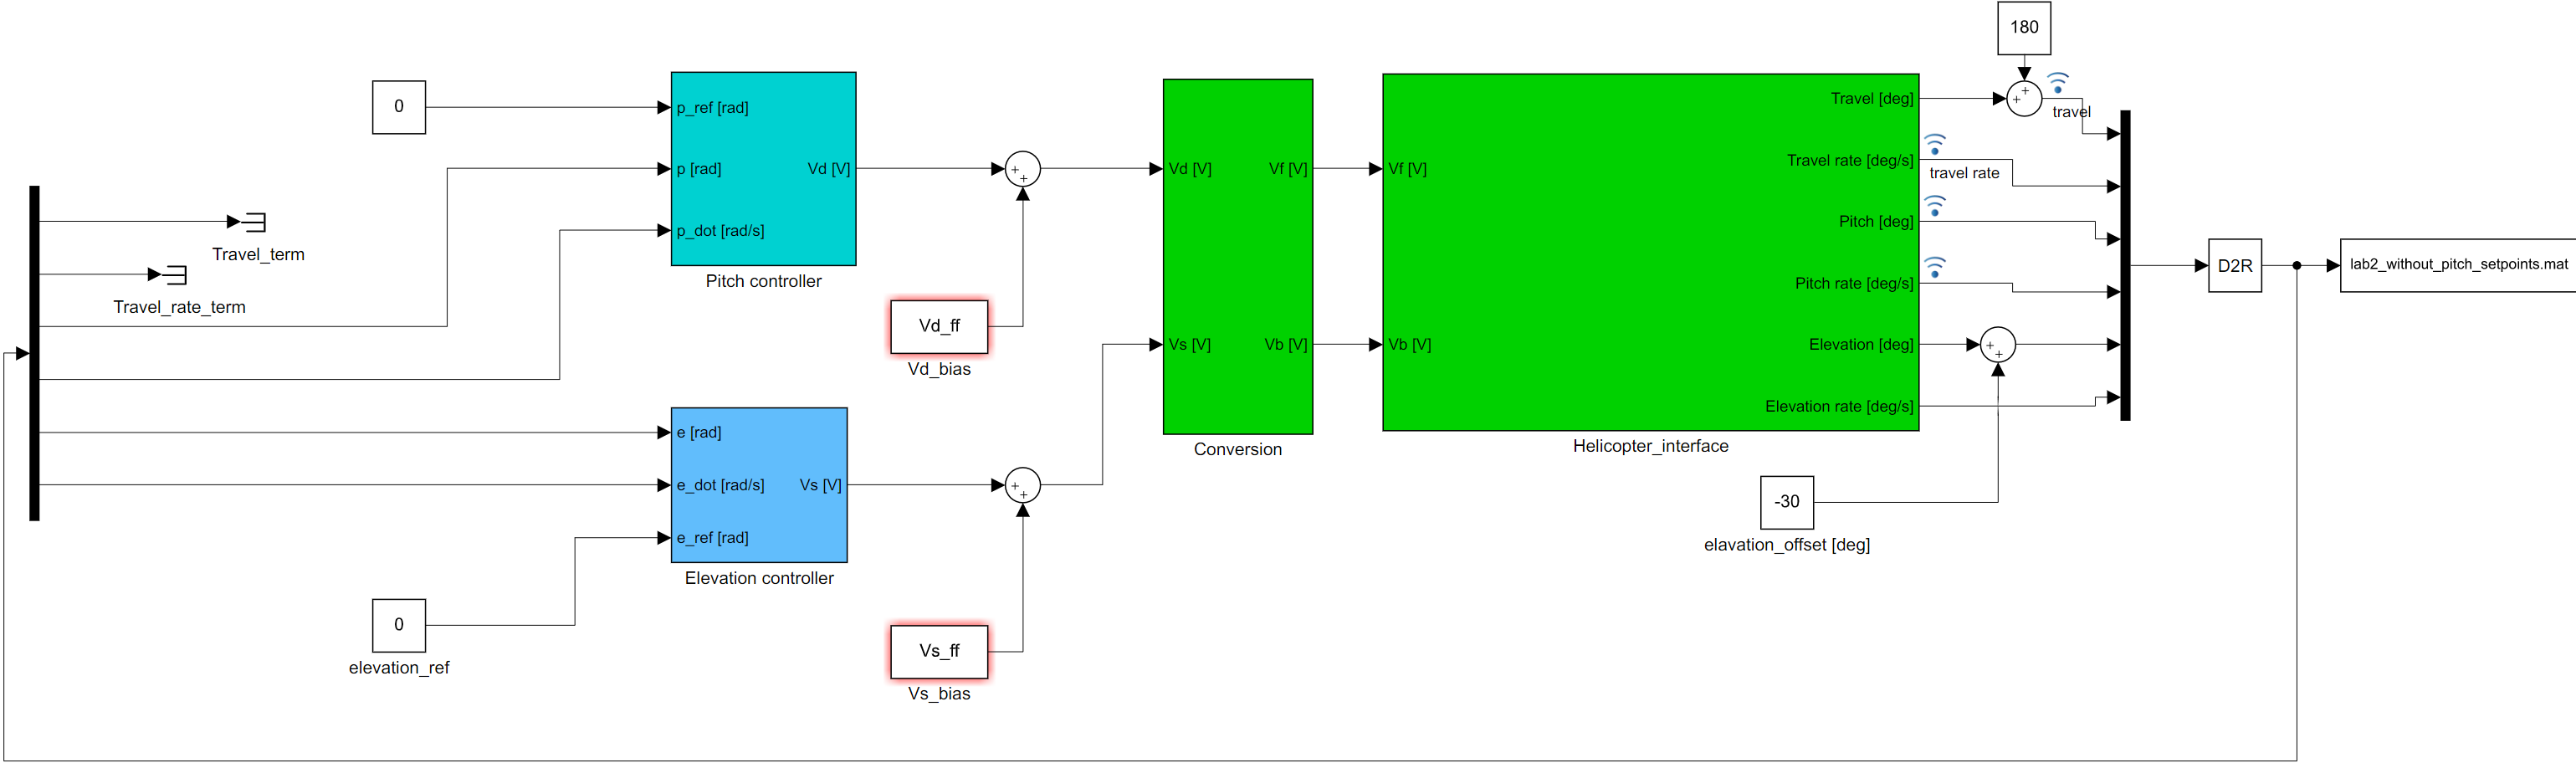
\includegraphics[width=\linewidth]{code/lab2_simulink}
	\caption{Simulink diagram used in lab 2.}
	\label{fig:lab2_simulink}
\end{figure}
\todo[inline]{Need a much better image of this.}
\end{document}